\documentclass[14pt, a4paper]{article}
\usepackage[a4paper,tmargin=2cm, bmargin=2cm, lmargin=3cm, rmargin=2.0cm]{geometry}
\usepackage{booktabs}
\usepackage{anyfontsize}
\usepackage{caption}
\usepackage{subcaption}
% \usepackage{subfigure} % deprecated and conflicts with subcaption/tocloft
% \usepackage[utf8]{inputenc} % XeLaTeX handles UTF-8 natively
\usepackage[vietnamese]{babel}
\usepackage{indentfirst}
\usepackage{color}
% \usepackage[utf8]{inputenc} % loaded above, before babel
% \usepackage{emoji} % requires LuaLaTeX; disabled for pdfLaTeX
\usepackage{amsmath}
\usepackage{amssymb}
\usepackage{amsfonts}
\usepackage{graphics}
\usepackage{graphicx}
% \usepackage{pdfpages}
\usepackage{longtable, makecell, multirow, booktabs}
% \usepackage{caption}
% \usepackage{makecell}
\usepackage{lscape}
\usepackage{pdflscape}
\usepackage{everypage}
\usepackage{titlesec}
\usepackage{tocloft} % Để tùy chỉnh mục lục
\usepackage{fontspec} % XeLaTeX/LuaLaTeX
% \usepackage[T5]{fontenc} % not needed with XeLaTeX
\usepackage[thmmarks, amsmath]{ntheorem}%
\usepackage{mdframed}
% \usepackage{xeCJK} % XeLaTeX only
\usepackage{array}
\usepackage{arydshln}
\usepackage{pgfgantt}
\usepackage[ruled,vlined,linesnumbered,resetcount,algosection]{algorithm2e}
% \usepackage{algorithm}
% \usepackage{algpseudocode}
% \usepackage{algcompatible}
% \usepackage{adjustbox} % duplicate; keep [export] variant below
\setmainfont{Arial}
% Math font separate from main (avoid Arial in equations)
\usepackage{unicode-math}
\setmathfont{texgyretermes-math.otf}
% \usepackage{newtxtext,newtxmath} % not used with Arial/XeLaTeX
% \usepackage{hyperref} % duplicate; kept once below with setup
\usepackage{tabularx}
\usepackage{float}
% \usepackage{pgfgantt} % duplicate; loaded above
% \usepackage{xcolor} % duplicate; loaded below
\usepackage{comment}
%dong khung


% ...existing code...
\usepackage{hyperref}
\hypersetup{
    colorlinks=true,           % Dùng màu chữ thay vì khung
    linkcolor=black,          % Màu link nội bộ (mục lục)
    citecolor=blue,           % Màu citation
    urlcolor=blue,            % Màu URL
    pdfborder={0 0 0},        % Tắt hoàn toàn border
}
% ...existing code...




\usepackage{framed}
\definecolor{barblue}{RGB}{153,204,254}
\definecolor{groupblue}{RGB}{51,102,254}
\definecolor{linkred}{RGB}{165,0,33}

%\renewcommand\sfdefault{phv}
%\renewcommand\mddefault{mc}

% Gây lỗi không in đậm được
% \renewcommand\bfdefault{bc}

\setganttlinklabel{s-s}{START-TO-START}
\setganttlinklabel{f-s}{FINISH-TO-START}
\setganttlinklabel{f-f}{FINISH-TO-FINISH}
\sffamily

%\input setbmp
\usepackage[export]{adjustbox}
% \usepackage{subcaption}

\usepackage{tikz}
\usepackage{pgfplots}
\pgfplotsset{compat=1.18}
%code 
\usepackage{listings}
\newcommand{\Lpagenumber}{\ifdim\textwidth=\linewidth\else\bgroup
  \dimendef\margin=0 %use \margin instead of \dimen0
  \ifodd\value{page}\margin=\oddsidemargin
  \else\margin=\evensidemargin
  \fi
  \raisebox{\dimexpr -\topmargin-\headheight-\headsep-0.5\linewidth}[0pt][0pt]{%
    \rlap{\hspace{\dimexpr \margin+\textheight+\footskip}%
    \llap{\rotatebox{90}{\thepage}}}}%
\egroup\fi}
\AddEverypageHook{\Lpagenumber}%

% Can le van ban (duplicate of geometry at top) — removed to avoid conflicts
% \usepackage[left=3cm,right=2cm,top=2cm,bottom=2cm]{geometry}
%\usepackage{fancyhdr}

% Numbering for section, subsection, etc.
\renewcommand{\thesection}{\arabic{section}}
% Section spacing and label formatting (tighter label gap)
\titlespacing{\section}{0pt}{*1.6}{0.3em}
% Show "Chương <số>. <Tiêu đề>" with moderate separation
\titleformat{\section}{\bfseries\large}{Chương\ \thesection.}{0.35em}{}
\renewcommand{\thesubsection}{\arabic{subsection}}
\titleformat{\subsection}{\bfseries\large}{\thesubsection.}{0.5em}{}

% subsubsbusection
\titleclass{\subsubsubsection}{straight}[\subsection]

\newcounter{subsubsubsection}[subsubsection]
\renewcommand\thesubsubsubsection{\thesubsubsection.\arabic{subsubsubsection}}
\renewcommand\theparagraph{\thesubsubsubsection.\arabic{paragraph}} % optional; useful if paragraphs are to be numbered

\titleformat{\subsubsubsection}
  {\normalfont\normalsize\bfseries}{\thesubsubsubsection}{1em}{}
\titlespacing*{\subsubsubsection}
{0pt}{3.25ex plus 1ex minus .2ex}{1.5ex plus .2ex}

\makeatletter
\renewcommand\paragraph{\@startsection{paragraph}{5}{\z@}%
  {3.25ex \@plus1ex \@minus.2ex}%
  {-1em}%
  {\normalfont\normalsize\bfseries}}
\renewcommand\subparagraph{\@startsection{subparagraph}{6}{\parindent}%
  {3.25ex \@plus1ex \@minus .2ex}%
  {-1em}%
  {\normalfont\normalsize\bfseries}}
\def\toclevel@subsubsubsection{4}
\def\toclevel@paragraph{5}
\def\toclevel@paragraph{6}
\def\l@subsubsubsection{\@dottedtocline{4}{7em}{4em}}
\def\l@paragraph{\@dottedtocline{5}{10em}{5em}}
\def\l@subparagraph{\@dottedtocline{6}{14em}{6em}}
\makeatother

\setcounter{secnumdepth}{4}
\setcounter{tocdepth}{4}
% ToC entries: prefix with "Chương"; ensure spacing and adequate widths
\renewcommand{\cftsecpresnum}{Chương~}
\renewcommand{\cftsecaftersnum}{.\space}
% Set section indent and number width; bring title closer in ToC
\cftsetindents{section}{0em}{7em}
\setlength{\cftsecnumwidth}{7em}


% Numbering for label itemization
\renewcommand{\baselinestretch}{1.3}
\renewcommand{\labelitemi}{$-$}
\renewcommand{\labelitemii}{$+$}

\usepackage{scrextend}
\changefontsizes{13pt}

\renewcommand{\contentsname}{MỤC LỤC}

\renewcommand{\listfigurename}{DANH SÁCH HÌNH VẼ}

\renewcommand{\listtablename}{DANH SÁCH BẢNG}

\renewcommand{\tablename}{Bảng}

\renewcommand{\figurename}{Hình}

\let\sectionautorefname\sectionautorefname
% \let\subsectionautorefname\sectionautorefname
% \let\subsubsectionautorefname\sectionautorefname
% \let\subsubsubsectionautorefname\sectionautorefname
\usepackage{textcomp}
\usepackage{listings,cleveref}
%\usepackage{minted}      % (requires -shell-escape)
\usepackage{xcolor}
\usepackage{filecontents}
\theoremheaderfont{\bfseries\upshape}
\theorembodyfont{\normalfont}
\theoremstyle{break}
\theoremseparator{\smallskip}
\newtheorem{defi}{Định nghĩa}[section]
\theoremstyle{break}
\theoremseparator{\smallskip}
\newtheorem{example}[defi]{Ví dụ}
\DeclareMathOperator*{\argmax}{argmax}
\DeclareMathOperator*{\argmin}{argmin}
\newcommand{\source}[1]{\caption*{Nguồn: {#1}} }
\newcommand{\secref}[1]{\autoref{#1}. \nameref{#1}}
\newcommand{\myparagraph}[1]{\paragraph{#1}\mbox{}\\}
\newcommand{\mysubparagraph}[1]{\subparagraph{#1}\mbox{}\\}

\newcommand\vartextvisiblespace[1][.3em]{%
  \mbox{\kern.1em\vrule height.3ex}%
  \vbox{\hrule width#1}%
  \hbox{\vrule height.3ex}
}

\newcolumntype{C}[1]{>{\centering\arraybackslash}m{#1}} 







\begin{document}
 \pagenumbering{gobble}
% \captionsetup{justification=centering}

\captionsetup[figure]{labelformat=simple, labelsep=period}

\captionsetup[table]{labelformat=simple, labelsep=period}

\begin{titlepage}
    \begin{center}
        \begin{tikzpicture}[remember picture,overlay]
        \draw[line width=3pt]
        ($(current page.north west) + (3.0cm, -2.0cm)$)
        rectangle
        ($(current page.south east) + (-2.0cm, 2.5cm)$);
        \draw[line width=0.5pt]
        ($(current page.north west) + (3.1cm, -2.1cm)$)
        rectangle
        ($(current page.south east) + (-2.1cm, 2.6cm) $);
        
        % Positioning the logo in the top left corner
        \node[anchor=north west, inner sep=1pt] at ($(current page.north west) + (3cm, -2cm)$) {
            
\includegraphics[width=155pt,height=50pt]{image/logoHutech1.png}
        };
        
        % Positioning the text in the top right corner
        \node[anchor=north east, inner sep=8pt] at ($(current page.north east) + (-2cm, -2cm)$) {
            \begin{tabular}{c}
                BỘ GIÁO DỤC VÀ ĐÀO TẠO\\
                \textbf{TRƯỜNG ĐẠI HỌC CÔNG NGHỆ TP. HCM}
            \end{tabular}
        };
        \end{tikzpicture}
        \vspace*{5cm}
        
        \textbf{\fontsize{18pt}{21pt}\selectfont ĐỒ ÁN CHUYÊN NGÀNH}\\[1.5cm]
        % \textbf{\fontsize{18pt}{21pt}\selectfont ĐỒ ÁN BẢO MẬT THÔNG TIN\\[1.5cm]
        

        \textbf{\fontsize{18pt}{15pt}\selectfont ĐỀ TÀI}
        \vspace*{0.5cm}
        

        \textbf{\fontsize{18pt}{21pt}\selectfont ỨNG DỤNG XỬ LÝ NGÔN NGỮ TỰ NHIÊN ĐỂ DỰ ĐOÁN MỨC ĐỘ HÀI LÒNG CỦA KHÁCH HÀNG QUA PHÂN TÍCH BÌNH LUẬN}\\[1.5cm] 
        \vspace*{3cm}
        
        \begin{tabular}{ll}
            %Ngành: &  \textbf{CÔNG NGHỆ THÔNG TIN}\\
            %Chuyên ngành: &  \textbf{TRÍ TUỆ NHÂN TẠO}\\[1cm]
                Giảng viên hướng dẫn: & \textbf{\fontsize{15pt}{28pt}\selectfont Trần Văn Hùng}\\
                Sinh viên thực hiện: &  \textbf{\fontsize{15pt}{21pt}\selectfont 2280602828 - Trần Tấn Tài}\\
                                 &  \textbf{\fontsize{15pt}{21pt}\selectfont 2280618597 - Trần Đình Ty}\\
                                 &  \textbf{\fontsize{15pt}{21pt}\selectfont 2280602795 - Ngô Tiến Tài}\\
                                
        \end{tabular}
        \vspace*{6cm}\\
        \textbf{\fontsize{10pt}{18pt}\selectfont TP. HỒ CHÍ MINH – THÁNG 11 NĂM 2025}
        \vfill
        
        
    \end{center}
\end{titlepage}

\newpage

\thispagestyle{empty}
%% \section*{THÔNG TIN PROJECT}
% \subsection*{Thư mục nộp bài}
% Đường dẫn: \href{https://drive.google.com/drive/folders/1JTm_curG5sIeihPt1hf0YQC0DFow91e0?usp=sharing}{\textcolor{blue}{Google Drive}}

% \subsection*{Demo}
% Đường dẫn: \href{https://youtu.be/Mjv2eUaNiik}{\textcolor{blue}{Youtube}}

% \subsection*{Cấu trúc thư mục nộp bài trên Google Drive}
% \begin{itemize}
%     \item \textbf{dataset}: Chứa tập dữ liệu sử dụng (ESD).
%     \item \textbf{source}: Mã nguồn chính của bài báo cáo.
%     \begin{itemize}
%         \item \textbf{code\_train}: Code để huấn luyện các mô hình (code cũng đã push lên \href{https://github.com/tiep271001/TriTueNhanTao_Nhom6}{\textcolor{blue}{\underline{github}}}).
%         \item \textbf{speech\_recognition\_serving}: Code triển khai mô hình (code cũng đã push lên \href{https://github.com/tiep271001/TriTueNhanTao_Nhom6}{\textcolor{blue}{\underline{github}}}).
%         \item \textbf{speech\_recognition\_app}: Code của ứng dụng (code cũng đã push lên \href{https://github.com/tiep271001/TriTueNhanTao_Nhom6}{\textcolor{blue}{\underline{github}}}).
%     \end{itemize}
%     \item \textbf{checkpoint}: Chứa checkpoint của các mô hình đã huấn luyện.
%     \item \textbf{Image\_speech\_recognition}: Chứa tất cả hình ảnh trong pptx và báo cáo.
% \end{itemize}

% \subsection*{Manual}
% Các bước để chạy web app:
% \begin{enumerate}
%     \item Truy cập \href{https://0551-2001-ee0-5006-9a10-23d3-e0c-4e83-ce7f.ngrok-free.app/}{\textcolor{blue}{đường dẫn}} đến ứng dụng 
%     \item \textbf{Click to record} để thu âm
%     \item \textbf{Click to stop recording} để kết thúc quá trình thu âm
%     \item \textbf{Send to Server} để nhận kết quả
% \end{enumerate}

% Đường link cập nhật của ứng dụng tại \href{https://drive.google.com/drive/folders/1JTm_curG5sIeihPt1hf0YQC0DFow91e0?usp=sharing}{\textcolor{blue}{Google Drive}}
% \newpage
\tableofcontents
\thispagestyle{empty}
\newpage
\thispagestyle{empty}
% \listoftables
% \newpage
\listoffigures
\newpage
% \setcounter{secnumdepth}{0} % Tắt đánh số section
\listoftables
\clearpage

\setcounter{secnumdepth}{9} % Đảm bảo đánh số cho các cấp thấp hơn

\pagenumbering{arabic}
% \section*{THÔNG TIN PROJECT}
% \subsection*{Thư mục nộp bài}
% Đường dẫn: \href{https://drive.google.com/drive/folders/1JTm_curG5sIeihPt1hf0YQC0DFow91e0?usp=sharing}{\textcolor{blue}{Google Drive}}

% \subsection*{Demo}
% Đường dẫn: \href{https://youtu.be/Mjv2eUaNiik}{\textcolor{blue}{Youtube}}

% \subsection*{Cấu trúc thư mục nộp bài trên Google Drive}
% \begin{itemize}
%     \item \textbf{dataset}: Chứa tập dữ liệu sử dụng (ESD).
%     \item \textbf{source}: Mã nguồn chính của bài báo cáo.
%     \begin{itemize}
%         \item \textbf{code\_train}: Code để huấn luyện các mô hình (code cũng đã push lên \href{https://github.com/tiep271001/TriTueNhanTao_Nhom6}{\textcolor{blue}{\underline{github}}}).
%         \item \textbf{speech\_recognition\_serving}: Code triển khai mô hình (code cũng đã push lên \href{https://github.com/tiep271001/TriTueNhanTao_Nhom6}{\textcolor{blue}{\underline{github}}}).
%         \item \textbf{speech\_recognition\_app}: Code của ứng dụng (code cũng đã push lên \href{https://github.com/tiep271001/TriTueNhanTao_Nhom6}{\textcolor{blue}{\underline{github}}}).
%     \end{itemize}
%     \item \textbf{checkpoint}: Chứa checkpoint của các mô hình đã huấn luyện.
%     \item \textbf{Image\_speech\_recognition}: Chứa tất cả hình ảnh trong pptx và báo cáo.
% \end{itemize}

% \subsection*{Manual}
% Các bước để chạy web app:
% \begin{enumerate}
%     \item Truy cập \href{https://0551-2001-ee0-5006-9a10-23d3-e0c-4e83-ce7f.ngrok-free.app/}{\textcolor{blue}{đường dẫn}} đến ứng dụng 
%     \item \textbf{Click to record} để thu âm
%     \item \textbf{Click to stop recording} để kết thúc quá trình thu âm
%     \item \textbf{Send to Server} để nhận kết quả
% \end{enumerate}

% Đường link cập nhật của ứng dụng tại \href{https://drive.google.com/drive/folders/1JTm_curG5sIeihPt1hf0YQC0DFow91e0?usp=sharing}{\textcolor{blue}{Google Drive}}
% \newpage

\newpage



\section{\textbf{LỜI MỞ ĐẦU}}
Trong thời đại thương mại điện tử phát triển mạnh mẽ, việc đánh giá và phân tích cảm xúc (sentiment analysis) của khách hàng đối với sản phẩm đã trở thành yếu tố quan trọng giúp doanh nghiệp cải thiện chất lượng dịch vụ và người dùng đưa ra quyết định mua hàng sáng suốt. Các nền tảng thương mại điện tử hiện đại không chỉ cung cấp không gian mua sắm mà còn cần tích hợp trí tuệ nhân tạo (artificial intelligence) để phân tích phản hồi của khách hàng một cách tự động và chính xác.

Hệ thống đánh giá sản phẩm với AI ra đời nhằm giải quyết bài toán phân tích cảm xúc từ bình luận và đánh giá của khách hàng, sử dụng công nghệ xử lý ngôn ngữ tự nhiên (natural language processing) tiên tiến. Với khả năng phân tích tự động các bình luận thành các mức độ hài lòng (tích cực/positive, tiêu cực/negative, trung tính/neutral), hệ thống giúp doanh nghiệp thấu hiểu nhanh chóng phản hồi của khách hàng, từ đó cải thiện chất lượng sản phẩm và dịch vụ.

Chính vì vậy, nhóm quyết định thực hiện đồ án “Xây dựng hệ thống đánh giá sản phẩm với AI” với mục tiêu phát triển một hệ thống hoàn chỉnh bao gồm Web App và Mobile App, tích hợp mô hình AI sử dụng PhoBERT để phân tích cảm xúc tiếng Việt, cho phép người dùng xem sản phẩm, đánh giá và nhận được phân tích tự động về mức độ hài lòng của cộng đồng.

\newpage

\section{\textbf{LỜI CAM ĐOAN}}

Nhóm xin cam đoan rằng đồ án \textbf{“Ứng dụng xử lý ngôn ngữ tự nhiên để dự đoán mức độ hài lòng của khách hàng qua phân tích bình luận”} là kết quả nghiên cứu độc lập và làm việc miệt mài của tất cả thành viên trong nhóm, dưới sự hướng dẫn của giảng viên \textbf{Trần Văn Hùng}.

Toàn bộ nội dung trong đồ án này được nhóm tự mày mò nghiên cứu, phân tích và triển khai dựa trên kiến thức đã học tập, kinh nghiệm thực tế và các tài liệu tham khảo có trích dẫn nguồn gốc rõ ràng. Nhóm cam kết đây là sản phẩm trí tuệ hoàn toàn độc lập, không sao chép hoặc sử dụng trái phép nội dung từ bất kỳ nguồn nào mà không ghi rõ nguồn gốc.

Nếu phát hiện có bất kỳ hành vi đạo văn hoặc gian lận nào trong đồ án này, nhóm xin chịu hoàn toàn trách nhiệm trước nhà trường và hội đồng đánh giá.

Nhóm xin chân thành cảm ơn!

 

\newpage

\section{\textbf{TỔNG QUAN VỀ VERITASHOP}}

\subsection{Giới thiệu}
Trong bối cảnh TMĐT bùng nổ, nhu cầu tự động phân tích cảm xúc và dự đoán mức độ hài lòng từ bình luận sản phẩm ngày càng cấp thiết. VeritaShop tập trung phát triển mô hình NLP (PhoBERT) để phân loại cảm xúc tiếng Việt chính xác và tích hợp vào nền tảng TMĐT kiến trúc microservices, nhằm nâng cao trải nghiệm người dùng và hỗ trợ quyết định dựa trên dữ liệu.

\subsection{Tổng quan hệ thống}
\subsubsection{Mục đích hệ thống}
VeritaShop là nền tảng TMĐT thông minh: hiển thị sản phẩm, thu nhận đánh giá và cung cấp phân tích cảm xúc tự động. Mục tiêu chính:
\begin{itemize}
    \item Nền tảng giao diện thân thiện, responsive, hỗ trợ sáng/tối.
    \item Tích hợp PhoBERT phân tích cảm xúc bình luận.
    \item Dự đoán mức độ hài lòng (tích cực/trung tính/tiêu cực) tự động.
    \item Tối ưu hiệu năng với microservices, containerization và cloud.
\end{itemize}
VeritaShop không cạnh tranh trực tiếp với các nền tảng lớn, mà cung cấp giải pháp quy mô vừa, ứng dụng AI để cải thiện phân tích cảm xúc, dự đoán xu hướng và trải nghiệm người dùng.

\subsubsection{Khảo sát các sản phẩm tương tự}
Các nền tảng như Shopee, Lazada, Tiki còn hạn chế về phân tích cảm xúc và dự đoán hài lòng:
\begin{itemize}
    \item \textbf{Shopee}: Đánh giá cơ bản, thiếu phân tích cảm xúc tự động và dự đoán xu hướng.
    \item \textbf{Lazada}: Giao diện tốt, chưa tích hợp AI phân tích cảm xúc chính xác.
    \item \textbf{Tiki}: Hỗ trợ media, còn yếu ở phân tích ngữ nghĩa/ngữ cảnh bình luận.
\end{itemize}
Hệ thống đề xuất cải tiến:
\begin{itemize}
    \item Tích hợp PhoBERT phân tích cảm xúc tiếng Việt.
    \item Dự đoán mức độ hài lòng tự động, chính xác.
    \item Trực quan hóa kết quả để hỗ trợ quyết định.
\end{itemize}

\subsubsection{Yêu cầu hoạt động của ứng dụng}
\subsubsubsection{Phần dành cho người dùng cuối}
Chức năng chính:
\begin{itemize}
    \item \textbf{Đăng ký/đăng nhập}: Xác thực email, JWT.
    \item \textbf{Hồ sơ}: Cập nhật thông tin, ảnh đại diện.
    \item \textbf{Duyệt/tìm kiếm}: Danh sách, bộ lọc, chi tiết sản phẩm.
    \item \textbf{Đánh giá/bình luận}: Viết đánh giá, xem phân tích cảm xúc cộng đồng.
    \item \textbf{Mua hàng}: Giỏ hàng, thanh toán, theo dõi đơn.
    \item \textbf{Hỗ trợ AI}: Chatbot gợi ý và trợ giúp.
\end{itemize}

\subsubsubsection{Phần dành cho người bán/doanh nghiệp}
\begin{itemize}
    \item \textbf{Sản phẩm}: CRUD danh mục/sản phẩm.
    \item \textbf{Thống kê}: Doanh số, đánh giá, mức độ hài lòng.
    \item \textbf{Phân tích cảm xúc}: Báo cáo chi tiết theo sản phẩm.
    \item \textbf{Đơn hàng}: Xử lý và theo dõi trạng thái.
    \item \textbf{Tương tác khách hàng}: Phản hồi bình luận/đánh giá.
\end{itemize}

\subsubsubsection{Phần dành cho quản trị viên}
\begin{itemize}
    \item \textbf{Người dùng}: Quản lý và khóa tài khoản.
    \item \textbf{Sản phẩm}: Duyệt và kiểm soát chất lượng.
    \item \textbf{Monitoring}: Theo dõi hiệu suất và sự cố.
    \item \textbf{Dashboard}: Quản trị tổng quan.
\end{itemize}

\subsection{Thiết kế tương tác}
Giao diện thân thiện, responsive, hỗ trợ sáng/tối trên desktop/mobile. Thành phần chính:
\begin{itemize}
    \item \textbf{Trang chủ}: Sản phẩm nổi bật/khuyến mãi, chỉ số hài lòng, lazy loading.
    \item \textbf{Trang sản phẩm}: Chi tiết, đánh giá và phân tích cảm xúc.
    \item \textbf{Giỏ hàng/Thanh toán}: Thao tác đơn giản, an toàn.
    \item \textbf{Hồ sơ}: Thông tin cá nhân, lịch sử mua, đánh giá.
    \item \textbf{Bảng điều khiển người bán}: Quản lý sản phẩm, đơn và thống kê.
    \item \textbf{Admin dashboard}: Quản lý hệ thống, người dùng, sản phẩm.
    \item \textbf{Chatbot AI}: Tìm kiếm, giải đáp, gợi ý.
\end{itemize}

\subsection{Phương pháp tiếp cận và giải quyết vấn đề}
\subsubsection{Mô hình tổng quát hệ thống}
Kiến trúc Microservices kết hợp công nghệ NLP và hạ tầng hiện đại:
\begin{itemize}
    \item \textbf{Frontend}: Next.js (Web), Flutter (Mobile) responsive, hiệu năng cao.
    \item \textbf{Microservices Backend}: Node.js (NestJS/TypeScript) cho nghiệp vụ; Python (FastAPI) cho AI.
    \item \textbf{AI Service}: PhoBERT phân tích cảm xúc bình luận.
    \item \textbf{Cơ sở dữ liệu}: PostgreSQL (cấu trúc), MongoDB (phân tích/logs).
    \item \textbf{DevOps}: Docker, Kubernetes, GitHub Actions, AWS.
\end{itemize}

\subsubsection{Phương pháp xây dựng phần mềm}
Áp dụng Agile trên kiến trúc Microservices, gồm:
\begin{itemize}
    \item Phân tích yêu cầu.
    \item Thiết kế kiến trúc (Microservices, Layered), CSDL và mô hình AI.
    \item Phát triển services (User/Auth, Product, Payment, AI) với Prisma ORM/PhoBERT.
    \item Tích hợp/kiểm thử; áp dụng Saga cho giao dịch phân tán.
    \item DevOps: Docker, Kubernetes, GitHub Actions CI/CD.
\end{itemize}

\subsubsection{Kiến trúc phần mềm}
Kiến trúc Microservices áp dụng Layered Architecture cho từng service:

Presentation Layer (Controllers):
- Xử lý HTTP, validation/authentication, logging

Business Logic Layer (Services):
- Logic nghiệp vụ, xử lý use cases, quản lý giao dịch

Data Access Layer (Repositories):
- Truy cập database, CRUD, tối ưu truy vấn, caching

\begin{itemize}
    \item \textbf{Frontend}: Next.js với App Router và Server Components cho Web App, Flutter với BLoC pattern cho Mobile App.
    \item \textbf{Microservices Backend}:
    \begin{itemize}
        \item Node.js với Express.js và TypeScript cho User/Auth, Product, Payment services được tổ chức theo Layered Architecture (Controllers → Services → Repositories)
        \item Python với FastAPI cho AI service phân tích cảm xúc với kiến trúc phân lớp rõ ràng
        \item Prisma ORM để truy cập cơ sở dữ liệu type-safe
    \end{itemize}
    \item \textbf{Cơ sở dữ liệu}: PostgreSQL cho dữ liệu có cấu trúc, MongoDB cho dữ liệu phân tích và logs.
    \item \textbf{Giao tiếp}: REST API và MQ (RabbitMQ/Kafka) giữa các service.
\end{itemize}

\subsubsection{Công nghệ triển khai hệ thống}
\subsubsubsection{Microservices Backend}
\begin{itemize}
    \item \textbf{Node.js (Express.js + TypeScript)}: Tổ chức theo Layered Architecture (Controllers/Services/Repositories) với middleware linh hoạt.
    \item \textbf{Python (FastAPI)}: Dịch vụ AI async hiệu năng cao, tự động hoá OpenAPI.
    \item \textbf{Prisma ORM}: Truy cập CSDL type-safe, hỗ trợ migrations và query builder.
    \item \textbf{PostgreSQL}: CSDL quan hệ cho dữ liệu nghiệp vụ (users, products, orders).
    \item \textbf{MongoDB}: NoSQL cho phân tích, logs và cache.
    \item \textbf{RabbitMQ/Kafka}: Hàng đợi thông điệp cho giao tiếp bất đồng bộ giữa services.
\end{itemize}

\subsubsubsection{Frontend}
\begin{itemize}
    \item \textbf{Next.js}: SSR/SSG với App Router và Server Components để tối ưu hiệu năng.
    \item \textbf{Flutter}: Ứng dụng di động đa nền tảng (iOS/Android) bằng Dart.
    \item \textbf{Redux Toolkit}: Quản lý state cho React.
    \item \textbf{Material-UI/Ant Design}: Thư viện UI thống nhất giao diện.
\end{itemize}

\subsubsubsection{AI/ML}
\begin{itemize}
    \item \textbf{PhoBERT}: Mô hình tiếng Việt SOTA cho phân tích cảm xúc.
    \item \textbf{Transformers (Hugging Face)}: Hạ tầng mô hình hoá và suy luận NLP.
    \item \textbf{TensorFlow/PyTorch}: Huấn luyện và triển khai mô hình học sâu.
    \item \textbf{Scikit-learn}: Tiền xử lý và đánh giá mô hình.
\end{itemize}

\subsubsubsection{DevOps \& Infrastructure}
\begin{itemize}
    \item \textbf{Docker}: Đóng gói ứng dụng và dependencies dưới dạng container.
    \item \textbf{Kubernetes}: Orchestrate và quản lý containers ở môi trường production.
    \item \textbf{GitHub Actions}: CI/CD tự động cho test/build/deploy.
    \item \textbf{AWS}: Hạ tầng cloud (EKS, RDS, S3, ECR, ...).
    \item \textbf{Prometheus \& Grafana}: Giám sát và cảnh báo.
    \item \textbf{ELK Stack}: Ghi log tập trung (Elasticsearch, Logstash, Kibana).
\end{itemize}

% \subsection{Tổng kết chương}
% Chương này đã trình bày tổng quan về VeritaShop - hệ thống phân tích cảm xúc sản phẩm sử dụng AI tiên tiến. Nội dung bao gồm giới thiệu dự án, khảo sát thị trường, yêu cầu chức năng, thiết kế giao diện và phương pháp triển khai. Hệ thống áp dụng kiến trúc microservices với mô hình phân lớp, sử dụng các công nghệ hiện đại để phân tích bình luận và dự đoán mức độ hài lòng khách hàng. Chương tiếp theo sẽ trình bày cơ sở lý thuyết về xử lý ngôn ngữ tự nhiên và mô hình học máy.

\newpage
%
% Section IV content provided by user
%
\section{CƠ SỞ LÝ THUYẾT}\label{sec:theory_support}
\subsection{Giới thiệu bài toán}

Trong bối cảnh bùng nổ thương mại điện tử tại Việt Nam, việc phân tích và hiểu rõ cảm xúc của khách hàng từ bình luận sản phẩm đã trở thành yếu tố then chốt giúp doanh nghiệp cải thiện chất lượng dịch vụ và tối ưu hóa sản phẩm. Tuy nhiên, ngôn ngữ bình luận tiếng Việt thường chứa nhiều yếu tố phi chuẩn như tiếng lóng, viết tắt, biểu tượng cảm xúc và cấu trúc câu ngắn gọn, tạo ra thách thức lớn cho các hệ thống phân tích cảm xúc truyền thống.

Nghiên cứu này tập trung phát triển hệ thống VeritaShop tích hợp mô hình PhoBERT - một mô hình ngôn ngữ tiên tiến được thiết kế riêng cho tiếng Việt - nhằm giải quyết bài toán phân tích cảm xúc đa chiều từ bình luận sản phẩm. Mục tiêu chính là xây dựng một hệ thống có khả năng tự động phân loại chính xác cảm xúc khách hàng (tích cực, tiêu cực, trung tính) và cung cấp dự đoán đáng tin cậy về mức độ hài lòng, từ đó hỗ trợ doanh nghiệp trong việc ra quyết định chiến lược dựa trên dữ liệu thực tế.

Việc giải quyết bài toán này mang ý nghĩa thực tiễn quan trọng, không chỉ giúp doanh nghiệp nắm bắt nhanh chóng phản hồi thị trường mà còn nâng cao trải nghiệm người dùng thông qua việc cung cấp thông tin phân tích đáng tin cậy. Hệ thống được thiết kế với kiến trúc microservices linh hoạt, cho phép triển khai hiệu quả trong môi trường sản xuất và đáp ứng yêu cầu phân tích thời gian thực, góp phần thúc đẩy chuyển đổi số trong lĩnh vực thương mại điện tử tại Việt Nam.
\subsection{Các nghiên cứu liên quan}

Các hướng tiếp cận phân tích cảm xúc đã tiến hóa từ mô hình dựa trên đặc trưng thủ công sang học biểu diễn sâu quy mô lớn. Giai đoạn đầu, các đặc trưng thống kê (bag-of-words/TF–IDF) kết hợp SVM/Naive Bayes giúp triển khai nhanh nhưng kém khả năng nắm bắt ngữ nghĩa và phụ thuộc mạnh vào tiền xử lý, đặc biệt với bình luận tiếng Việt giàu tiếng lóng/emoji. Với học sâu, CNN chứng minh hiệu quả trên văn bản ngắn bằng các bộ lọc trượt \\cite{kim-2014-convolutional}, LSTM khắc phục phụ thuộc dài hạn \\cite{10.1162/neco.1997.9.8.1735}, và Transformer cùng cơ chế tự chú ý mở ra bước nhảy vọt về mô hình hóa quan hệ toàn cục \\cite{vaswani2017attention}, đặt nền cho làn sóng mô hình tiền huấn luyện.

Trong bối cảnh tiếng Việt, mô hình đa ngôn ngữ (mBERT) cho kết quả ban đầu nhưng chưa đặc tả tốt hiện tượng ngôn ngữ bản địa; các mô hình chuyên biệt như PhoBERT \\cite{phobert} cho thấy ưu thế rõ rệt trên tác vụ phân loại và cảm xúc nhờ tiền huấn luyện trên kho ngữ liệu lớn tiếng Việt. Dù vậy, phần lớn công trình vẫn bộc lộ các hạn chế: (i) miền thương mại điện tử với bình luận ngắn, nhiễu, lệch nhãn ít được xử lý có hệ thống; (ii) mất cân bằng dữ liệu thường bị xem nhẹ, ảnh hưởng trực tiếp tới F1 của lớp thiểu số; (iii) ít nghiên cứu bàn tới tích hợp thời gian thực ở mức hệ thống, bao gồm độ trễ suy luận, khả năng mở rộng và giám sát vận hành.

Nghiên cứu này định vị đóng góp bằng cách tổng hợp các tiến bộ trên theo hướng thực dụng: tinh chỉnh PhoBERT cho miền TMĐT tiếng Việt, kết hợp chiến lược học chống lệch (ví dụ focal loss) để cải thiện độ bền với mất cân bằng, và triển khai trong kiến trúc microservices hướng suy luận thời gian thực. Cách tiếp cận này vừa kế thừa sức mạnh biểu diễn của mô hình tiền huấn luyện, vừa khắc phục các khoảng trống về dữ liệu và triển khai mà nhiều nghiên cứu trước chưa giải quyết triệt để.

\subsection{Mô hình PhoBERT}
% \subsubsection{Quy trình tinh chỉnh}
% \subsubsection{Xử lý dữ liệu và hàm mất mát}
% \subsubsection{Tích hợp vào hệ thống}
\begin{comment}
Phần này trình bày nền tảng khoa học cho bài toán phân tích cảm xúc đối với bình luận sản phẩm tiếng Việt, gồm đặc tả nhiệm vụ, tổng quan các phương pháp nghiên cứu và cơ chế hoạt động của mô hình PhoBERT mà dự án lựa chọn.


Phân tích cảm xúc (Sentiment Analysis) tìm cách suy luận thái độ của người viết thông qua văn bản. Trong ngữ cảnh thương mại điện tử, tác vụ thường được rút gọn thành phân loại cảm xúc của bình luận vào các nhãn rời rạc. Đồ án VeritaShop tập trung vào tập bình luận tiếng Việt có độ dài ngắn, nhiều ký tự biểu cảm, tiếng lóng và viết tắt, đồng thời gán mỗi mẫu vào ba nhãn \textit{tích cực}, \textit{trung tính} hoặc \textit{tiêu cực}. Bài toán đặt ra ba thách thức chính: (i) dữ liệu mất cân bằng, tỷ lệ bình luận tích cực vượt trội khiến mô hình dễ thiên lệch, (ii) ngôn ngữ phi chuẩn làm suy giảm khả năng hiểu ngữ nghĩa, và (iii) yêu cầu suy luận thời gian thực để tích hợp vào quy trình phục vụ khách hàng. Do đó hệ thống cần quy trình tiền xử lý chuẩn hóa, biểu diễn ngôn ngữ mạnh và chiến lược tối ưu hóa phù hợp để duy trì độ chính xác ổn định.

\subsection{Các nghiên cứu liên quan}
Các hướng tiếp cận truyền thống sử dụng đặc trưng thống kê như bag-of-words, TF-IDF kết hợp với SVM hoặc Naive Bayes giúp triển khai nhanh nhưng thiếu khả năng nắm bắt ngữ nghĩa và phụ thuộc mạnh vào tiền xử lý thủ công. Sự phát triển của học sâu đã mở ra các mô hình biểu diễn ngữ nghĩa hiệu quả hơn:
\begin{itemize}
    \item Kim \cite{kim-2014-convolutional} chứng minh CNN với bộ lọc trượt có khả năng khai thác cụm từ quan trọng khi phân loại văn bản ngắn.
    \item LSTM \cite{10.1162/neco.1997.9.8.1735} giải quyết vấn đề phụ thuộc dài hạn trong câu, phù hợp với dữ liệu hội thoại và đánh giá.
    \item Kiến trúc Transformer cùng cơ chế Attention \cite{vaswani2017attention} cho phép mô hình hóa quan hệ toàn cục giữa các token, là tiền đề cho các mô hình ngôn ngữ pre-training.
    \item Các mô hình pre-training dành cho tiếng Việt như PhoBERT \cite{phobert}, viBERT hay viBART chứng minh hiệu quả vượt trội so với mBERT đa ngôn ngữ trong các tác vụ phân loại và phân tích cảm xúc tiếng Việt.
\end{itemize}
Những công trình trên cho thấy xu hướng chuyển dịch từ việc tự thiết kế đặc trưng sang tận dụng biểu diễn ngữ nghĩa học được từ dữ liệu lớn. Dựa trên các kết quả đó, dự án lựa chọn PhoBERT làm nền tảng và tinh chỉnh thêm để thích ứng với miền dữ liệu thương mại điện tử.


PhoBERT được xây dựng dựa trên BERT nước đôi với 12 lớp encoder, 12 đầu chú ý và chiều ẩn 768, được tiền huấn luyện trên hơn 20GB văn bản tiếng Việt chuẩn hóa theo Byte-Pair Encoding \cite{phobert}. Khối encoder học biểu diễn ngữ cảnh hai chiều, nhờ đó vector [CLS] cuối cùng mang thông tin toàn câu phục vụ phân loại.


Trong giai đoạn fine-tuning cho VeritaShop, token [CLS] được đưa qua một lớp dense ba nhãn, áp dụng Dropout 0.1 để giảm quá khớp và tối ưu bằng AdamW với lịch điều chỉnh learning rate dạng cosine. Chiến lược này cho phép mô hình hội tụ ổn định trên bộ dữ liệu không lớn.


Bộ dữ liệu bình luận bị lệch nhãn về phía tích cực, vì vậy nhóm áp dụng chiến lược tăng cường và cân bằng gồm: chuẩn hóa Unicode, chuẩn hóa viết tắt, loại bỏ ký tự nhiễu, giữ lại emoji quan trọng và sử dụng tokenizer BPE của PhoBERT với chiều dài tối đa 256 token. Focal loss với $\gamma = 2$ và hệ số $\alpha$ theo từng lớp được lựa chọn thay cho cross-entropy chuẩn để tập trung hơn vào các mẫu khó, cải thiện F1-score lớp tiêu cực.

\subsubsection{Tích hợp vào hệ thống}
PhoBERT được đóng gói thành AI Service (FastAPI) và giao tiếp với các microservice khác thông qua REST nội bộ. Product Service và Review Service xây dựng bằng Node.js kết hợp Prisma/PostgreSQL chịu trách nhiệm lưu trữ dữ liệu, trong khi Notification Service cảnh báo xu hướng tiêu cực. Toàn bộ cụm dịch vụ được container hóa bằng Docker, theo dõi bằng Prometheus/Grafana và có thể mở rộng ngang khi lưu lượng bình luận tăng.

Nhờ đặc trưng ngôn ngữ giàu ngữ cảnh và quy trình tinh chỉnh phù hợp, PhoBERT đáp ứng tốt yêu cầu phân tích cảm xúc thời gian thực của hệ thống VeritaShop.
\end{comment}

\newpage

\section{\textbf{THIẾT KẾ HỆ THỐNG}}
% \newpage
% \section{\textbf{CHƯƠNG 3: Phân tích thiết kế hệ thống}}

% \subsection{Phân Tích Hệ Thống}

% \subsubsection{Biểu đồ Usecase}


% \textbf{Use Case Tổng quát} \\
% \begin{figure}[H]
%     \centering
%     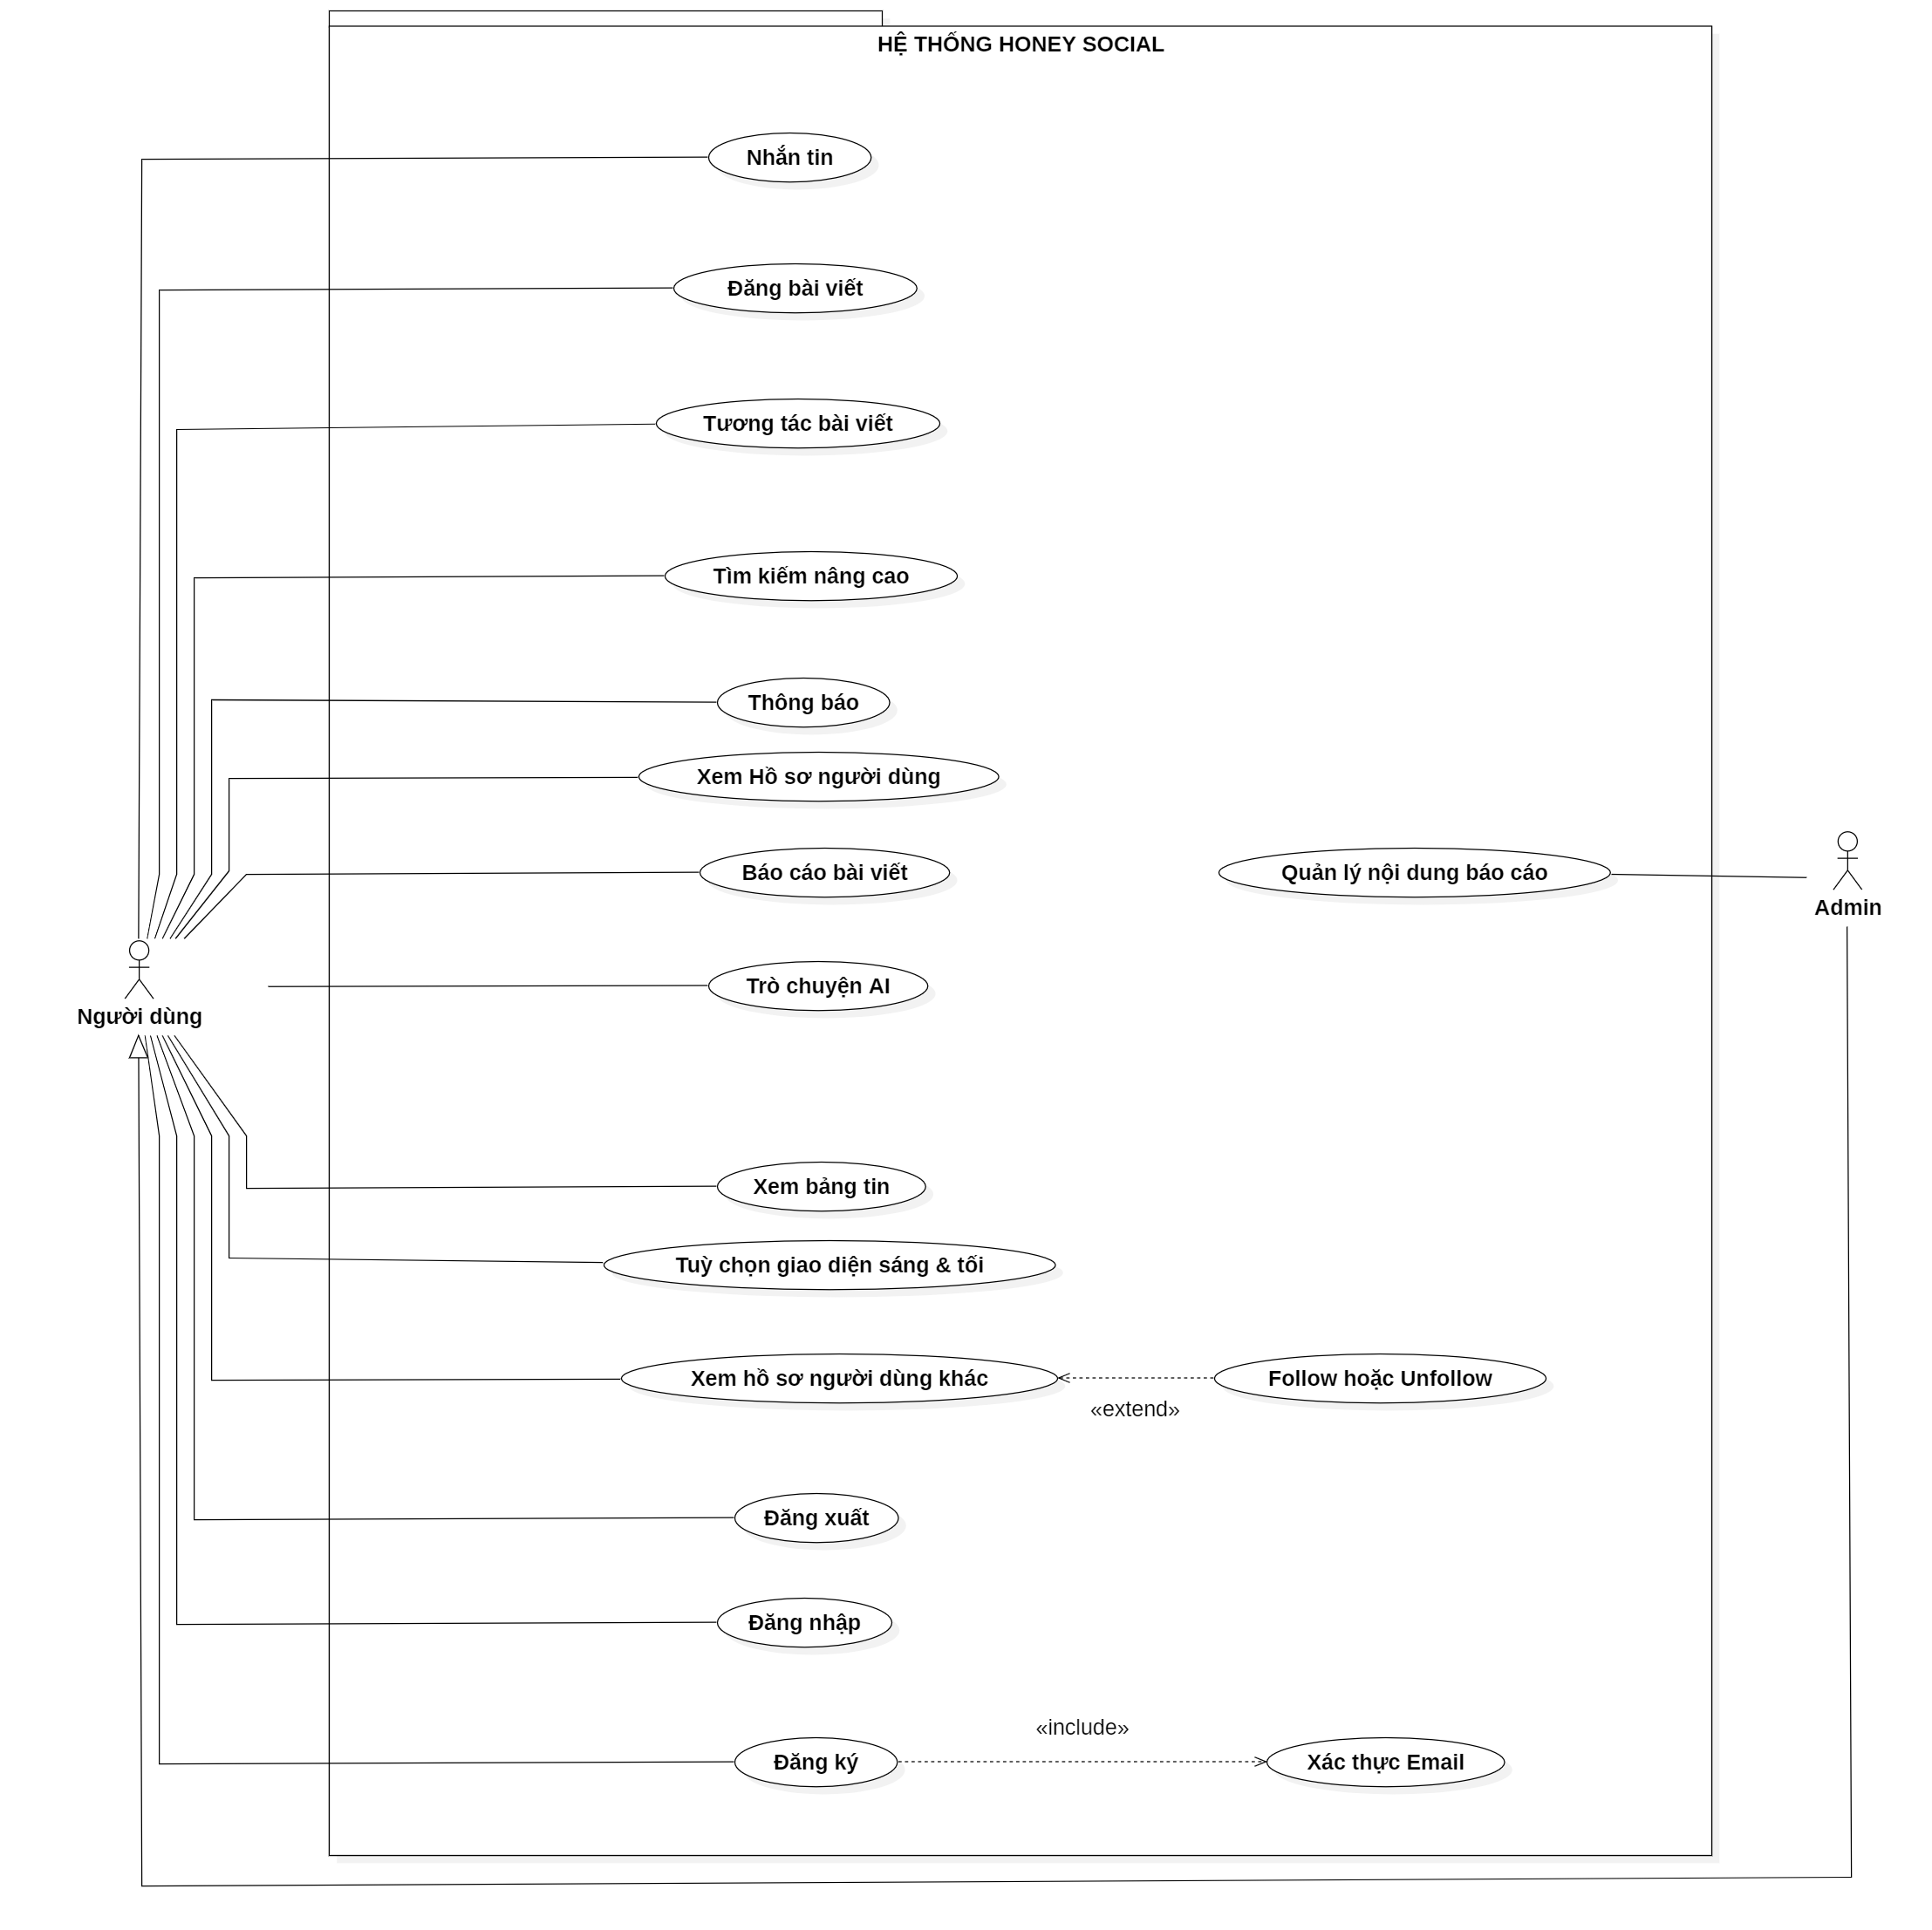
\includegraphics[width=1\textwidth]{image/MoHinh/1.png}
%     \caption{Hình ảnh Use Case Tổng quát}
%     \label{fig:use_case_tong_quat}
% \end{figure}
% Các chức năng được bao bởi hệ thống \textbf{HỆ THỐNG HONEY SOCIAL} và là những hành động mà người dùng có thể thực hiện như sau:

% \begin{itemize}
%     \item Nhắn tin
%     \item Đăng bài viết
%     \item Tương tác bài viết: Thích, bình luận, chia sẻ,...
%     \item Tìm kiếm nâng cao
%     \item Thông báo
%     \item Xem hồ sơ người dùng
%     \item Báo cáo bài viết
%     \item Trò chuyện AI
%     \item Xem bảng tin
%     \item Tùy chọn giao diện sáng \& tối
%     \item Đăng nhập
%     \item Đăng xuất
% \end{itemize}

% \textbf{Đăng bài viết} \\
% \begin{figure}[H]
%     \centering
%     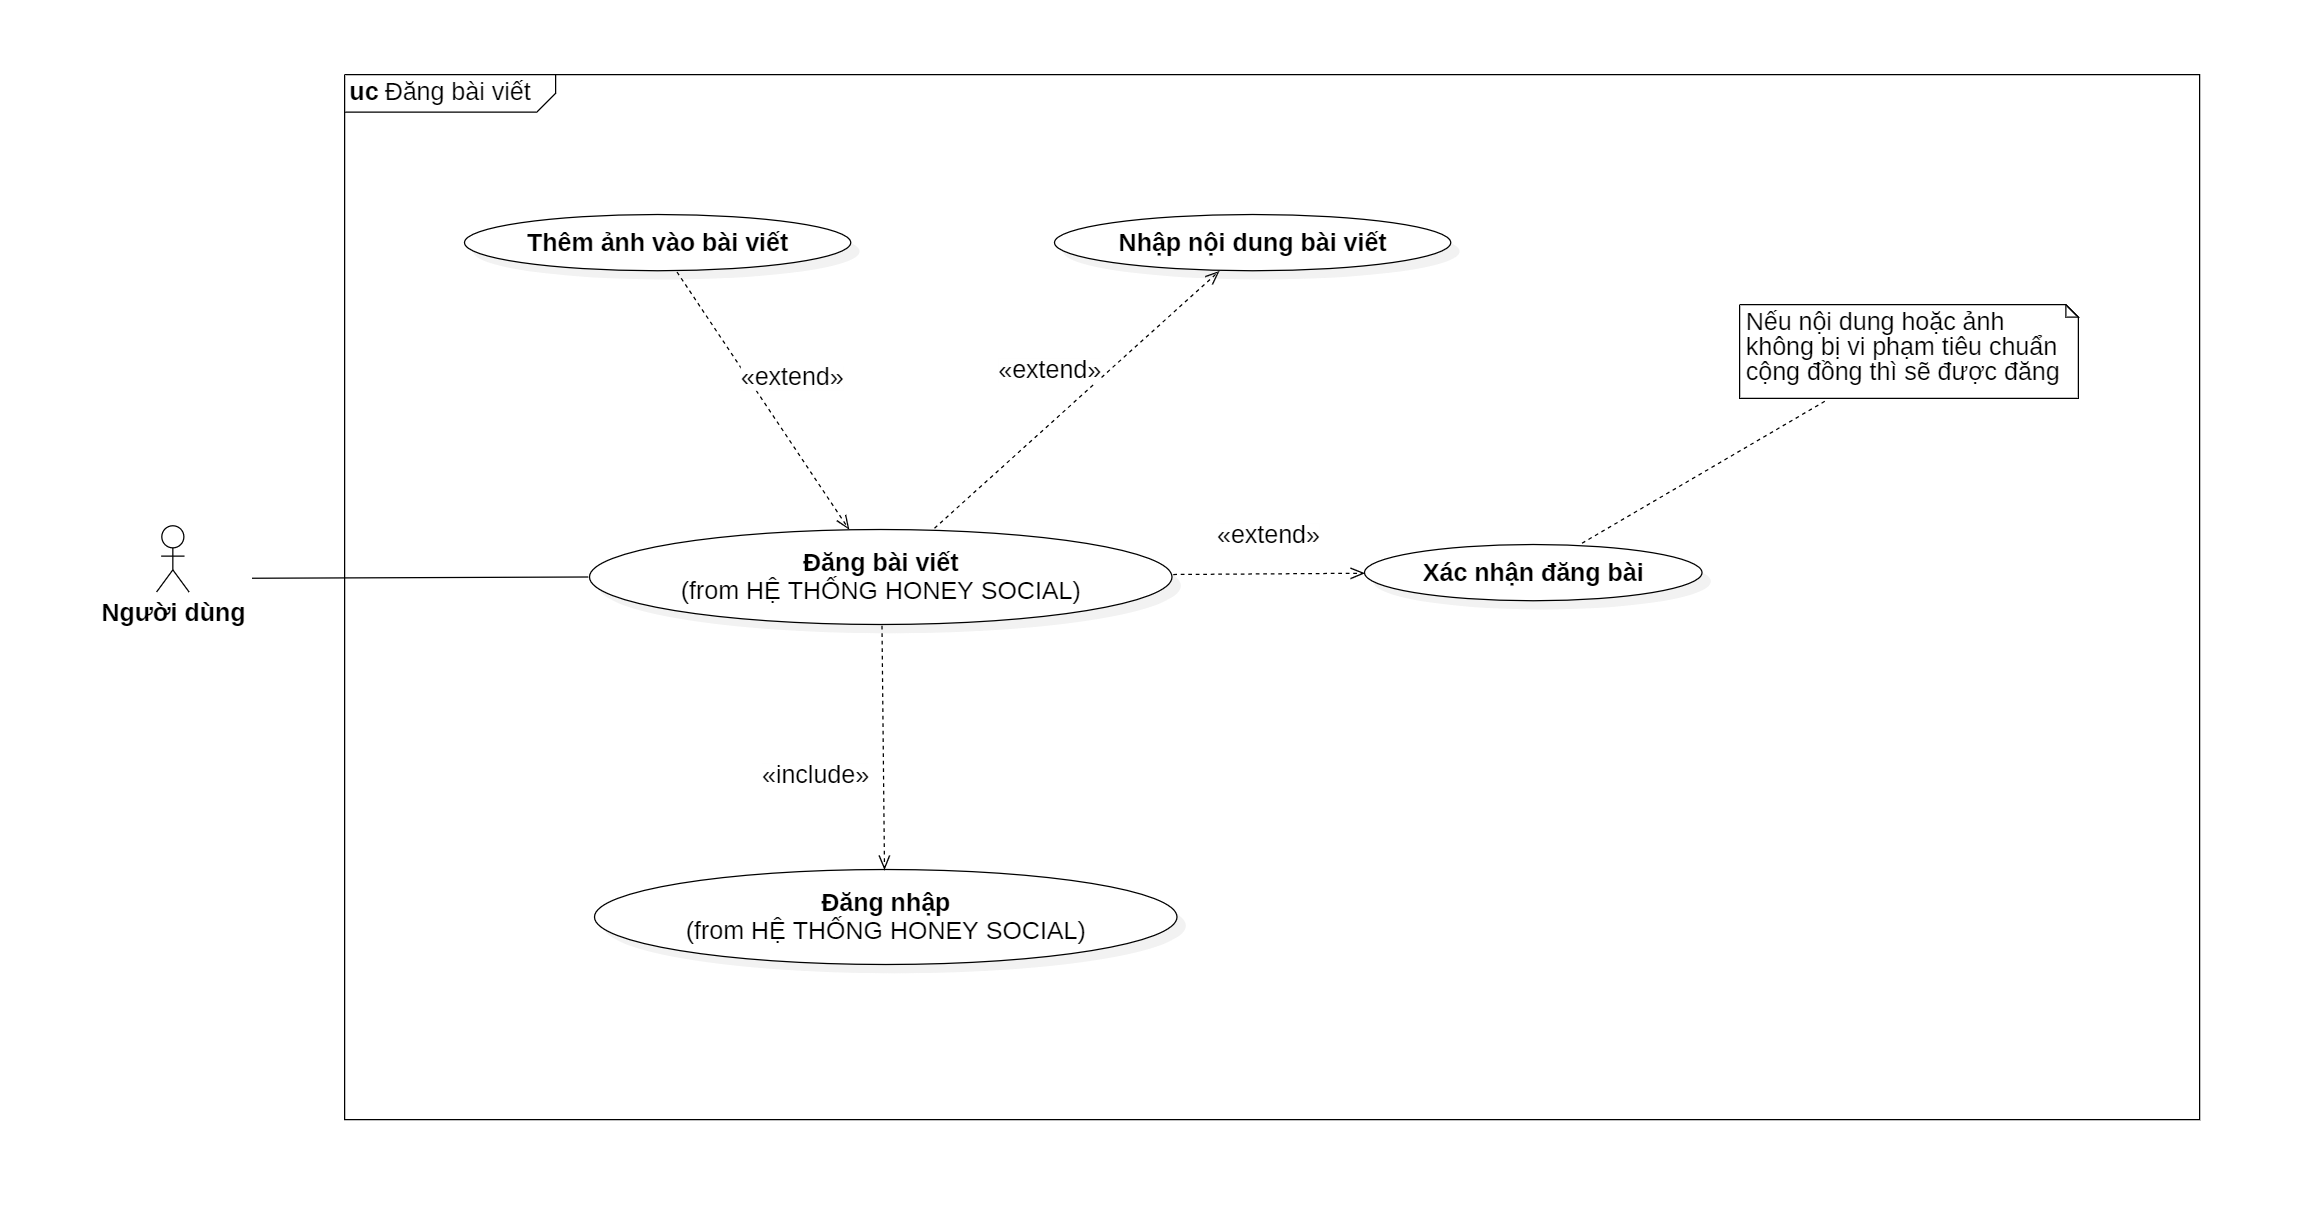
\includegraphics[width=1\textwidth]{image/MoHinh/2.png}
%     \caption{Hình ảnh Đăng bài viết}
%     \label{fig:dang_bai_viet}
% \end{figure}
% Mô tả chi tiết quy trình đăng bài, bắt đầu từ việc người dùng nhập nội dung văn bản, tải lên ảnh hoặc video, chỉnh sửa trước khi đăng (bao gồm thêm hashtag hoặc thẻ người), trải qua kiểm duyệt tự động bằng AI, và cuối cùng là xác nhận để bài viết được công khai trên bảng tin.

% \textbf{Tìm kiếm nâng cao} \\
% \begin{figure}[H]
%     \centering
%     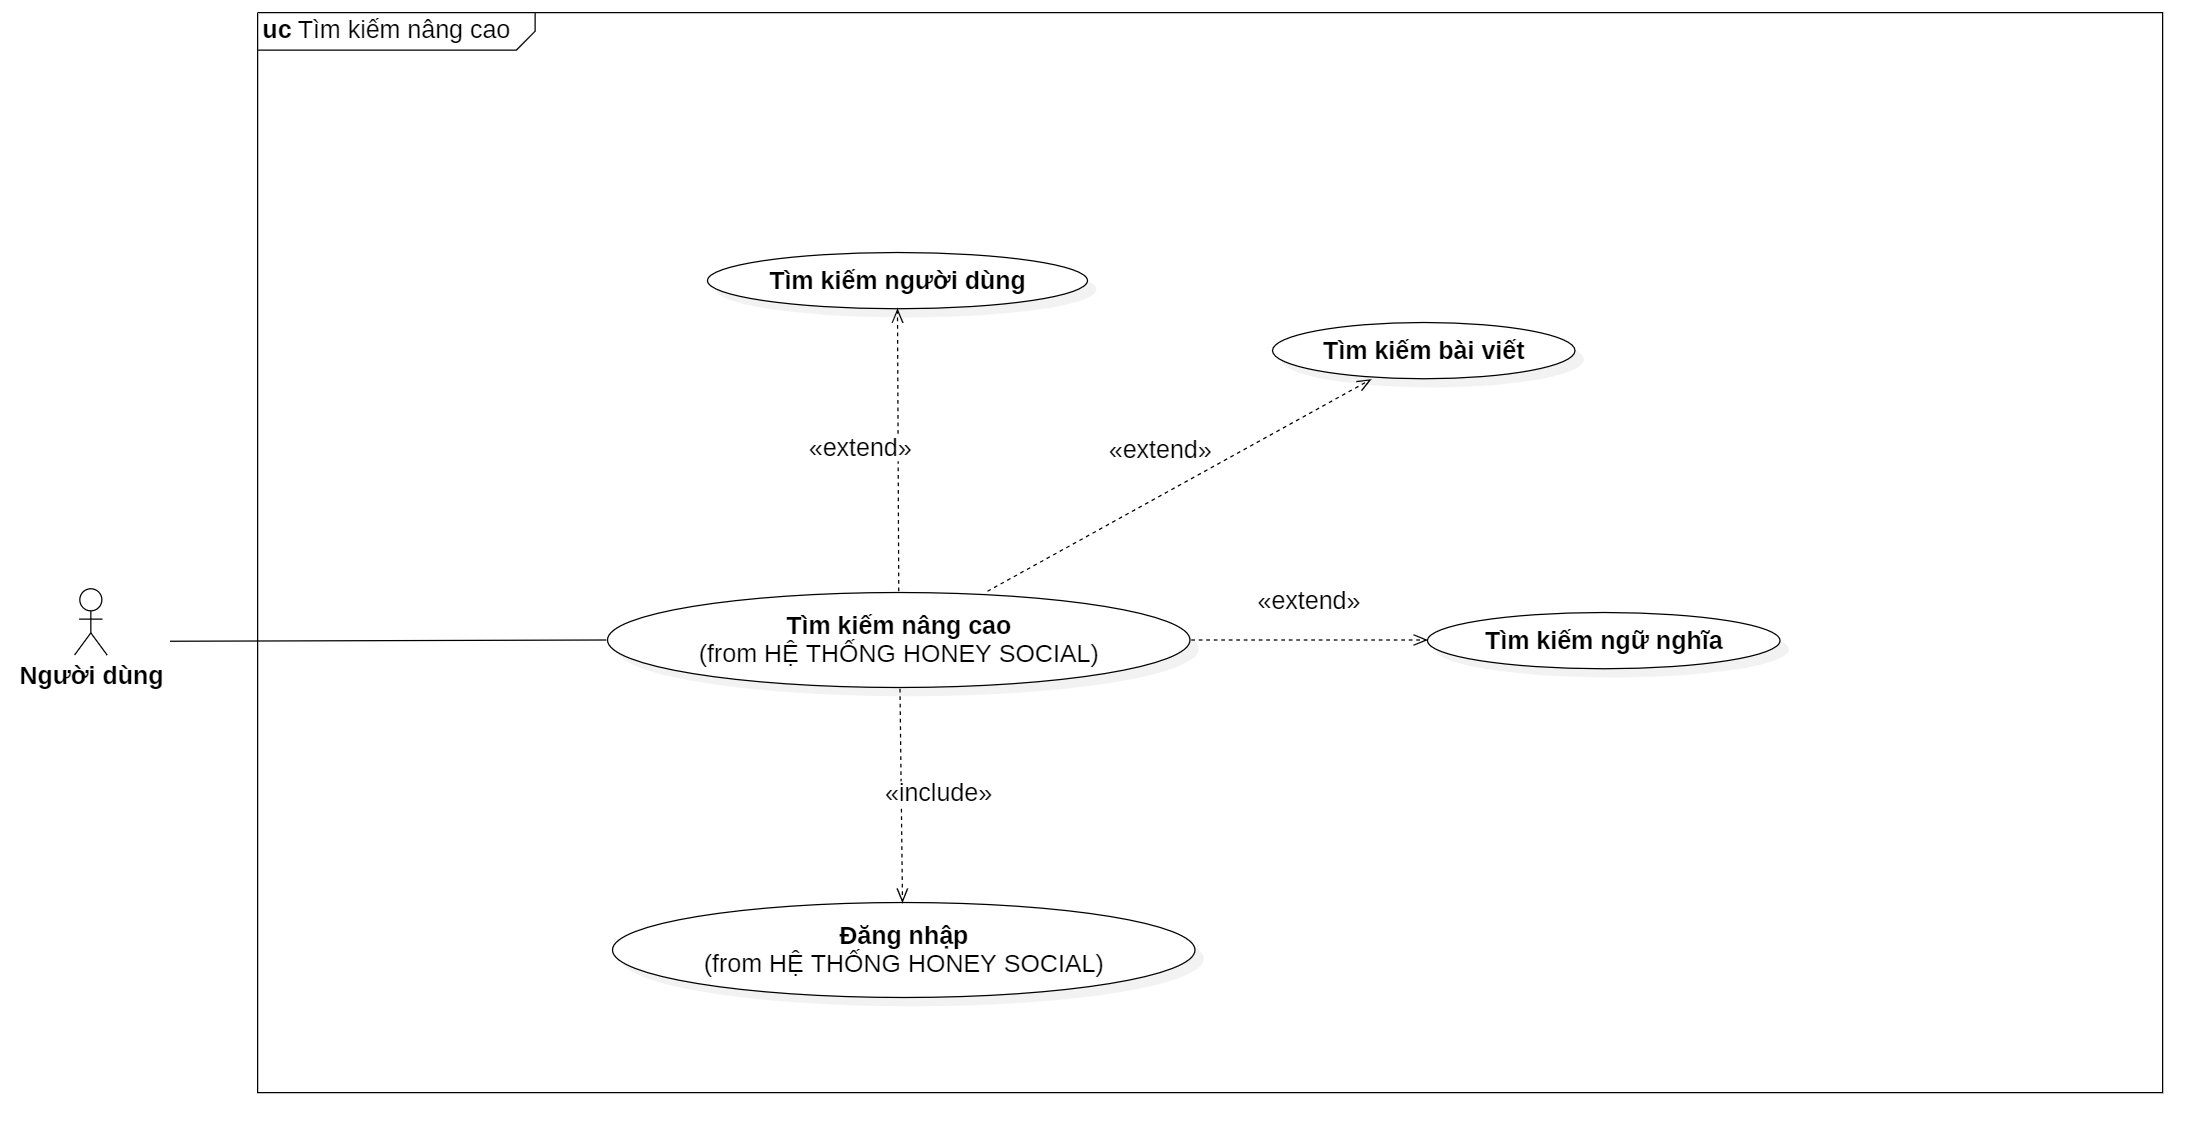
\includegraphics[width=1\textwidth]{image/MoHinh/3.png}
%     \caption{Hình ảnh Tìm kiếm nâng cao}
%     \label{fig:tim_kiem_nang_cao}
% \end{figure}
% Hiển thị quy trình tìm kiếm thông minh, cho phép người dùng sử dụng bộ lọc theo từ khóa, thời gian, hoặc sở thích cá nhân, tích hợp gợi ý dựa trên vector similarity từ Elasticsearch, và sắp xếp kết quả theo mức độ liên quan hoặc thời gian đăng tải để tối ưu hóa trải nghiệm tìm kiếm.

% \newpage
% \textbf{Thông báo} \\
% \begin{figure}[H]
%     \centering
%     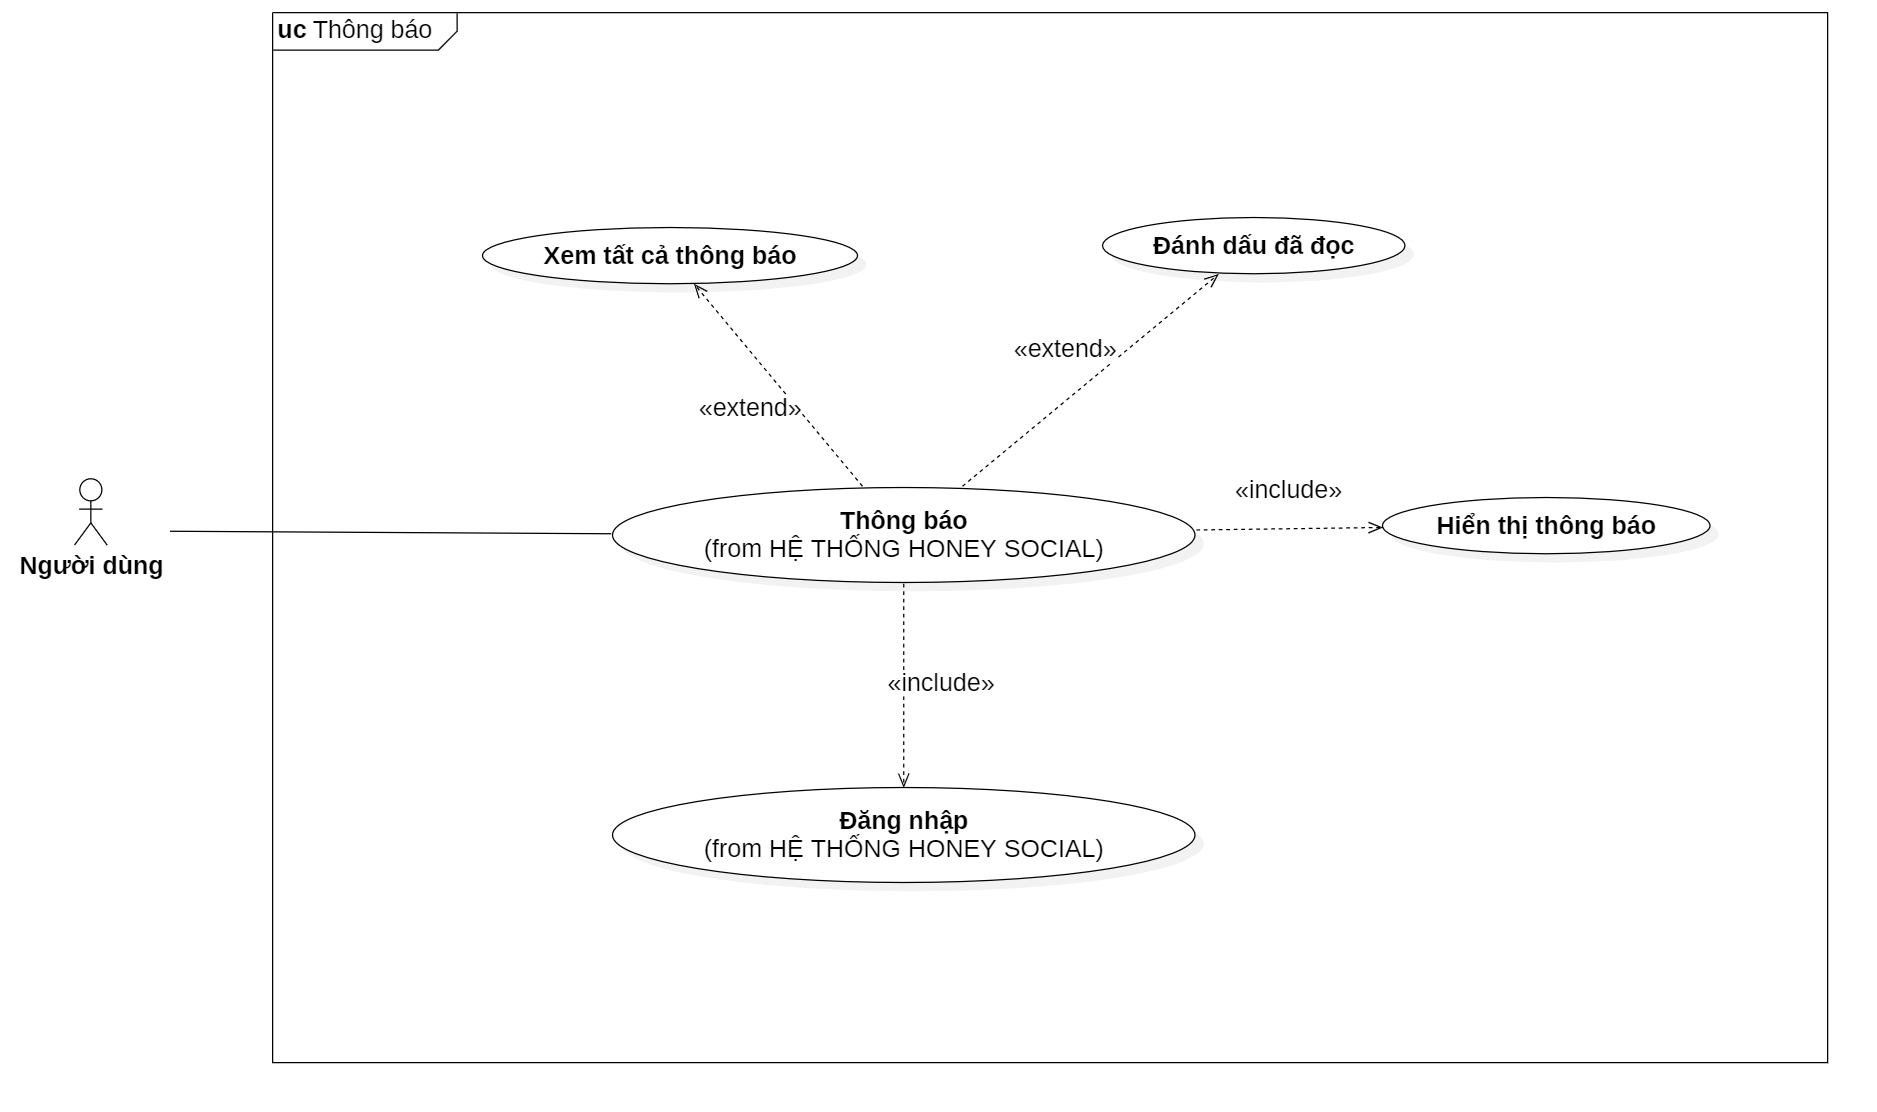
\includegraphics[width=1\textwidth]{image/MoHinh/4.png}
%     \caption{Hình ảnh Thông báo}
%     \label{fig:thong_bao}
% \end{figure}
% Chi tiết hóa cách hệ thống gửi thông báo thời gian thực, bao gồm thông báo khi có tương tác (thích, bình luận), cập nhật từ người theo dõi, hoặc thông báo hệ thống (như xác nhận email), với tùy chọn tắt/mở thông báo để cá nhân hóa trải nghiệm.

% \newpage
% \textbf{Xem hồ sơ người dùng} \\
% \begin{figure}[H]
%     \centering
%     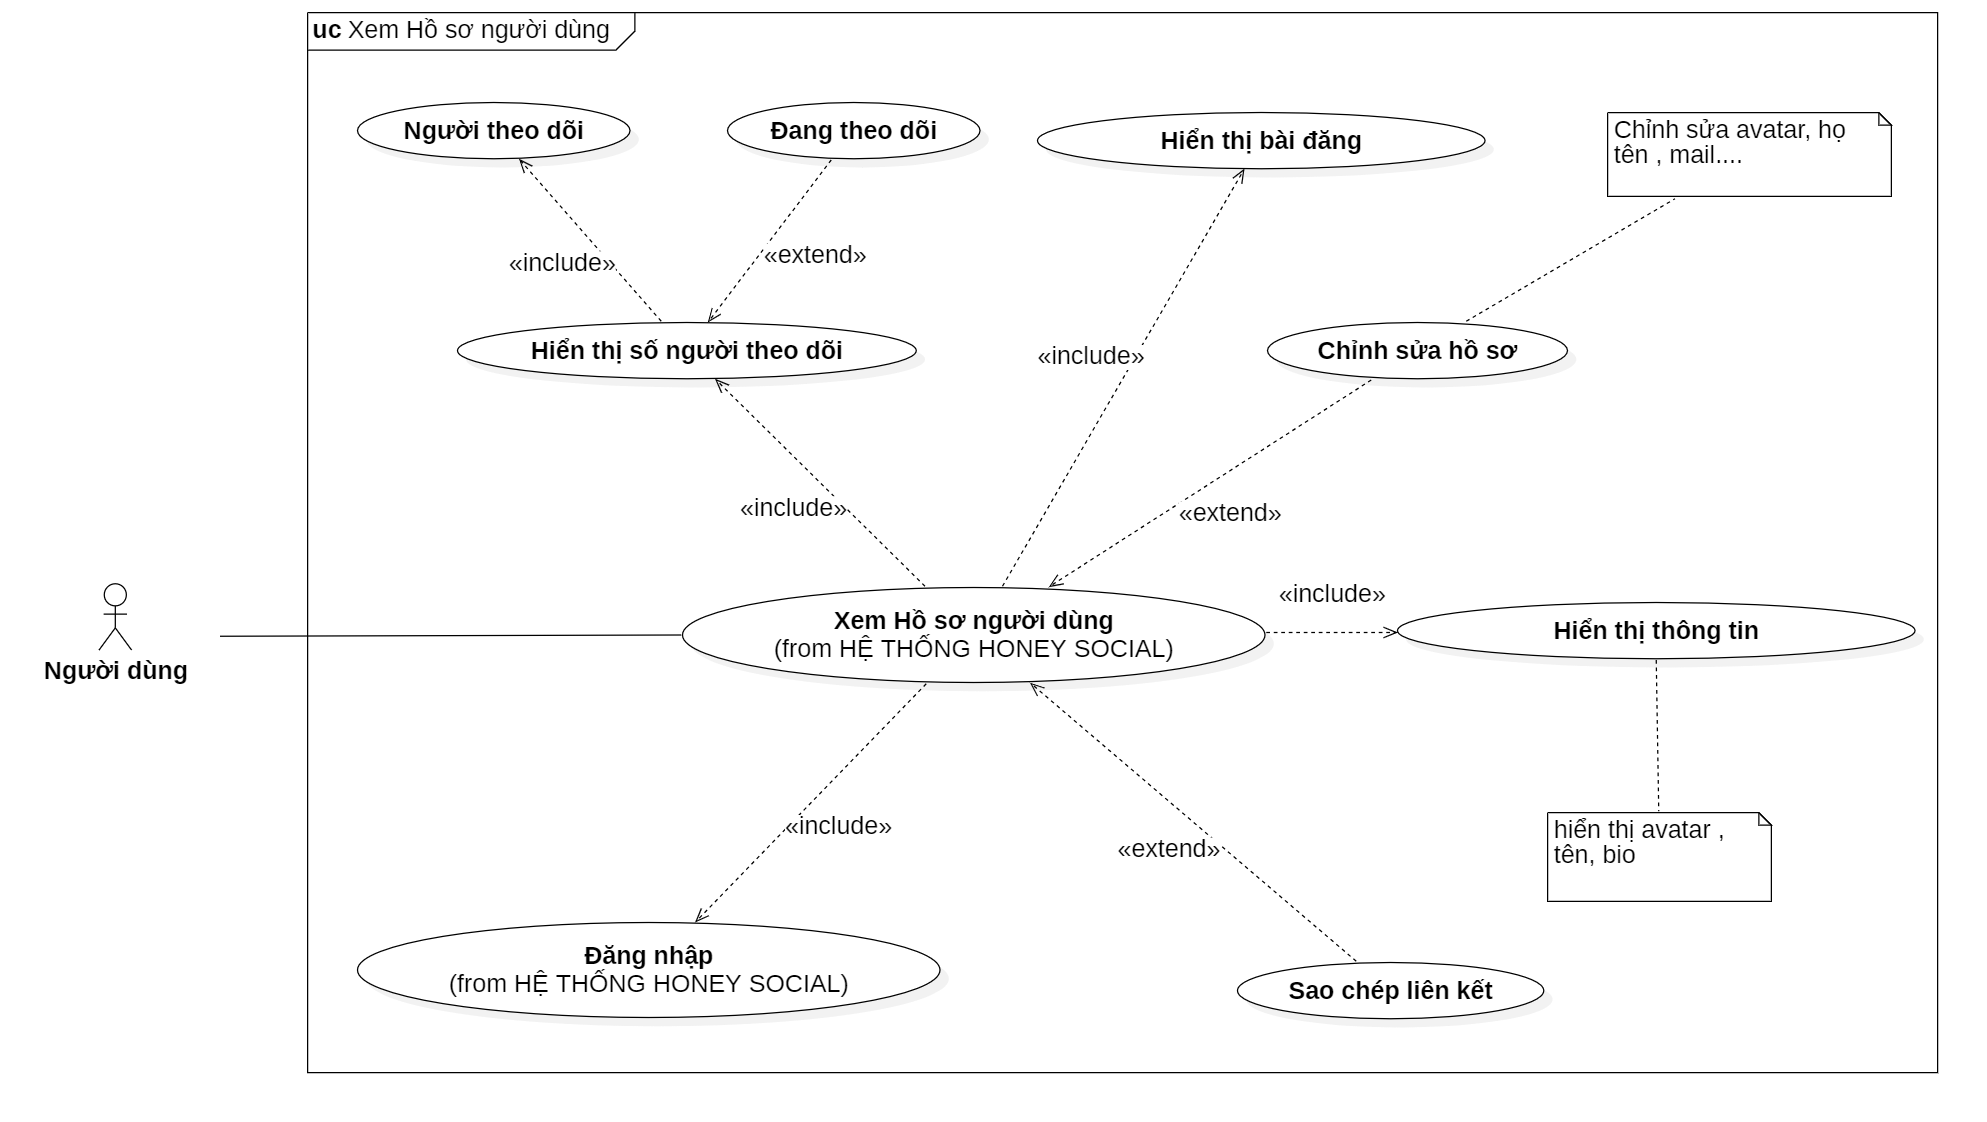
\includegraphics[width=1\textwidth]{image/MoHinh/5.png}
%     \caption{Hình ảnh Xem Hồ sơ người dùng}
%     \label{fig:xem_ho_so_nguoi_dung}
% \end{figure}
% Hướng dẫn chi tiết cách người dùng xem và chỉnh sửa hồ sơ cá nhân, bao gồm cập nhật avatar thông qua Cloudinary, chỉnh sửa thông tin như tên, bio, và danh sách theo dõi/người theo dõi, cùng với các thống kê cơ bản như số bài đăng.

% \textbf{Báo cáo bài viết} \\
% \begin{figure}[H]
%     \centering
%     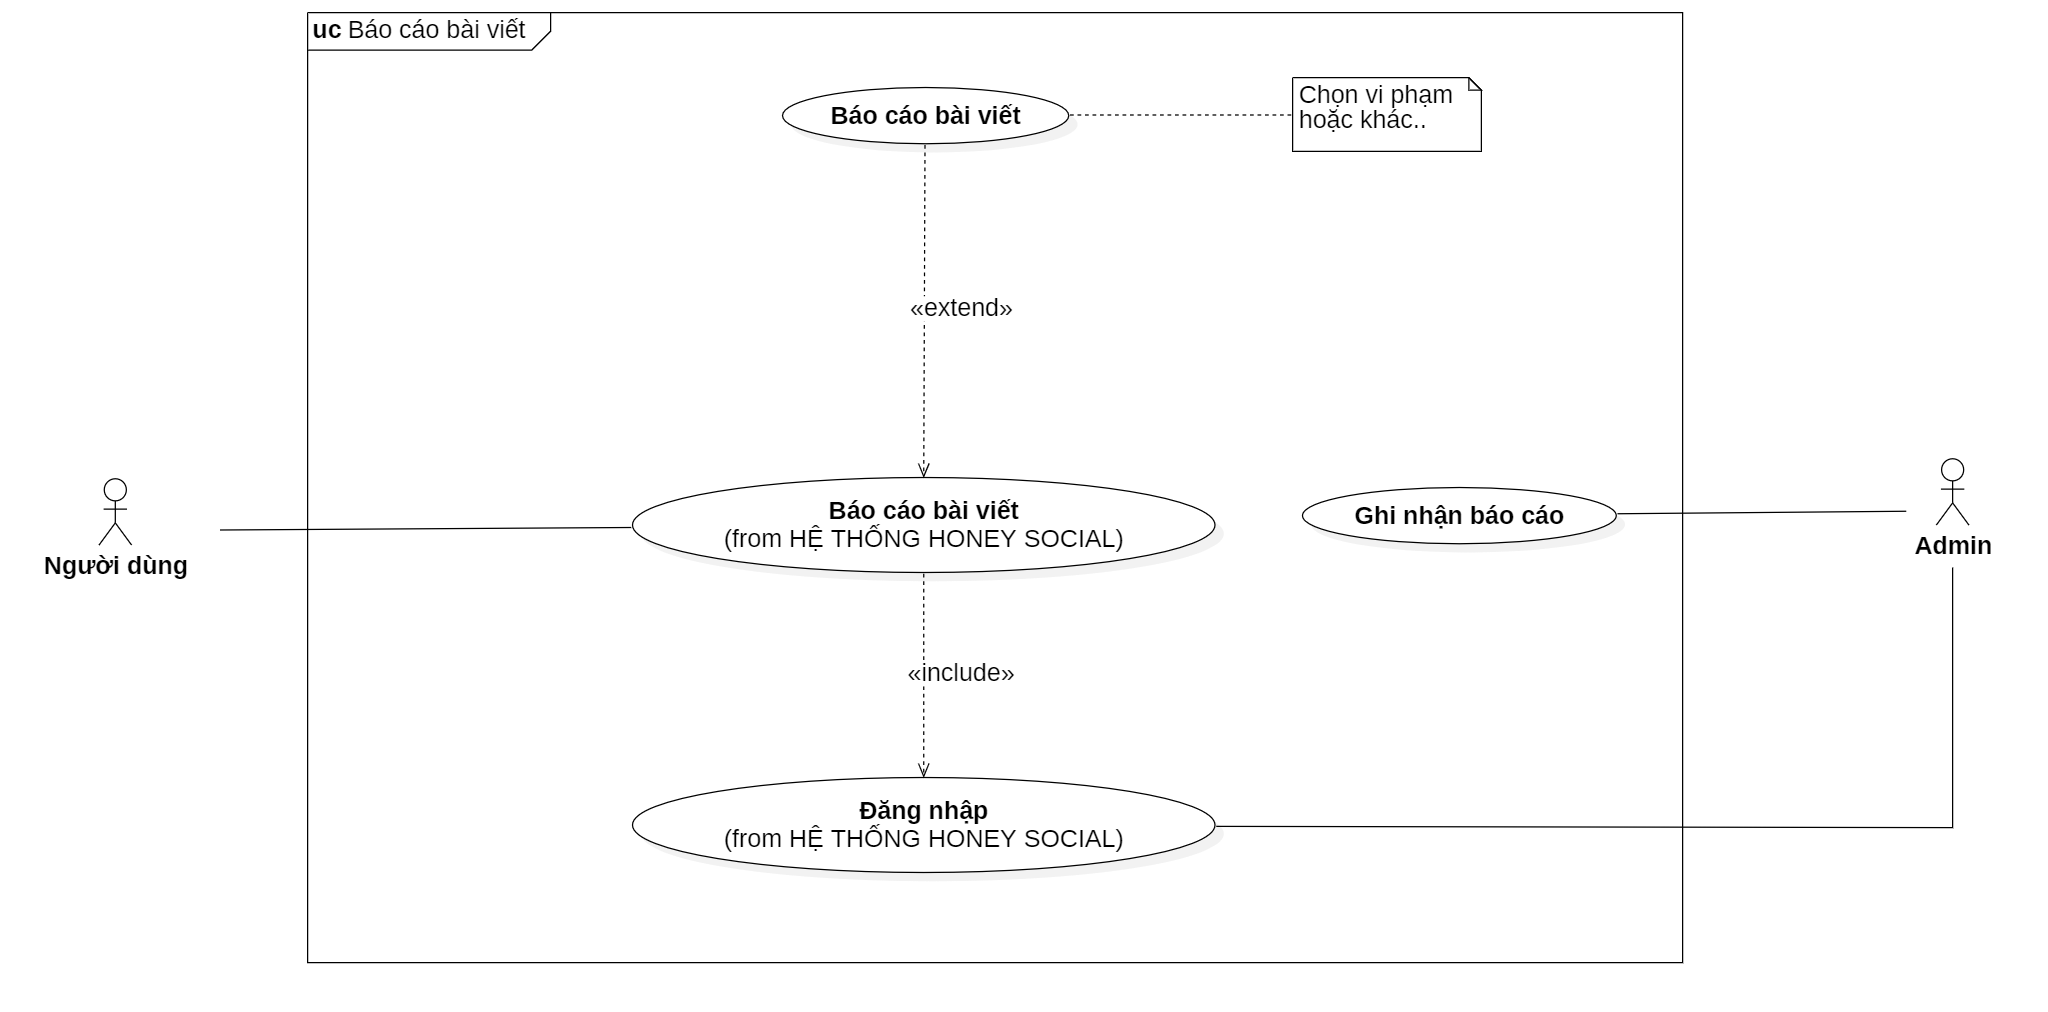
\includegraphics[width=1\textwidth]{image/MoHinh/6.png}
%     \caption{Hình ảnh Báo cáo bài viết}
%     \label{fig:bao_cao_bai_viet}
% \end{figure}
% Mô tả quy trình người dùng báo cáo vi phạm, bao gồm chọn lý do cụ thể (nội dung không phù hợp, bạo lực, spam...), gửi thông tin kèm bằng chứng qua API, và chuyển đến quản trị viên để xử lý theo các cấp độ (nhẹ, vừa, nặng).

% \textbf{Trò chuyện AI} \\
% \begin{figure}[H]
%     \centering
%     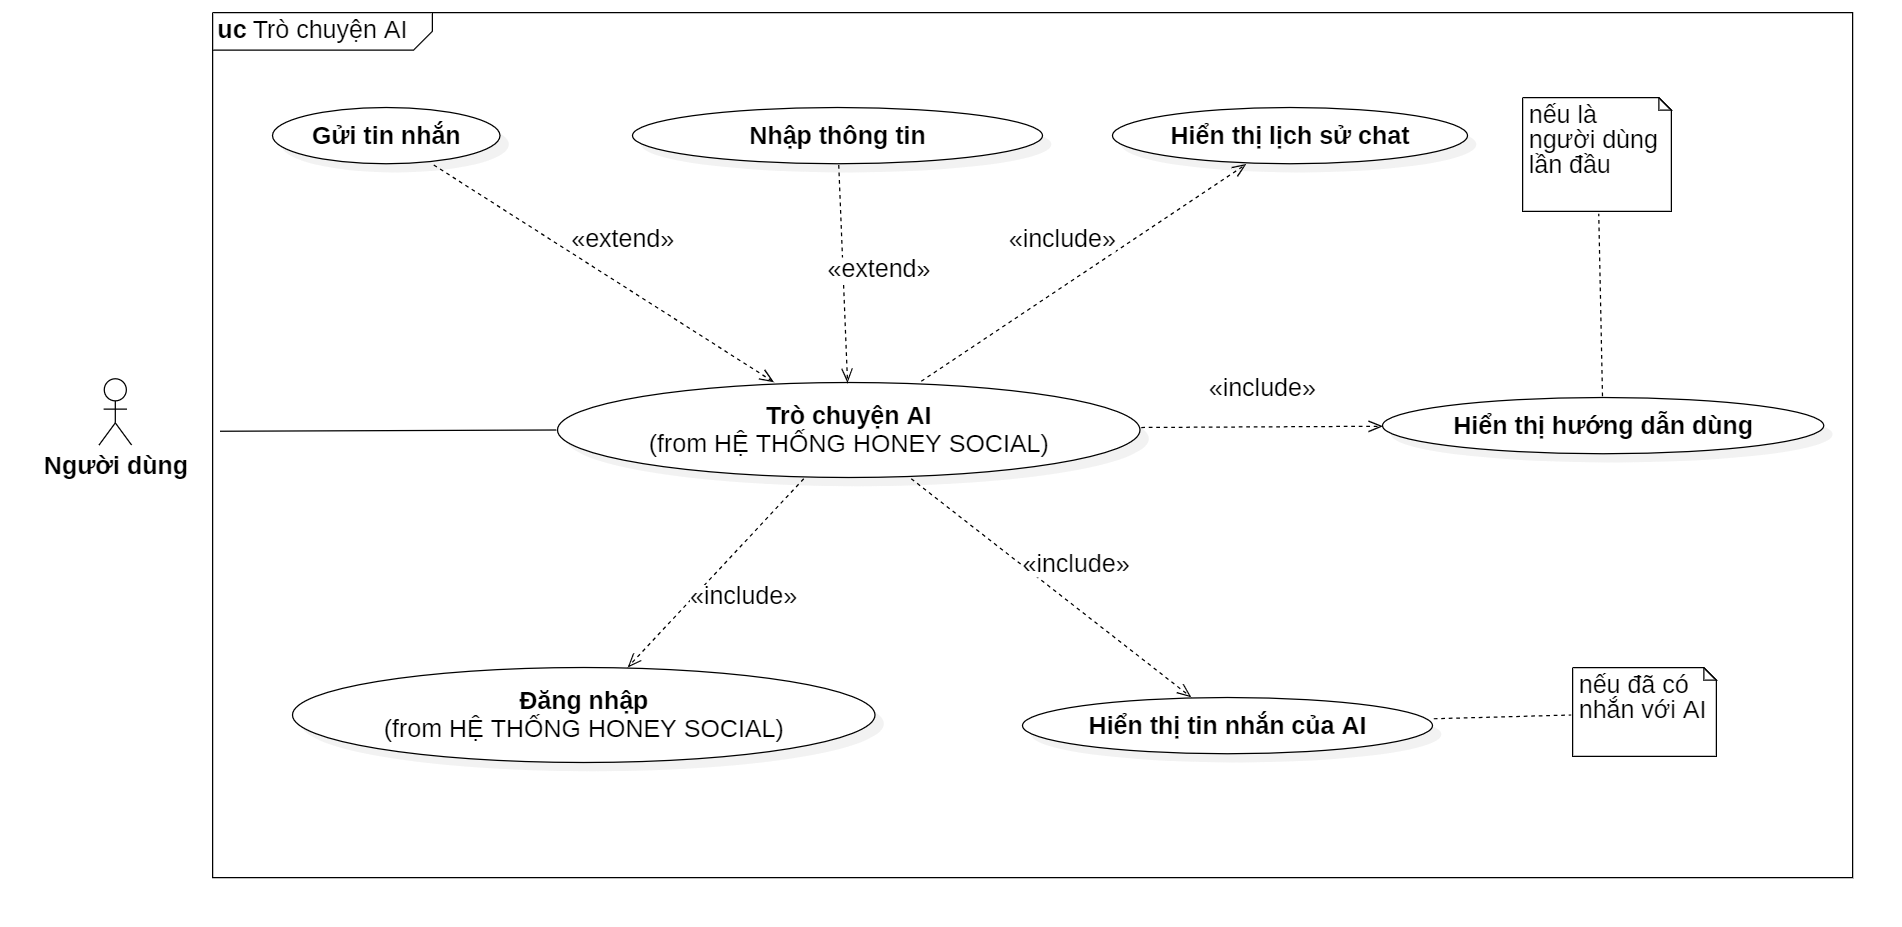
\includegraphics[width=1\textwidth]{image/MoHinh/7.png}
%     \caption{Hình ảnh Trò chuyện AI}
%     \label{fig:tro_chuyen_ai}
% \end{figure}
% Phác thảo chức năng chat AI, hỗ trợ trả lời câu hỏi liên quan đến nội dung bài viết, gợi ý bài viết dựa trên sở thích, và tự động phát hiện/phân loại báo cáo vi phạm, với giao diện thân thiện và phản hồi thời gian thực.

% \newpage
% \textbf{Xem bảng tin} \\
% \begin{figure}[H]
%     \centering
%     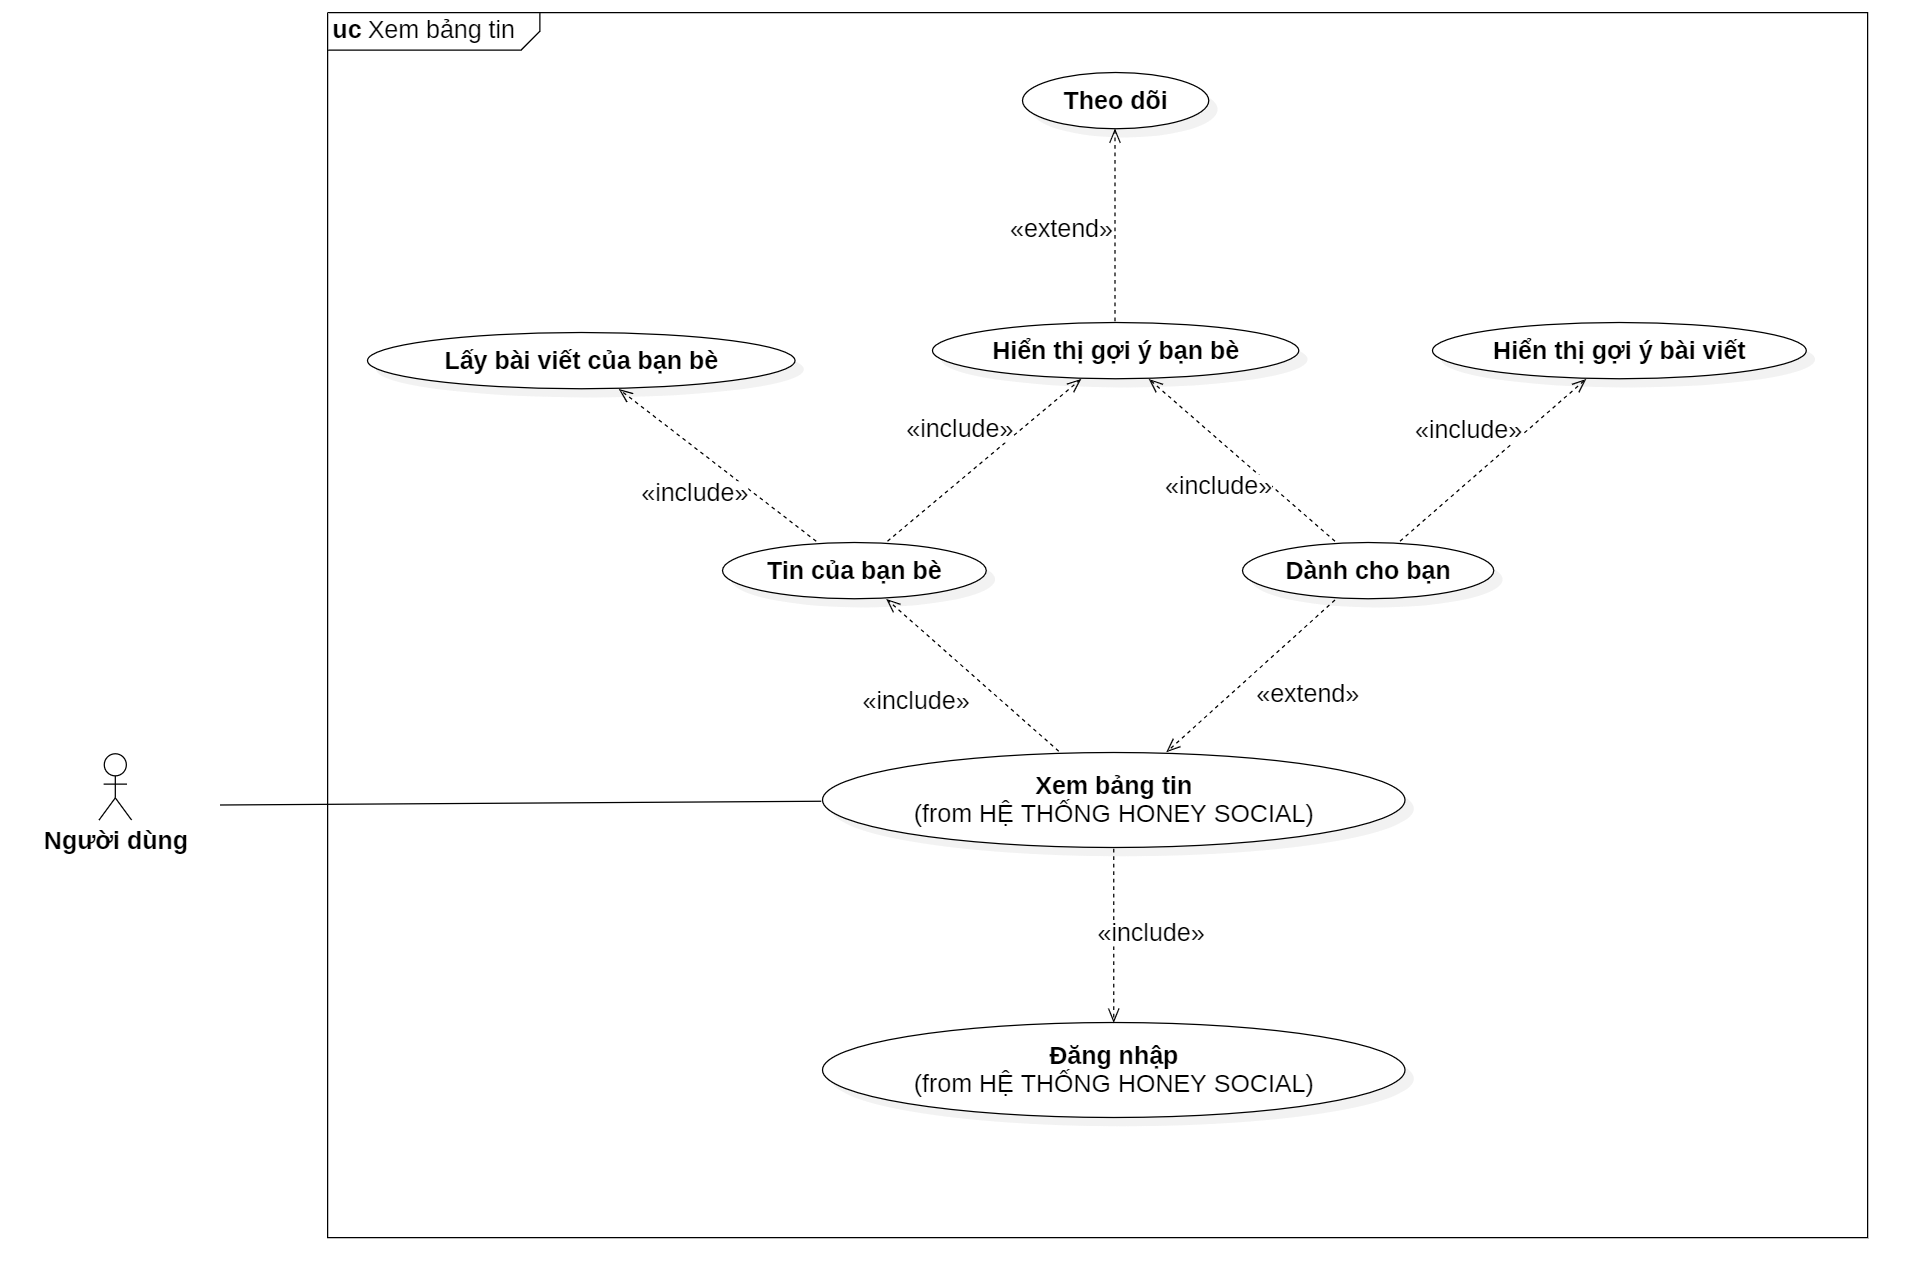
\includegraphics[width=1\textwidth]{image/MoHinh/8.png}
%     \caption{Hình ảnh Xem bảng tin}
%     \label{fig:xem_bang_tin}
% \end{figure}
% Thể hiện cách hệ thống hiển thị feed bài viết cá nhân hóa, lấy dữ liệu từ người dùng theo dõi, tích hợp gợi ý từ AI dựa trên vector nhúng, và cho phép làm mới feed hoặc lọc theo chủ đề để tăng tính tương tác.

% \textbf{Xem hồ sơ người khác} \\
% \begin{figure}[H]
%     \centering
%     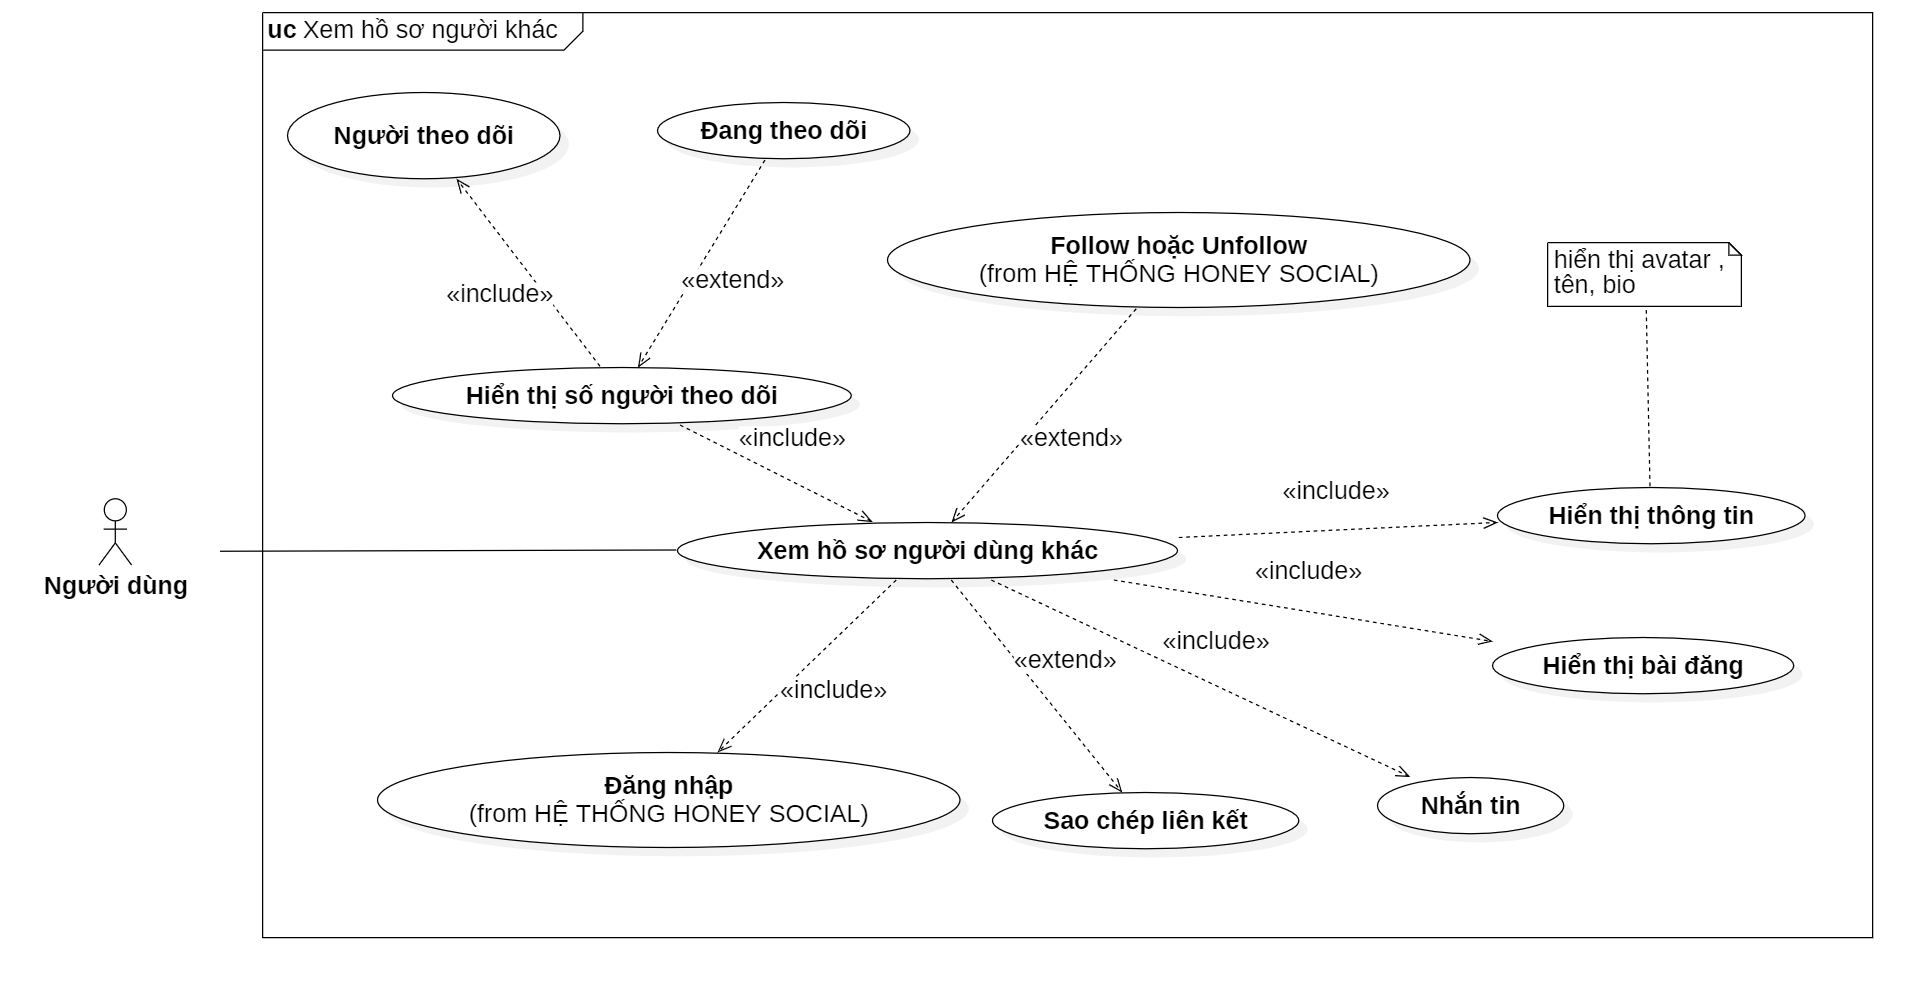
\includegraphics[width=1\textwidth]{image/MoHinh/9.png}
%     \caption{Hình ảnh Xem hồ sơ người khác}
%     \label{fig:xem_ho_so_nguoi_khac}
% \end{figure}
% Chi tiết quy trình xem hồ sơ người dùng khác, bao gồm thông tin cơ bản (tên, avatar, bio), danh sách bài đăng công khai, và các tùy chọn tương tác như theo dõi hoặc gửi tin nhắn.

% \textbf{Đăng ký} \\
% \begin{figure}[H]
%     \centering
%     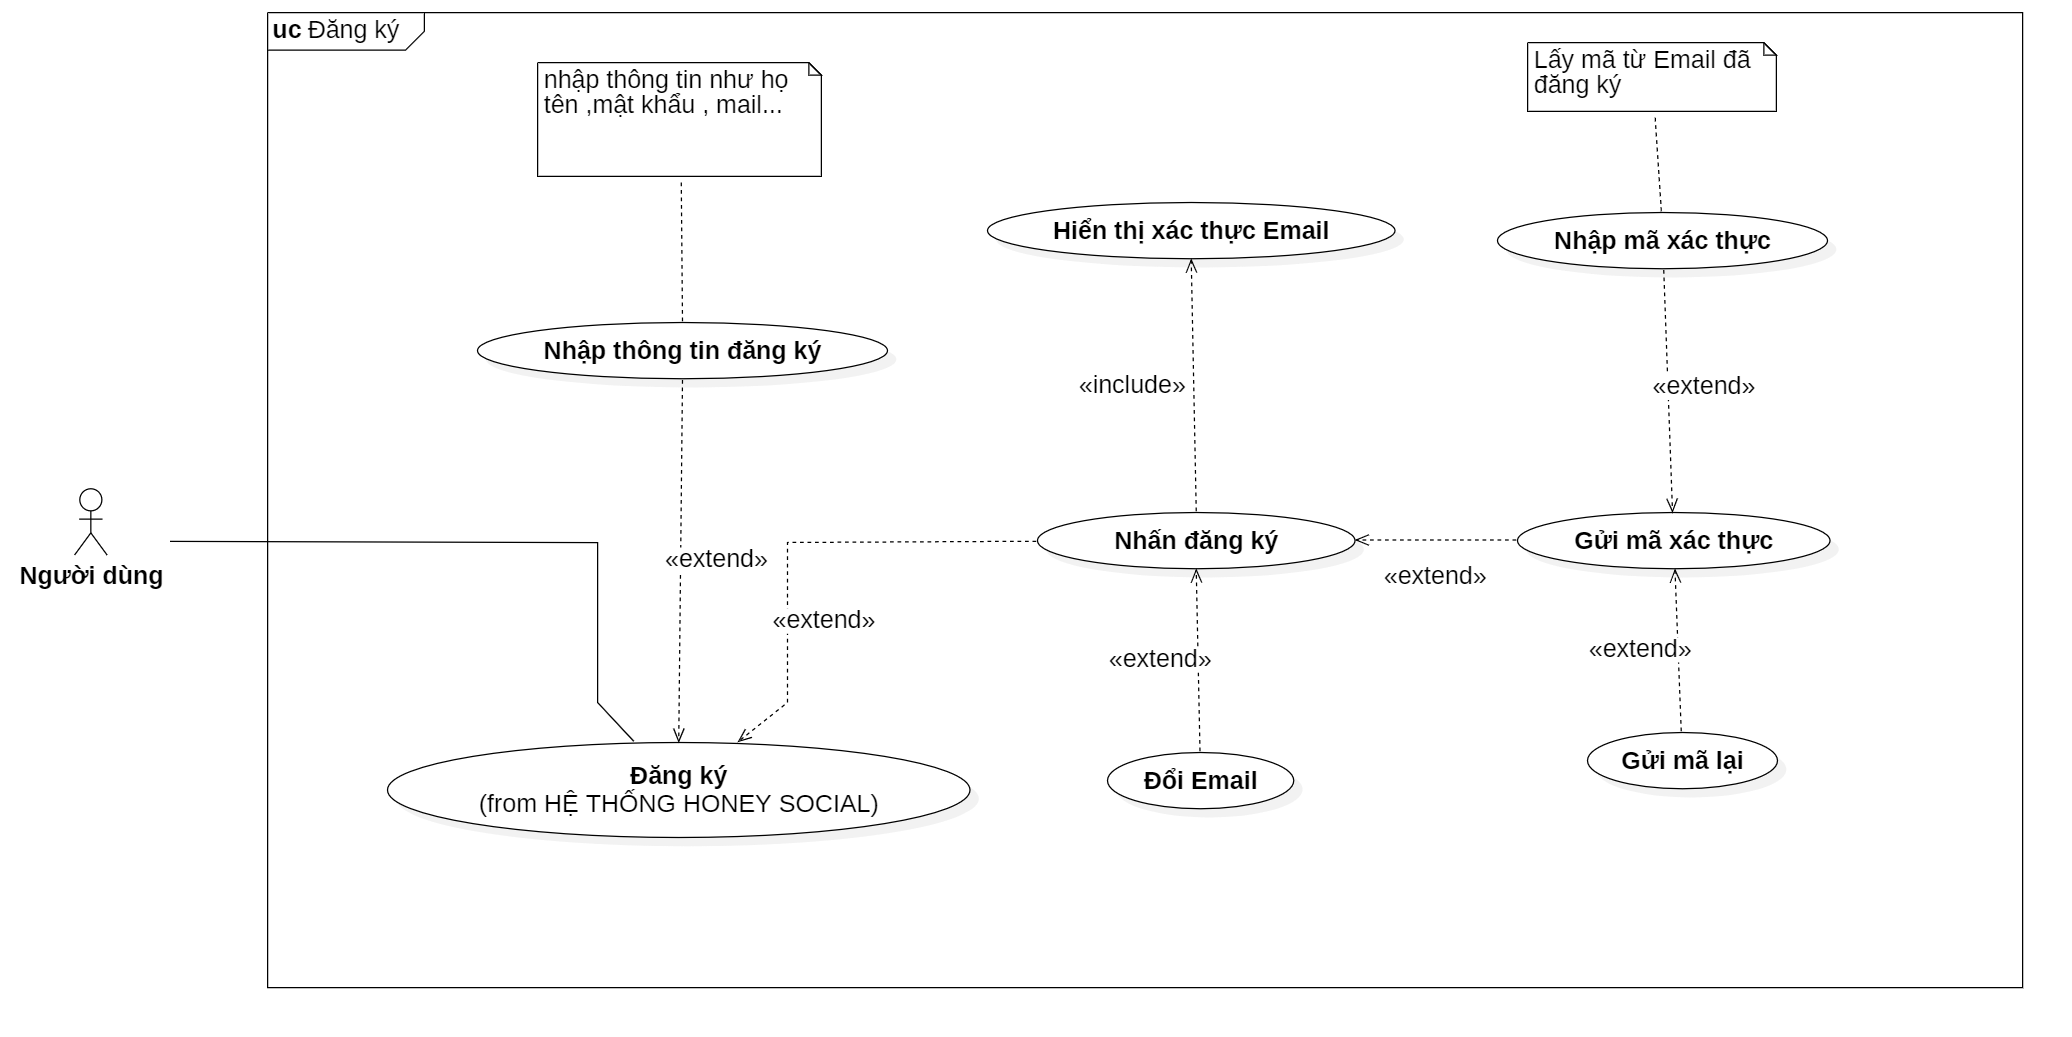
\includegraphics[width=1\textwidth]{image/MoHinh/10.png}
%     \caption{Hình ảnh Đăng ký}
%     \label{fig:dang_ky}
% \end{figure}
% Mô tả quy trình đăng ký tài khoản, yêu cầu nhập thông tin (email, mật khẩu), gửi mã OTP qua Resend API để xác thực, và hoàn tất với tùy chọn cá nhân hóa hồ sơ ngay sau đăng ký.
% \newpage
% \textbf{Quản lý nội dung báo cáo} \\
% \begin{figure}[H]
%     \centering
%     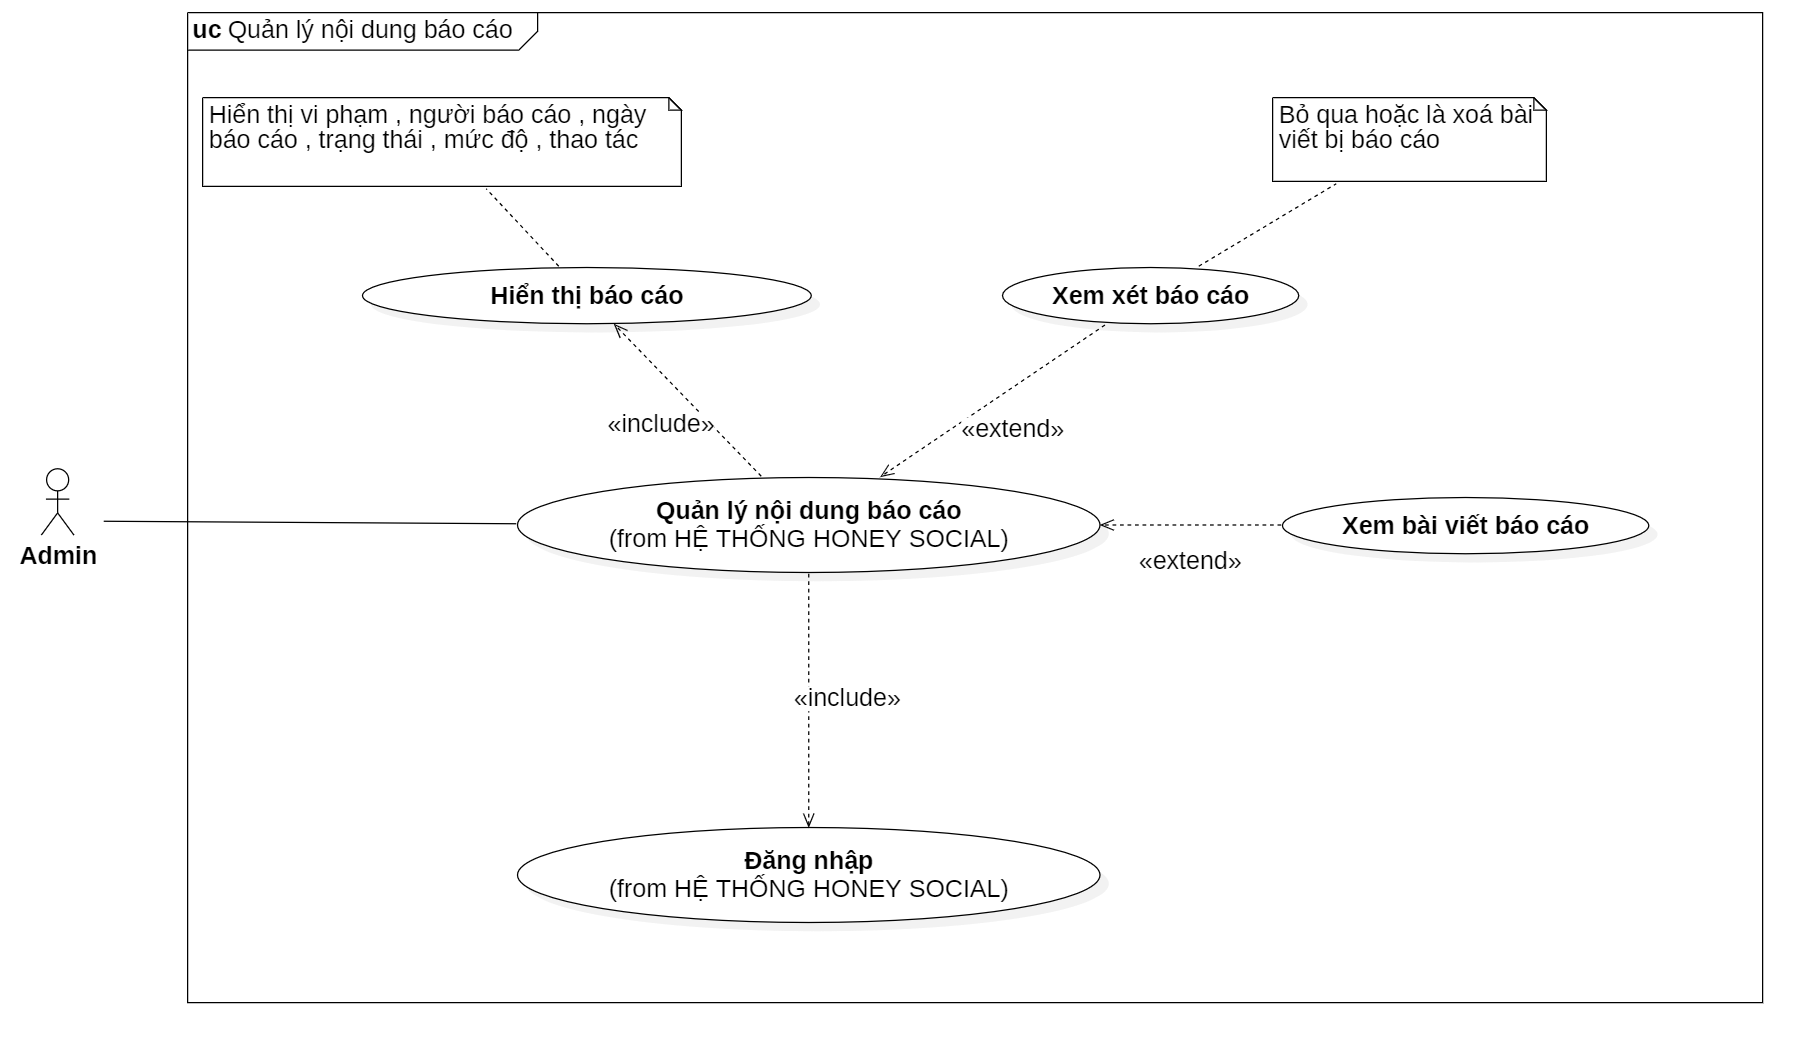
\includegraphics[width=1\textwidth]{image/MoHinh/11.png}
%     \caption{Hình ảnh Quản lý nội dung báo cáo}
%     \label{fig:quan_ly_noi_dung_bao_cao}
% \end{figure}
% Hiển thị cách quản trị viên tiếp nhận báo cáo từ người dùng, phân loại theo mức độ vi phạm (nhẹ: cảnh báo; vừa: ẩn bài; nặng: xóa và khóa tài khoản), và xử lý qua dashboard admin với các công cụ lọc theo thời gian hoặc lý do.
% \newpage
% \textbf{Tương tác bài viết} \\
% \begin{figure}[H]
%     \centering
%     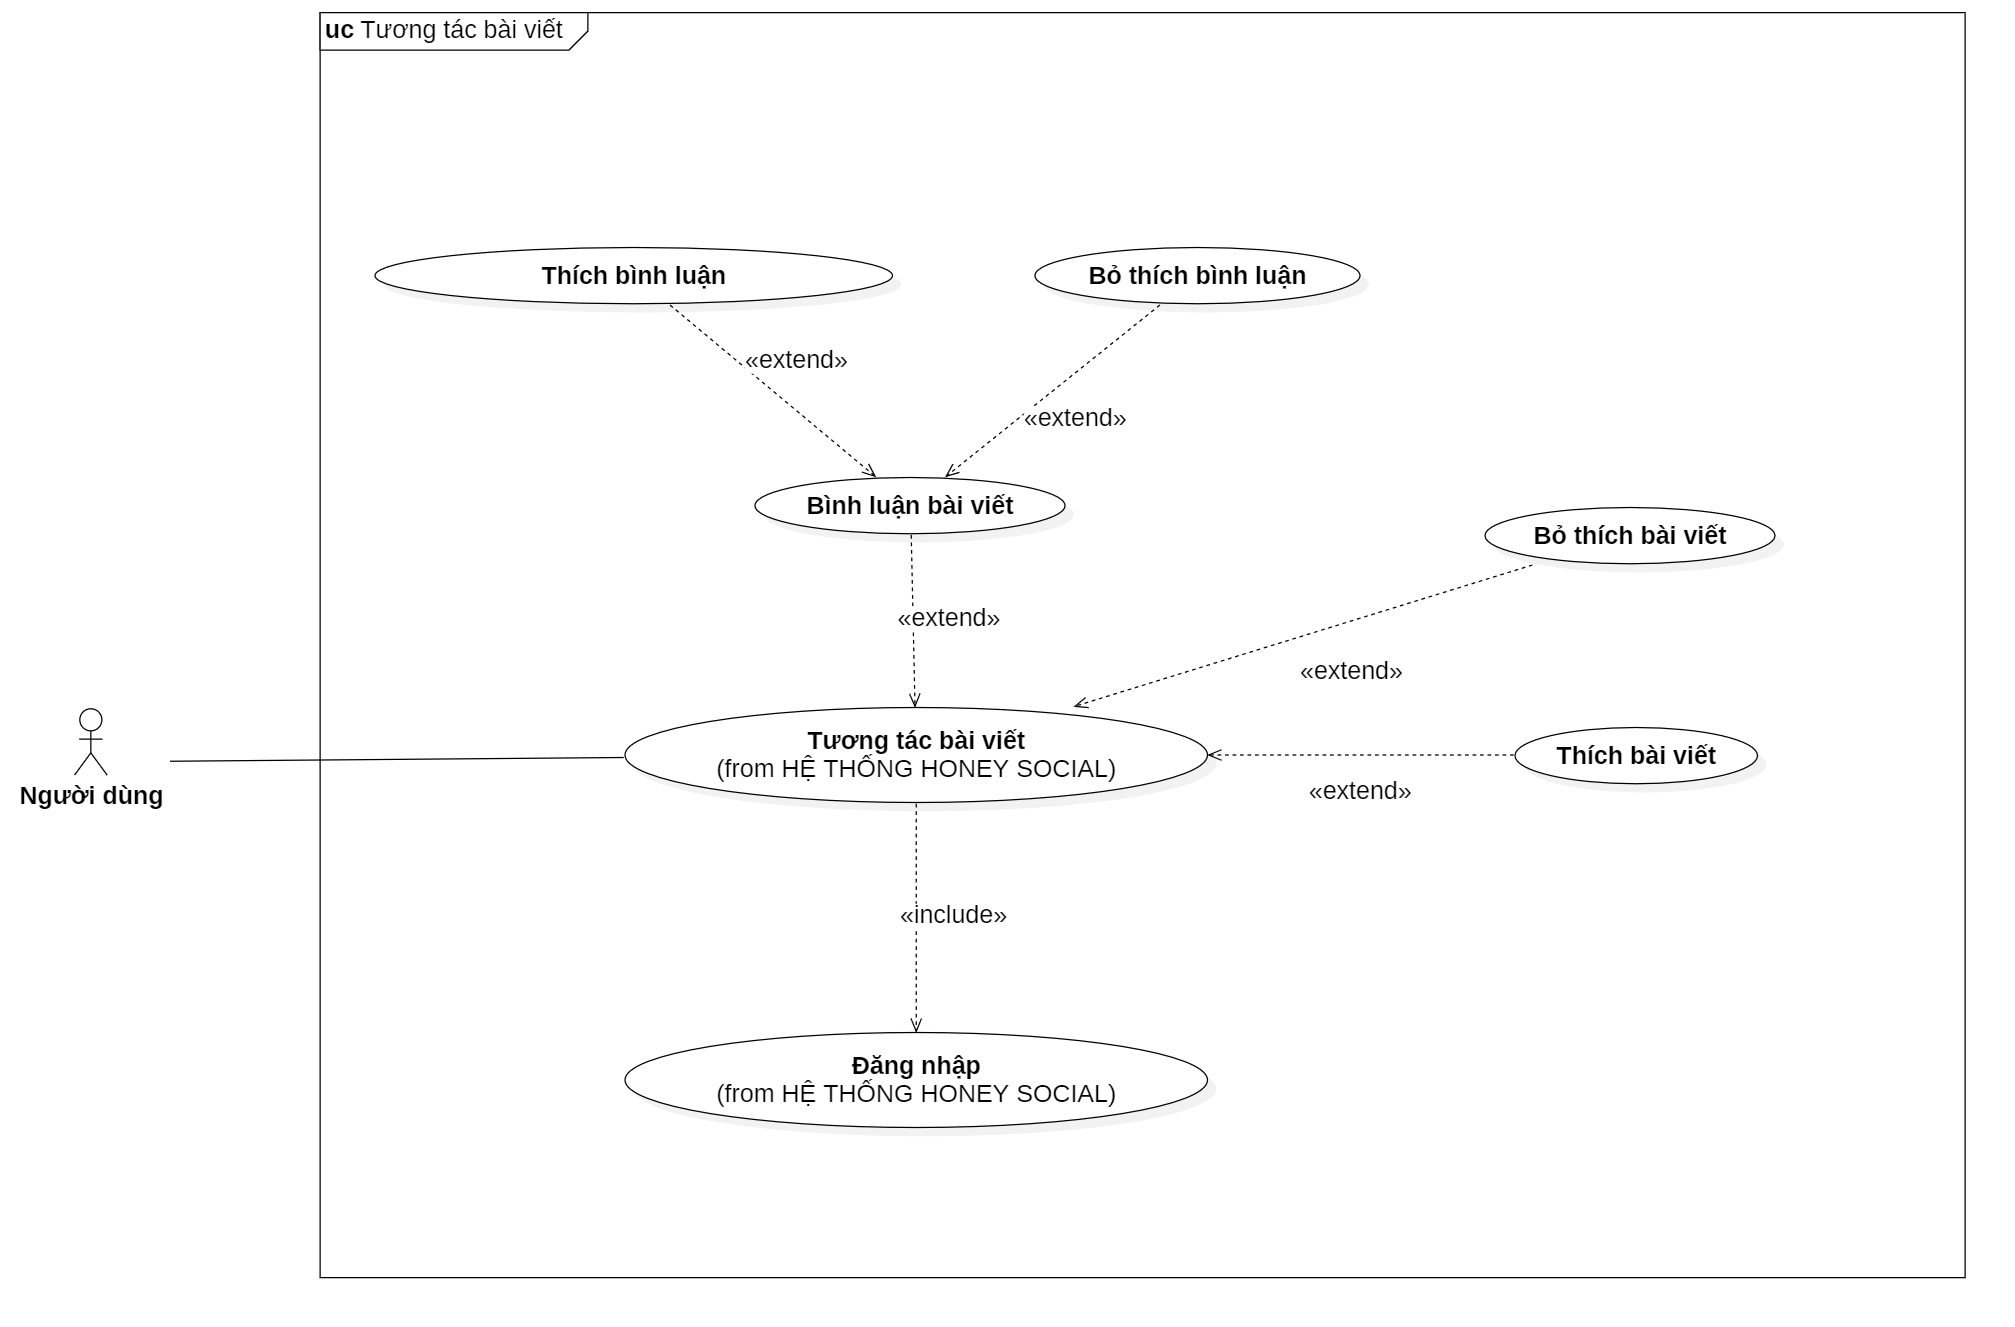
\includegraphics[width=1\textwidth]{image/MoHinh/12.png}
%     \caption{Hình ảnh Tương tác bài viết}
%     \label{fig:tuong_tac_bai_viet}
% \end{figure}
% Phác thảo các hành động tương tác như thích (like), bình luận (với khả năng phản hồi), và chia sẻ liên kết bài viết ra ngoài, tất cả đều được xử lý qua Socket.IO để đảm bảo cập nhật thời gian thực.

% \newpage

% \subsubsection{Kịch bản của các UseCase}


% \begin{longtable}{|>{\bfseries}m{4cm}|m{10cm}|}
% \caption{Bảng thông tin hoạt động của chức năng đăng bài viết}
% \label{table:usecase-posts}\\
% \hline
% Use-case name & Đăng bài viết \\ 
% \hline 
% Description & Người dùng đăng một bài viết mới lên hệ thống, có thể kèm hình ảnh.\\
% \hline
% Actor & Người dùng đã đăng nhập\\
% \hline
% Pre-Conditions & -Người dùng đã đăng nhập vào hệ thống.

% -Email của người dùng đã được xác thực (nếu hệ thống yêu cầu).\\
% \hline
% Post-Condition & -Bài viết mới được lưu vào hệ thống và hiển thị trên bảng tin.

% -Nếu có lỗi, thông báo lỗi được hiển thị cho người dùng.\\
% \hline
% Trigger & Người dùng nhấn nút "Tạo bài viết mới" hoặc biểu tượng "+".\\
% \hline
% Normal Flow &
% \begin{enumerate}
%     \item Người dùng nhấn nút "Tạo bài viết mới".
%     \item Hệ thống hiển thị modal nhập nội dung bài viết.
%     \item Người dùng nhập nội dung, chọn hình ảnh (nếu muốn).
%     \item Người dùng nhấn nút "Đăng".
%     \item Hệ thống kiểm tra điều kiện (đăng nhập, xác thực email, nội dung hợp lệ).
%     \item Nếu hợp lệ, bài viết được lưu và hiển thị; thông báo thành công cho người dùng.
% \end{enumerate} \\
% \hline
% Alternative Flow & Nếu người dùng chưa đăng nhập: Hệ thống thông báo và chuyển hướng đến trang đăng nhập.

% Nếu email chưa xác thực: Hệ thống thông báo yêu cầu xác thực email.

% Nếu nội dung vi phạm hoặc lỗi khác: Hệ thống hiển thị thông báo lỗi chi tiết.

% Nếu người dùng nhấn "Hủy": Modal đóng, không lưu bài viết.\\
% \hline
% \end{longtable}


% % \subsubsubsection{Chức năng tìm kiếm nâng cao}
% \begin{longtable}{|>{\bfseries}m{4cm}|m{10cm}|}
% \caption{Bảng thông tin hoạt động của chức năng tìm kiếm nâng cao}
% \label{table:usecase-search}\\
% \hline
% Use-case name & Tìm kiếm nâng cao
% \\
% \hline
% Description & Người dùng thực hiện tìm kiếm nâng cao để tìm kiếm người dùng, bài viết hoặc theo ngữ nghĩa trên hệ thống.\\
% \hline
% Actor & Người dùng đã đăng nhập
% \\
% \hline
% Pre-Conditions & Người dùng đã đăng nhập vào hệ thống.

% Hệ thống có dữ liệu người dùng/bài viết.\\
% \hline
% Post-Condition & Kết quả tìm kiếm được hiển thị cho người dùng theo tiêu chí đã chọn.

% Người dùng có thể chuyển trang, sắp xếp hoặc chọn kết quả để xem chi tiết.\\
% \hline
% Trigger & Người dùng truy cập trang tìm kiếm nâng cao hoặc nhập từ khóa vào ô tìm kiếm.
% \\
% \hline
% Normal Flow &
% \begin{enumerate}
%     \item Người dùng truy cập chức năng tìm kiếm nâng cao.
%     \item Người dùng nhập từ khóa tìm kiếm.
%     \item Hệ thống gửi yêu cầu tìm kiếm đến server với từ khóa và các tham số (phân trang, sắp xếp).
%     \item Server xử lý và trả về danh sách kết quả phù hợp.
%     \item Hệ thống hiển thị kết quả tìm kiếm cho người dùng, kèm số lượng và các tuỳ chọn sắp xếp.
%     \item Người dùng có thể chuyển trang, thay đổi tiêu chí sắp xếp hoặc nhấn vào kết quả để xem chi tiết.
% \end{enumerate} \\
% \hline
% Alternative Flow & Nếu người dùng chưa đăng nhập: Hệ thống yêu cầu đăng nhập trước khi sử dụng tìm kiếm nâng cao.


% Nếu không có kết quả phù hợp: Hệ thống hiển thị thông báo "Không tìm thấy người dùng phù hợp".


% Nếu xảy ra lỗi server hoặc kết nối: Hệ thống hiển thị thông báo lỗi cho người dùng.\\
% \hline
% \end{longtable}

% % \subsubsubsection{Chức năng thông báo}
% \begin{longtable}{|>{\bfseries}m{4cm}|m{10cm}|}
% \caption{Bảng thông tin hoạt động của chức năng thông báo}
% \label{table:usecase-noti}\\
% \hline

% Use-case name & Thông báo
% \\
% \hline
% Description & Người dùng xem danh sách thông báo, đánh dấu thông báo đã đọc hoặc xem chi tiết thông báo.\\
% \hline
% Actor & Người dùng đã đăng nhập\\
% \hline
% Pre-Conditions & Người dùng đã đăng nhập vào hệ thống.

% Hệ thống có thông báo liên quan đến người dùng.\\
% \hline
% Post-Condition & Thông báo được hiển thị cho người dùng.

% Thông báo được đánh dấu là đã đọc (nếu người dùng thực hiện hành động này).\\
% \hline
% Trigger & Người dùng nhấn vào biểu tượng thông báo trên giao diện.\\
% \hline
% Normal Flow &
% \begin{enumerate}
%     \item Người dùng nhấn vào biểu tượng thông báo.
%     \item Hệ thống hiển thị danh sách thông báo.
%     \item Người dùng chọn một thông báo để xem chi tiết.
%     \item Hệ thống đánh dấu thông báo đã đọc và hiển thị nội dung chi tiết.
%     \item Người dùng quay lại danh sách thông báo hoặc tiếp tục sử dụng hệ thống.
% \end{enumerate} \\
% \hline
% Alternative Flow & Nếu không có thông báo: Hệ thống hiển thị thông báo "Không có thông báo mới".

% Nếu người dùng chưa đăng nhập: Hệ thống yêu cầu người dùng đăng nhập để xem thông báo.\\
% \hline
% \end{longtable}

% % \subsubsubsection{Chức năng xem hồ sơ người dùng}

% \begin{longtable}{|>{\bfseries}m{4cm}|m{10cm}|}
%     \caption{Bảng thông tin hoạt động của chức năng xem hồ sơ người dùng}
%     \label{table:usecase-profile}\\
    
% \hline
% Use-case name & Xem hồ sơ người dùng \\
% \hline
% Description & Người dùng có thể xem hồ sơ của bản thân hoặc người dùng khác, bao gồm thông tin cá nhân, danh sách bài đăng, số lượng người theo dõi và đang theo dõi. \\
% \hline
% Actor & Người dùng đã đăng nhập \\
% \hline
% Pre-Conditions & 
% \begin{itemize}
%     \item Người dùng đã đăng nhập vào hệ thống.
%     \item Hồ sơ của người dùng hoặc người khác tồn tại trong hệ thống.
% \end{itemize} \\
% \hline
% Post-Condition & 
% \begin{itemize}
%     \item Hồ sơ người dùng được hiển thị đầy đủ thông tin.
%     \item Người dùng có thể thực hiện các hành động như theo dõi, nhắn tin, hoặc chỉnh sửa hồ sơ (nếu là hồ sơ của chính họ).
% \end{itemize} \\
% \hline
% Trigger & Người dùng nhấn vào tên hoặc ảnh đại diện của một người dùng khác hoặc chọn mục "Hồ sơ" từ menu cá nhân. \\
% \hline
% Normal Flow &
% \begin{enumerate}
%     \item Người dùng nhấn vào tên hoặc ảnh đại diện của một người dùng khác hoặc chọn mục "Hồ sơ".
%     \item Hệ thống kiểm tra quyền truy cập và tải thông tin hồ sơ từ cơ sở dữ liệu.
%     \item Hệ thống hiển thị thông tin cá nhân (tên, ảnh đại diện, tiểu sử, v.v.).
%     \item Hệ thống hiển thị danh sách bài đăng của người dùng.
%     \item Hệ thống hiển thị số lượng người theo dõi và đang theo dõi.
%     \item Người dùng có thể thực hiện các hành động như theo dõi, nhắn tin, hoặc chỉnh sửa hồ sơ (nếu là hồ sơ của chính họ).
% \end{enumerate} \\
% \hline
% Alternative Flow & 
% \begin{itemize}
%     \item Nếu người dùng chưa đăng nhập: Hệ thống yêu cầu đăng nhập trước khi xem hồ sơ.
%     \item Nếu hồ sơ không tồn tại: Hệ thống hiển thị thông báo lỗi "Hồ sơ không tồn tại".
%     \item Nếu xảy ra lỗi kết nối: Hệ thống hiển thị thông báo lỗi và yêu cầu thử lại.
% \end{itemize} \\
% \hline
% \end{longtable}


% % \subsubsubsection{Chức năng báo cáo bài viết}
% \begin{longtable}{|>{\bfseries}m{4cm}|m{10cm}|}
%     \caption{Bảng thông tin hoạt động của chức năng báo cáo bài viết}
%     \label{table:usecase-report}\\
% \hline
% Use-case name & Báo cáo bài viết \\
% \hline
% Description & Người dùng báo cáo một bài viết vi phạm các quy định của cộng đồng. \\
% \hline
% Actor & Người dùng đã đăng nhập \\
% \hline
% Pre-Conditions & 
% \begin{itemize}
%     \item Người dùng đã đăng nhập.
%     \item Bài viết tồn tại và được hiển thị trên giao diện.
% \end{itemize} \\
% \hline
% Post-Condition & 
% \begin{itemize}
%     \item Báo cáo được ghi nhận và gửi đến bộ phận kiểm duyệt.
%     \item Bài viết có thể bị ẩn khỏi người dùng báo cáo (tùy thuộc vào cài đặt).
% \end{itemize} \\
% \hline
% Trigger & Người dùng chọn tùy chọn "Báo cáo bài viết" từ menu tương tác của bài viết. \\
% \hline
% Normal Flow &
% \begin{enumerate}
%     \item Người dùng nhấn vào menu “More options” của bài viết.
%     \item Hệ thống hiển thị danh sách các tùy chọn tương tác.
%     \item Người dùng chọn "Báo cáo bài viết".
%     \item Hệ thống hiển thị hộp thoại báo cáo, cho phép chọn lý do báo cáo (ví dụ: nội dung khiêu dâm, bạo lực, ngôn từ gây thù ghét, v.v.).
%     \item Người dùng có thể nhập thêm thông tin chi tiết về lý do báo cáo (nếu cần).
%     \item Người dùng nhấn nút "Gửi báo cáo".
%     \item Hệ thống gửi thông tin báo cáo đến server.
%     \item Hệ thống nhận phản hồi từ server và hiển thị thông báo kết quả cho người dùng (thành công hoặc lỗi).
% \end{enumerate} \\
% \hline
% Alternative Flow &
% \begin{itemize}
%     \item Nếu người dùng chưa chọn lý do báo cáo: Hệ thống yêu cầu chọn một lý do trước khi gửi.
%     \item Nếu có lỗi kết nối hoặc server: Hệ thống hiển thị thông báo lỗi và yêu cầu thử lại.
% \end{itemize} \\
% \hline
% \end{longtable}

% % \subsubsubsection{Chức năng trò chuyện AI}
% \begin{longtable}{|>{\bfseries}m{4cm}|m{10cm}|}
%     \caption{Bảng thông tin hoạt động của chức năng trò chuyện AI}
%     \label{table:usecase-chat-ai}\\
% \hline
% Use-case name & Trò chuyện AI \\
% \hline
% Description & Người dùng tương tác với trợ lý AI thông qua giao diện chat, có thể gửi tin nhắn, nhận phản hồi và xem lịch sử trò chuyện. \\
% \hline
% Actor & Người dùng đã đăng nhập \\
% \hline
% Pre-Conditions & 
% \begin{itemize}
%     \item Người dùng đã đăng nhập vào hệ thống.
%     \item Kết nối internet hoạt động bình thường.
%     \item Hệ thống AI đang hoạt động.
% \end{itemize} \\
% \hline
% Post-Condition & 
% \begin{itemize}
%     \item Tin nhắn của người dùng được gửi và lưu trữ.
%     \item AI phản hồi và hiển thị tin nhắn cho người dùng.
%     \item Lịch sử trò chuyện được cập nhật.
% \end{itemize} \\
% \hline
% Trigger & Người dùng truy cập tính năng Chat AI thông qua menu điều hướng hoặc biểu tượng AI Chat. \\
% \hline
% Normal Flow &
% \begin{enumerate}
%     \item Người dùng nhấn vào biểu tượng Chat AI trên thanh điều hướng (desktop) hoặc chọn "Chat với AI" từ menu chat (mobile).
%     \item Hệ thống chuyển hướng đến trang chat AI (/chat).
%     \item Hệ thống hiển thị giao diện chat và hướng dẫn sử dụng (nếu là lần đầu truy cập).
%     \item Người dùng nhập nội dung tin nhắn vào ô văn bản.
%     \item Người dùng gửi tin nhắn bằng cách nhấn nút gửi hoặc phím Enter.
%     \item Hệ thống hiển thị tin nhắn của người dùng trong cửa sổ chat và gửi yêu cầu đến API AI.
%     \item AI xử lý yêu cầu và gửi phản hồi.
%     \item Hệ thống hiển thị phản hồi của AI trong cửa sổ chat.
% \end{enumerate} \\
% \hline
% Alternative Flow &
% \begin{itemize}
%     \item Nếu người dùng chưa đăng nhập: Hệ thống yêu cầu người dùng đăng nhập trước khi sử dụng tính năng.
%     \item Nếu kết nối bị gián đoạn: Hệ thống hiển thị thông báo lỗi và lưu tin nhắn để gửi lại sau.
%     \item Nếu AI không thể xử lý yêu cầu: Hệ thống hiển thị thông báo lỗi phù hợp và gợi ý người dùng thử lại.
%     \item Nếu người dùng tải lại trang: Hệ thống tải lại lịch sử trò chuyện từ cơ sở dữ liệu.
% \end{itemize} \\
% \hline
% \end{longtable}

% \newpage
% % \subsubsubsection{Chức năng xem bảng tin}
% \begin{longtable}{|>{\bfseries}m{4cm}|m{10cm}|}
%     \caption{Bảng thông tin hoạt động của chức năng xem bảng tin}
%     \label{table:usecase-feed}\\
% \hline
% Use-case name & Xem bảng tin \\
% \hline
% Description & Người dùng xem bảng tin chứa các bài viết từ bạn bè hoặc bài viết được gợi ý dựa trên sở thích và tương tác của họ. \\
% \hline
% Actor & Người dùng đã đăng nhập \\
% \hline
% Pre-Conditions & 
% \begin{itemize}
%     \item Người dùng đã đăng nhập vào hệ thống.
%     \item Kết nối internet hoạt động bình thường.
% \end{itemize} \\
% \hline
% Post-Condition & 
% \begin{itemize}
%     \item Người dùng xem được các bài viết trên bảng tin.
%     \item Hệ thống ghi nhận các tương tác của người dùng với bảng tin.
% \end{itemize} \\
% \hline
% Trigger & Người dùng truy cập trang chủ hoặc tính năng "Bảng tin". \\
% \hline
% Normal Flow &
% \begin{enumerate}
%     \item Người dùng truy cập trang chủ của hệ thống.
%     \item Hệ thống hiển thị giao diện bảng tin với hai tab: "Tin của bạn bè" và "Dành cho bạn".
%     \item Mặc định, hệ thống hiển thị tab "Tin của bạn bè" với:
%       \begin{itemize}
%         \item Các gợi ý bạn bè (ngang) ở phần trên
%         \item Các bài viết từ những người mà người dùng đang theo dõi, sắp xếp theo thứ tự thời gian mới nhất
%       \end{itemize}
%     \item Người dùng cuộn xuống để xem thêm bài viết (lazy loading).
%     \item Người dùng có thể chuyển sang tab "Dành cho bạn" để xem các bài viết được gợi ý dựa trên sở thích.
%     \item Người dùng có thể tương tác với bài viết (like, comment, share) trực tiếp từ bảng tin.
% \end{enumerate} \\
% \hline
% Alternative Flow &
% \begin{itemize}
%     \item Nếu chưa đăng nhập: Hệ thống chuyển hướng người dùng đến trang đăng nhập.
%     \item Nếu không có bài viết nào từ bạn bè: Hiển thị gợi ý theo dõi thêm người dùng.
%     \item Nếu có lỗi kết nối: Hiển thị thông báo lỗi và tùy chọn tải lại.
%     \item Nếu người dùng theo dõi một người dùng mới từ phần gợi ý: Cập nhật bảng tin với bài viết mới từ người dùng đó.
% \end{itemize} \\
% \hline
% \end{longtable}

% \newpage

% % \subsubsubsection{Chức năng xem hồ sơ người khác}
% \begin{longtable}{|>{\bfseries}m{4cm}|m{10cm}|}
%     \caption{Bảng thông tin hoạt động của chức năng xem hồ sơ người khác}
%     \label{table:usecase-other-profile}\\
% \hline
% Use-case name & Xem hồ sơ người dùng khác \\
% \hline
% Description & Người dùng xem thông tin chi tiết về hồ sơ của người dùng khác trên mạng xã hội, bao gồm thông tin cá nhân, bài viết và thực hiện các tương tác như theo dõi, nhắn tin. \\
% \hline
% Actor & Người dùng đã đăng nhập \\
% \hline
% Pre-Conditions & 
% \begin{itemize}
%     \item Người dùng đã đăng nhập vào hệ thống.
%     \item Hồ sơ người dùng cần xem tồn tại trong hệ thống.
% \end{itemize} \\
% \hline
% Post-Condition & 
% \begin{itemize}
%     \item Người dùng xem được thông tin chi tiết về người dùng khác.
%     \item Thực hiện được các tương tác với người dùng khác (theo dõi/bỏ theo dõi, nhắn tin).
% \end{itemize} \\
% \hline
% Trigger & Người dùng nhấn vào tên người dùng, ảnh đại diện hoặc đường dẫn đến hồ sơ người dùng khác. \\
% \hline
% Normal Flow &
% \begin{enumerate}
%     \item Người dùng nhấn vào tên hoặc ảnh đại diện của người dùng khác.
%     \item Hệ thống tải và hiển thị thông tin cá nhân của người dùng đó (tên, tên người dùng, ảnh đại diện, tiểu sử, trạng thái xác thực).
%     \item Hệ thống hiển thị số lượng người theo dõi.
%     \item Hệ thống hiển thị các nút tương tác:
%        \begin{itemize}
%          \item Nút "Theo dõi/Bỏ theo dõi"
%          \item Nút "Nhắn tin"
%        \end{itemize}
%     \item Hệ thống hiển thị bài viết của người dùng được xem.
%     \item Người dùng có thể tương tác với hồ sơ bằng cách:
%        \begin{itemize}
%          \item Theo dõi hoặc bỏ theo dõi
%          \item Nhấn vào số người theo dõi để xem danh sách người theo dõi
%          \item Sao chép liên kết đến hồ sơ
%          \item Gửi tin nhắn
%          \item Xem và tương tác với bài viết
%        \end{itemize}
% \end{enumerate} \\
% \hline
% Alternative Flow &
% \begin{itemize}
%     \item Nếu người dùng chưa đăng nhập: Vẫn có thể xem thông tin cơ bản, nhưng không thể thực hiện các hành động như theo dõi hoặc nhắn tin.
%     \item Nếu đang xem hồ sơ cá nhân của mình: Hiển thị nút "Cập nhật thông tin cá nhân" thay vì các nút theo dõi và nhắn tin.
%     \item Nếu người dùng đã bị chặn: Hiển thị thông báo không thể xem hồ sơ này.
%     \item Nếu có lỗi kết nối: Hiển thị thông báo lỗi và nút thử lại.
% \end{itemize} \\
% \hline
% \end{longtable}

% % \subsubsubsection{Chức năng đăng ký}
% \begin{longtable}{|>{\bfseries}m{4cm}|m{10cm}|}
%     \caption{Bảng thông tin hoạt động của chức năng đăng ký}
%     \label{table:usecase-register}\\
% \hline
% Use-case name & Đăng ký tài khoản \\
% \hline
% Description & Người dùng tạo tài khoản mới trên hệ thống Honey Social với xác thực email. \\
% \hline
% Actor & Người dùng chưa đăng nhập \\
% \hline
% Pre-Conditions & 
% \begin{itemize}
%     \item Người dùng chưa có tài khoản trên hệ thống.
%     \item Người dùng có quyền truy cập internet và trang đăng ký.
%     \item Người dùng có email hợp lệ để nhận mã xác thực.
% \end{itemize} \\
% \hline
% Post-Condition & 
% \begin{itemize}
%     \item Tài khoản mới được tạo và lưu trong cơ sở dữ liệu.
%     \item Email của người dùng được xác thực.
%     \item Người dùng có thể đăng nhập vào hệ thống với thông tin đăng nhập mới.
% \end{itemize} \\
% \hline
% Trigger & Người dùng truy cập trang đăng ký hoặc nhấn nút "Đăng ký" trên trang đăng nhập. \\
% \hline
% Normal Flow &
% \begin{enumerate}
%     \item Người dùng nhập thông tin đăng ký (tên, tên người dùng, mật khẩu, email).
%     \item Người dùng đồng ý với điều khoản sử dụng (nếu có) và nhấn nút "Đăng ký".
%     \item Hệ thống kiểm tra tính hợp lệ của thông tin (định dạng email, mật khẩu đủ mạnh, tên người dùng chưa tồn tại).
%     \item Hệ thống tạo tài khoản tạm thời và gửi email chứa mã xác thực đến địa chỉ email đã đăng ký.
%     \item Hệ thống hiển thị giao diện nhập mã xác thực email.
%     \item Người dùng nhận mã xác thực từ email và nhập mã vào hệ thống.
%     \item Hệ thống xác minh mã và kích hoạt tài khoản.
%     \item Hệ thống hiển thị thông báo đăng ký thành công và chuyển hướng người dùng đến trang đăng nhập hoặc trang chủ.
% \end{enumerate} \\
% \hline
% Alternative Flow &
% \begin{itemize}
%     \item Nếu thông tin đăng ký không hợp lệ: Hệ thống hiển thị thông báo lỗi tương ứng và yêu cầu người dùng nhập lại.
%     \item Nếu email hoặc tên người dùng đã tồn tại: Hệ thống thông báo và gợi ý sử dụng thông tin khác.
%     \item Nếu người dùng không nhận được mã xác thực: Người dùng có thể nhấn "Gửi lại mã" để hệ thống gửi mã mới.
%     \item Nếu người dùng nhập sai mã xác thực: Hệ thống thông báo lỗi và cho phép nhập lại.
%     \item Nếu người dùng muốn thay đổi email: Người dùng có thể chọn "Đổi email" và nhập email mới.
% \end{itemize} \\
% \hline
% \end{longtable}

% % \subsubsubsection{Chức năng quản lý nội dung báo cáo}
% \begin{longtable}{|>{\bfseries}m{4cm}|m{10cm}|}
%     \caption{Bảng thông tin hoạt động của chức năng quản lý nội dung báo cáo}
%     \label{table:usecase-manage-report}\\
% \hline
% Use-case name & Quản lý nội dung báo cáo \\
% \hline
% Description & Quản trị viên xem xét và xử lý các báo cáo về nội dung vi phạm từ người dùng. \\
% \hline
% Actor & Quản trị viên hệ thống \\
% \hline
% Pre-Conditions & 
% \begin{itemize}
%     \item Quản trị viên đã đăng nhập vào hệ thống với quyền quản lý nội dung.
%     \item Có ít nhất một báo cáo trong hệ thống cần được xử lý.
% \end{itemize} \\
% \hline
% Post-Condition & 
% \begin{itemize}
%     \item Báo cáo được xử lý (chấp nhận hoặc từ chối).
%     \item Nội dung vi phạm được xóa hoặc giữ lại tùy theo quyết định.
%     \item Trạng thái báo cáo được cập nhật.
% \end{itemize} \\
% \hline
% Trigger & Quản trị viên truy cập vào trang quản lý báo cáo hoặc nhận thông báo về báo cáo mới. \\
% \hline
% Normal Flow &
% \begin{enumerate}
%     \item Quản trị viên truy cập vào phần quản lý báo cáo trong giao diện quản trị.
%     \item Hệ thống hiển thị danh sách các báo cáo với thông tin: người báo cáo, nội dung vi phạm, ngày báo cáo, trạng thái, mức độ nghiêm trọng và các thao tác có thể thực hiện.
%     \item Quản trị viên chọn một báo cáo để xem xét chi tiết.
%     \item Hệ thống hiển thị thông tin đầy đủ về báo cáo và bài viết bị báo cáo.
%     \item Quản trị viên xem nội dung bài viết bị báo cáo để đánh giá mức độ vi phạm.
%     \item Quản trị viên đưa ra quyết định:
%        \begin{itemize}
%          \item Bỏ qua báo cáo (báo cáo không có cơ sở)
%          \item Xóa bài viết vi phạm (báo cáo hợp lệ)
%        \end{itemize}
%     \item Hệ thống cập nhật trạng thái báo cáo và thực hiện hành động tương ứng (giữ nguyên hoặc xóa bài viết).
% \end{enumerate} \\
% \hline
% Alternative Flow &
% \begin{itemize}
%     \item Nếu cần thêm thông tin: Quản trị viên có thể yêu cầu thêm chi tiết từ người báo cáo.
%     \item Nếu vi phạm nghiêm trọng: Quản trị viên có thể đình chỉ tài khoản người vi phạm.
%     \item Nếu có nhiều báo cáo cho cùng một nội dung: Hệ thống gom nhóm các báo cáo để quản trị viên xử lý một lần.
%     \item Trong trường hợp nhầm lẫn: Quản trị viên có thể khôi phục nội dung đã xóa và cập nhật trạng thái báo cáo.
% \end{itemize} \\
% \hline
% \end{longtable}

% % \subsubsubsection{Chức năng tương tác bài viết}
% \begin{longtable}{|>{\bfseries}m{4cm}|m{10cm}|}
%     \caption{Bảng thông tin hoạt động của chức năng tương tác bài viết}
%     \label{table:usecase-interact}\\
% \hline
% Use-case name & Tương tác bài viết \\
% \hline
% Description & Người dùng thực hiện các tương tác với bài viết như thích, bỏ thích, bình luận và tương tác với bình luận. \\
% \hline
% Actor & Người dùng đã đăng nhập \\
% \hline
% Pre-Conditions & 
% \begin{itemize}
%     \item Người dùng đã đăng nhập vào hệ thống.
%     \item Bài viết tồn tại và hiển thị trên giao diện.
% \end{itemize} \\
% \hline
% Post-Condition & 
% \begin{itemize}
%     \item Tương tác của người dùng được lưu và hiển thị (thích, bình luận).
%     \item Số lượt thích và/hoặc bình luận của bài viết được cập nhật.
%     \item Người dùng đăng bài viết và người dùng khác có liên quan nhận được thông báo (tùy loại tương tác).
% \end{itemize} \\
% \hline
% Trigger & Người dùng nhấn vào nút thích, ô nhập bình luận hoặc các biểu tượng tương tác khác trên bài viết. \\
% \hline
% Normal Flow &
% \begin{enumerate}
%     \item Người dùng xem bài viết trên bảng tin hoặc trang chi tiết.
%     \item Người dùng thực hiện một trong các hành động sau:
%        \begin{itemize}
%          \item Nhấn nút "Thích" để thích bài viết (hoặc nhấn lại để bỏ thích)
%          \item Nhập nội dung trong ô bình luận và gửi bình luận
%          \item Nhấn nút thích/bỏ thích trên một bình luận cụ thể
%        \end{itemize}
%     \item Hệ thống ghi nhận hành động và cập nhật trạng thái:
%        \begin{itemize}
%          \item Đối với thích: Cập nhật số lượt thích, thay đổi biểu tượng thích
%          \item Đối với bình luận: Hiển thị bình luận mới, cập nhật số lượng bình luận
%          \item Đối với thích bình luận: Cập nhật trạng thái và số lượt thích của bình luận đó
%        \end{itemize}
%     \item Hệ thống gửi thông báo đến chủ bài viết hoặc người bình luận (nếu cần).
% \end{enumerate} \\
% \hline
% Alternative Flow &
% \begin{itemize}
%     \item Nếu người dùng chưa đăng nhập: Yêu cầu đăng nhập khi thực hiện tương tác.
%     \item Nếu bình luận trống hoặc chỉ có khoảng trắng: Hệ thống hiển thị cảnh báo và không cho phép gửi bình luận.
%     \item Nếu xảy ra lỗi kết nối: Hiển thị thông báo lỗi và cho phép thử lại tương tác.
%     \item Nếu bài viết đã bị xóa: Hiển thị thông báo phù hợp và không cho phép tương tác thêm.
% \end{itemize} \\
% \hline
% \end{longtable}



% \subsection{Thiết Kế Hệ Thống}

% \begin{figure}[H]
%     \centering
%     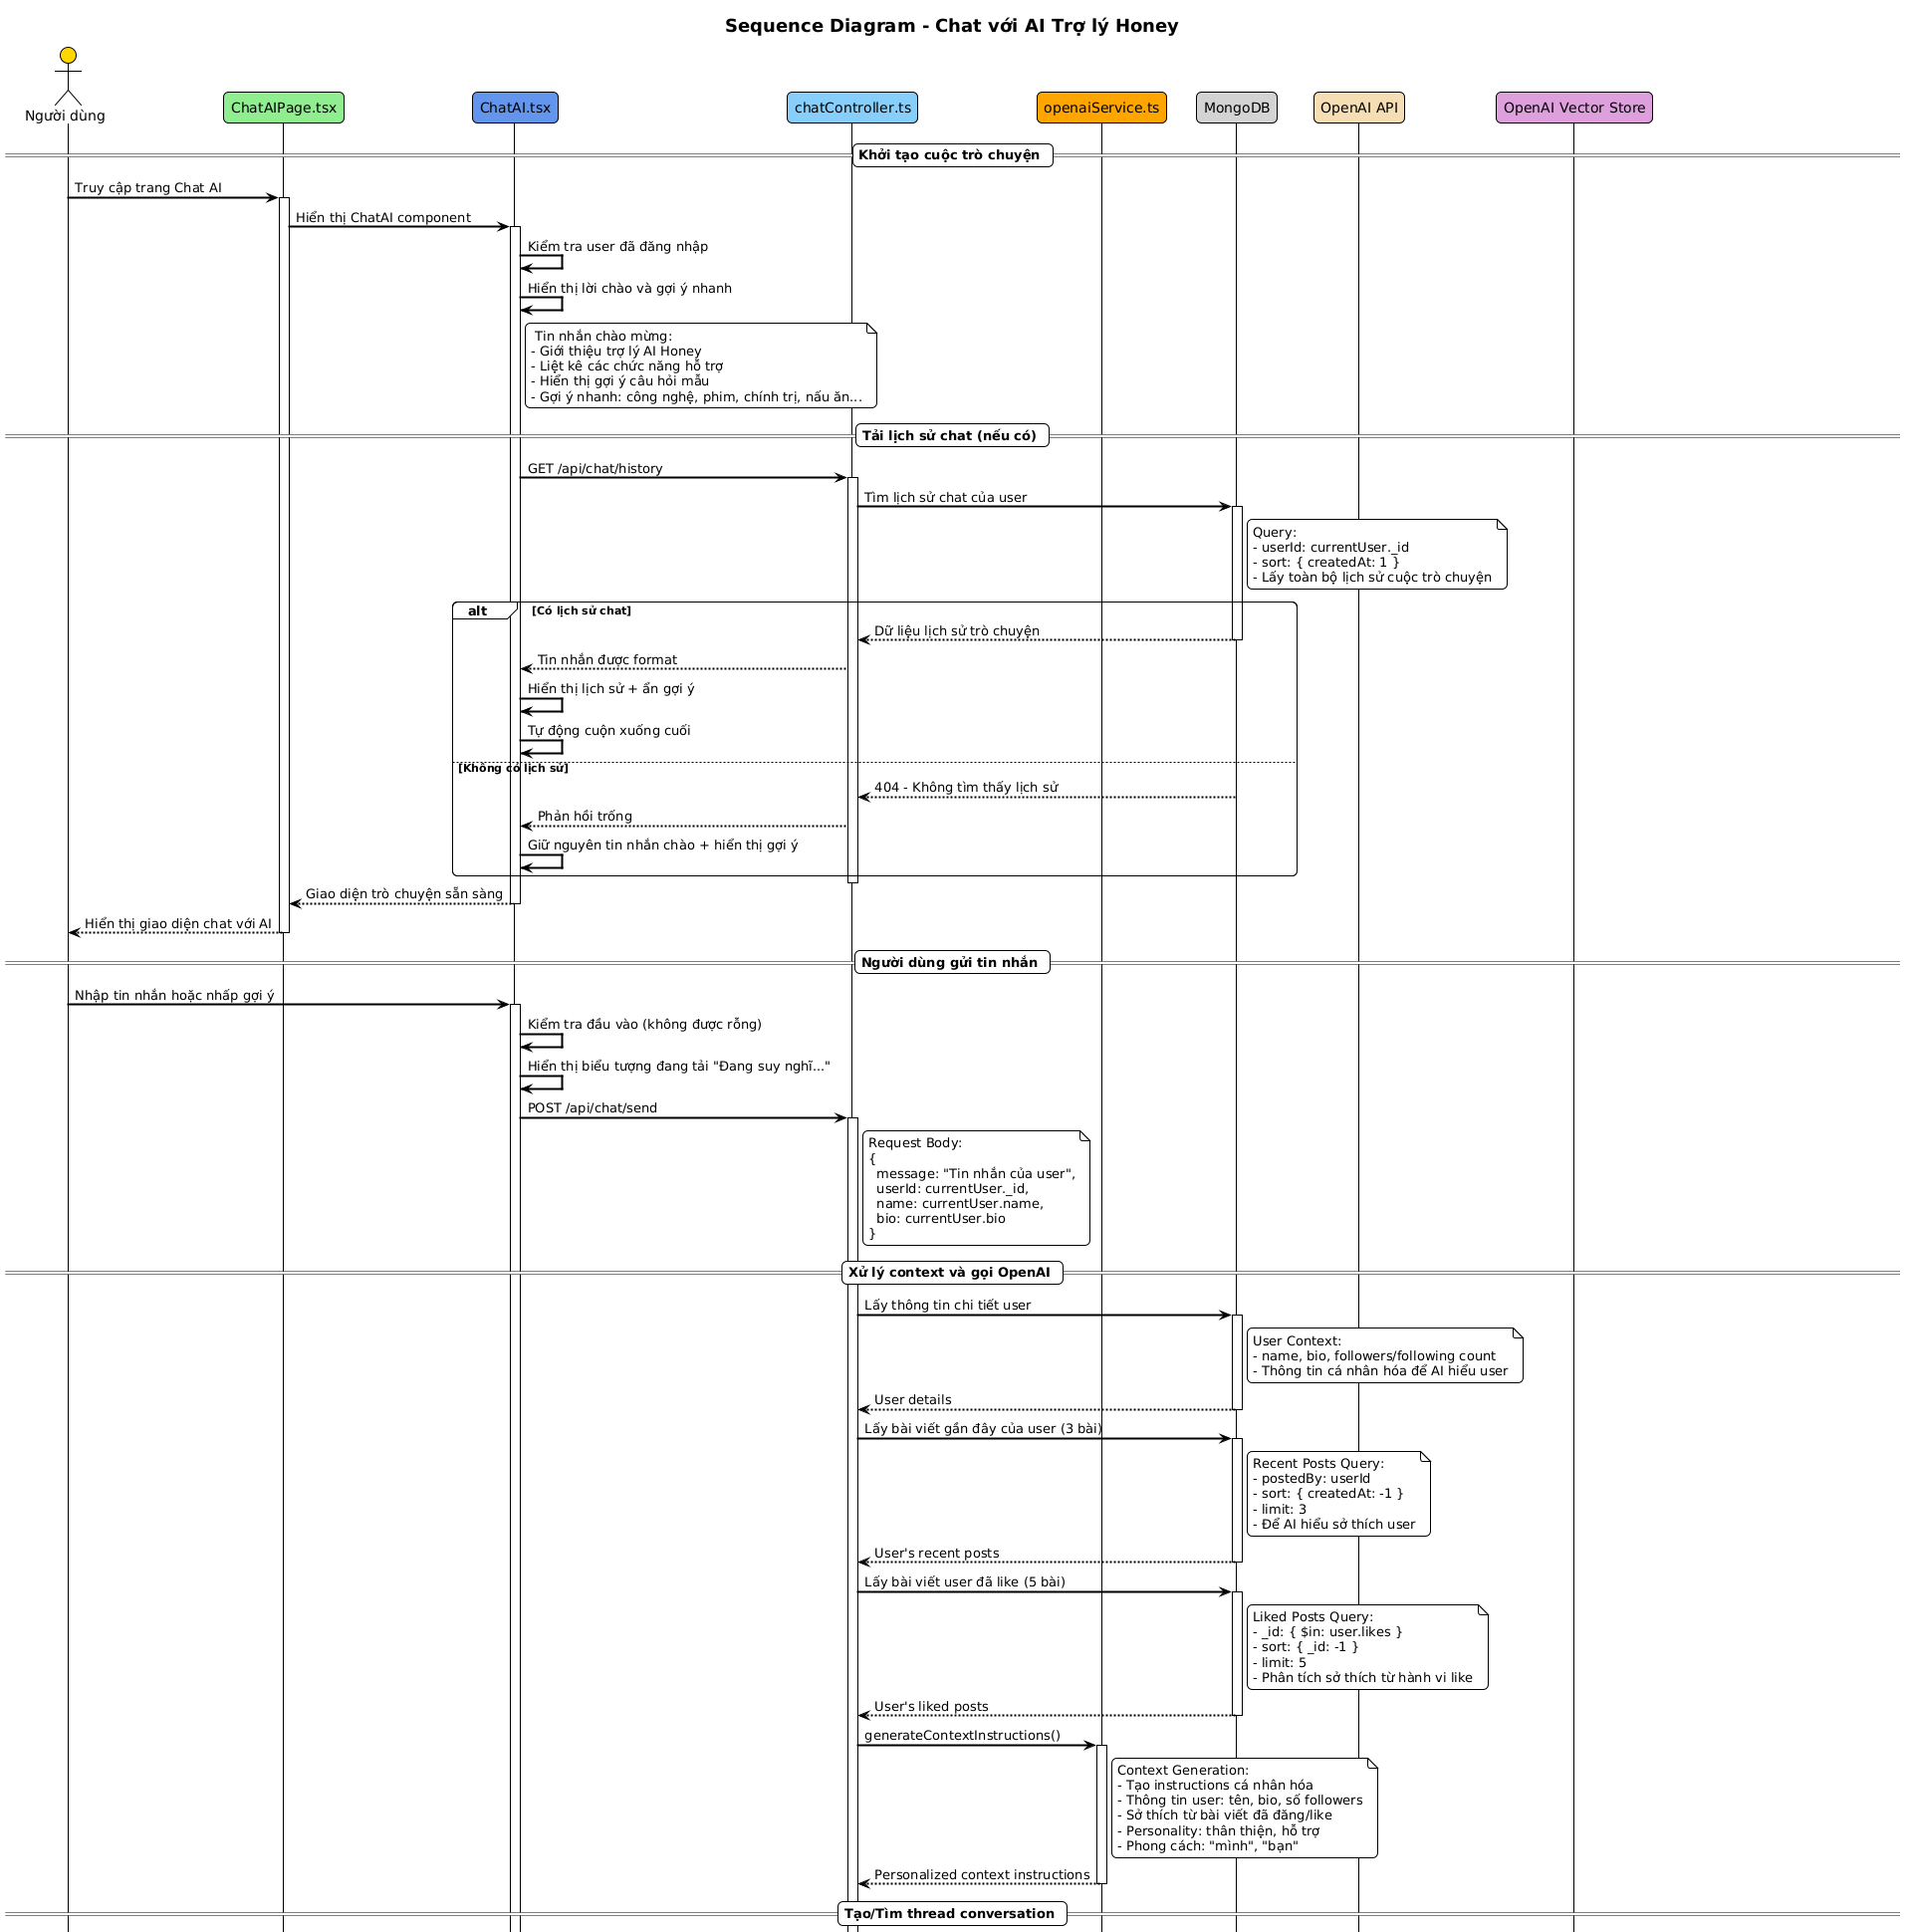
\includegraphics[width=1\textwidth]{image/sequence/chat-ai.png}
%     \caption{Hình ảnh Chat AI}
%     \label{fig:chat_ai}
% \end{figure}


% \begin{figure}[H]
%     \centering
%     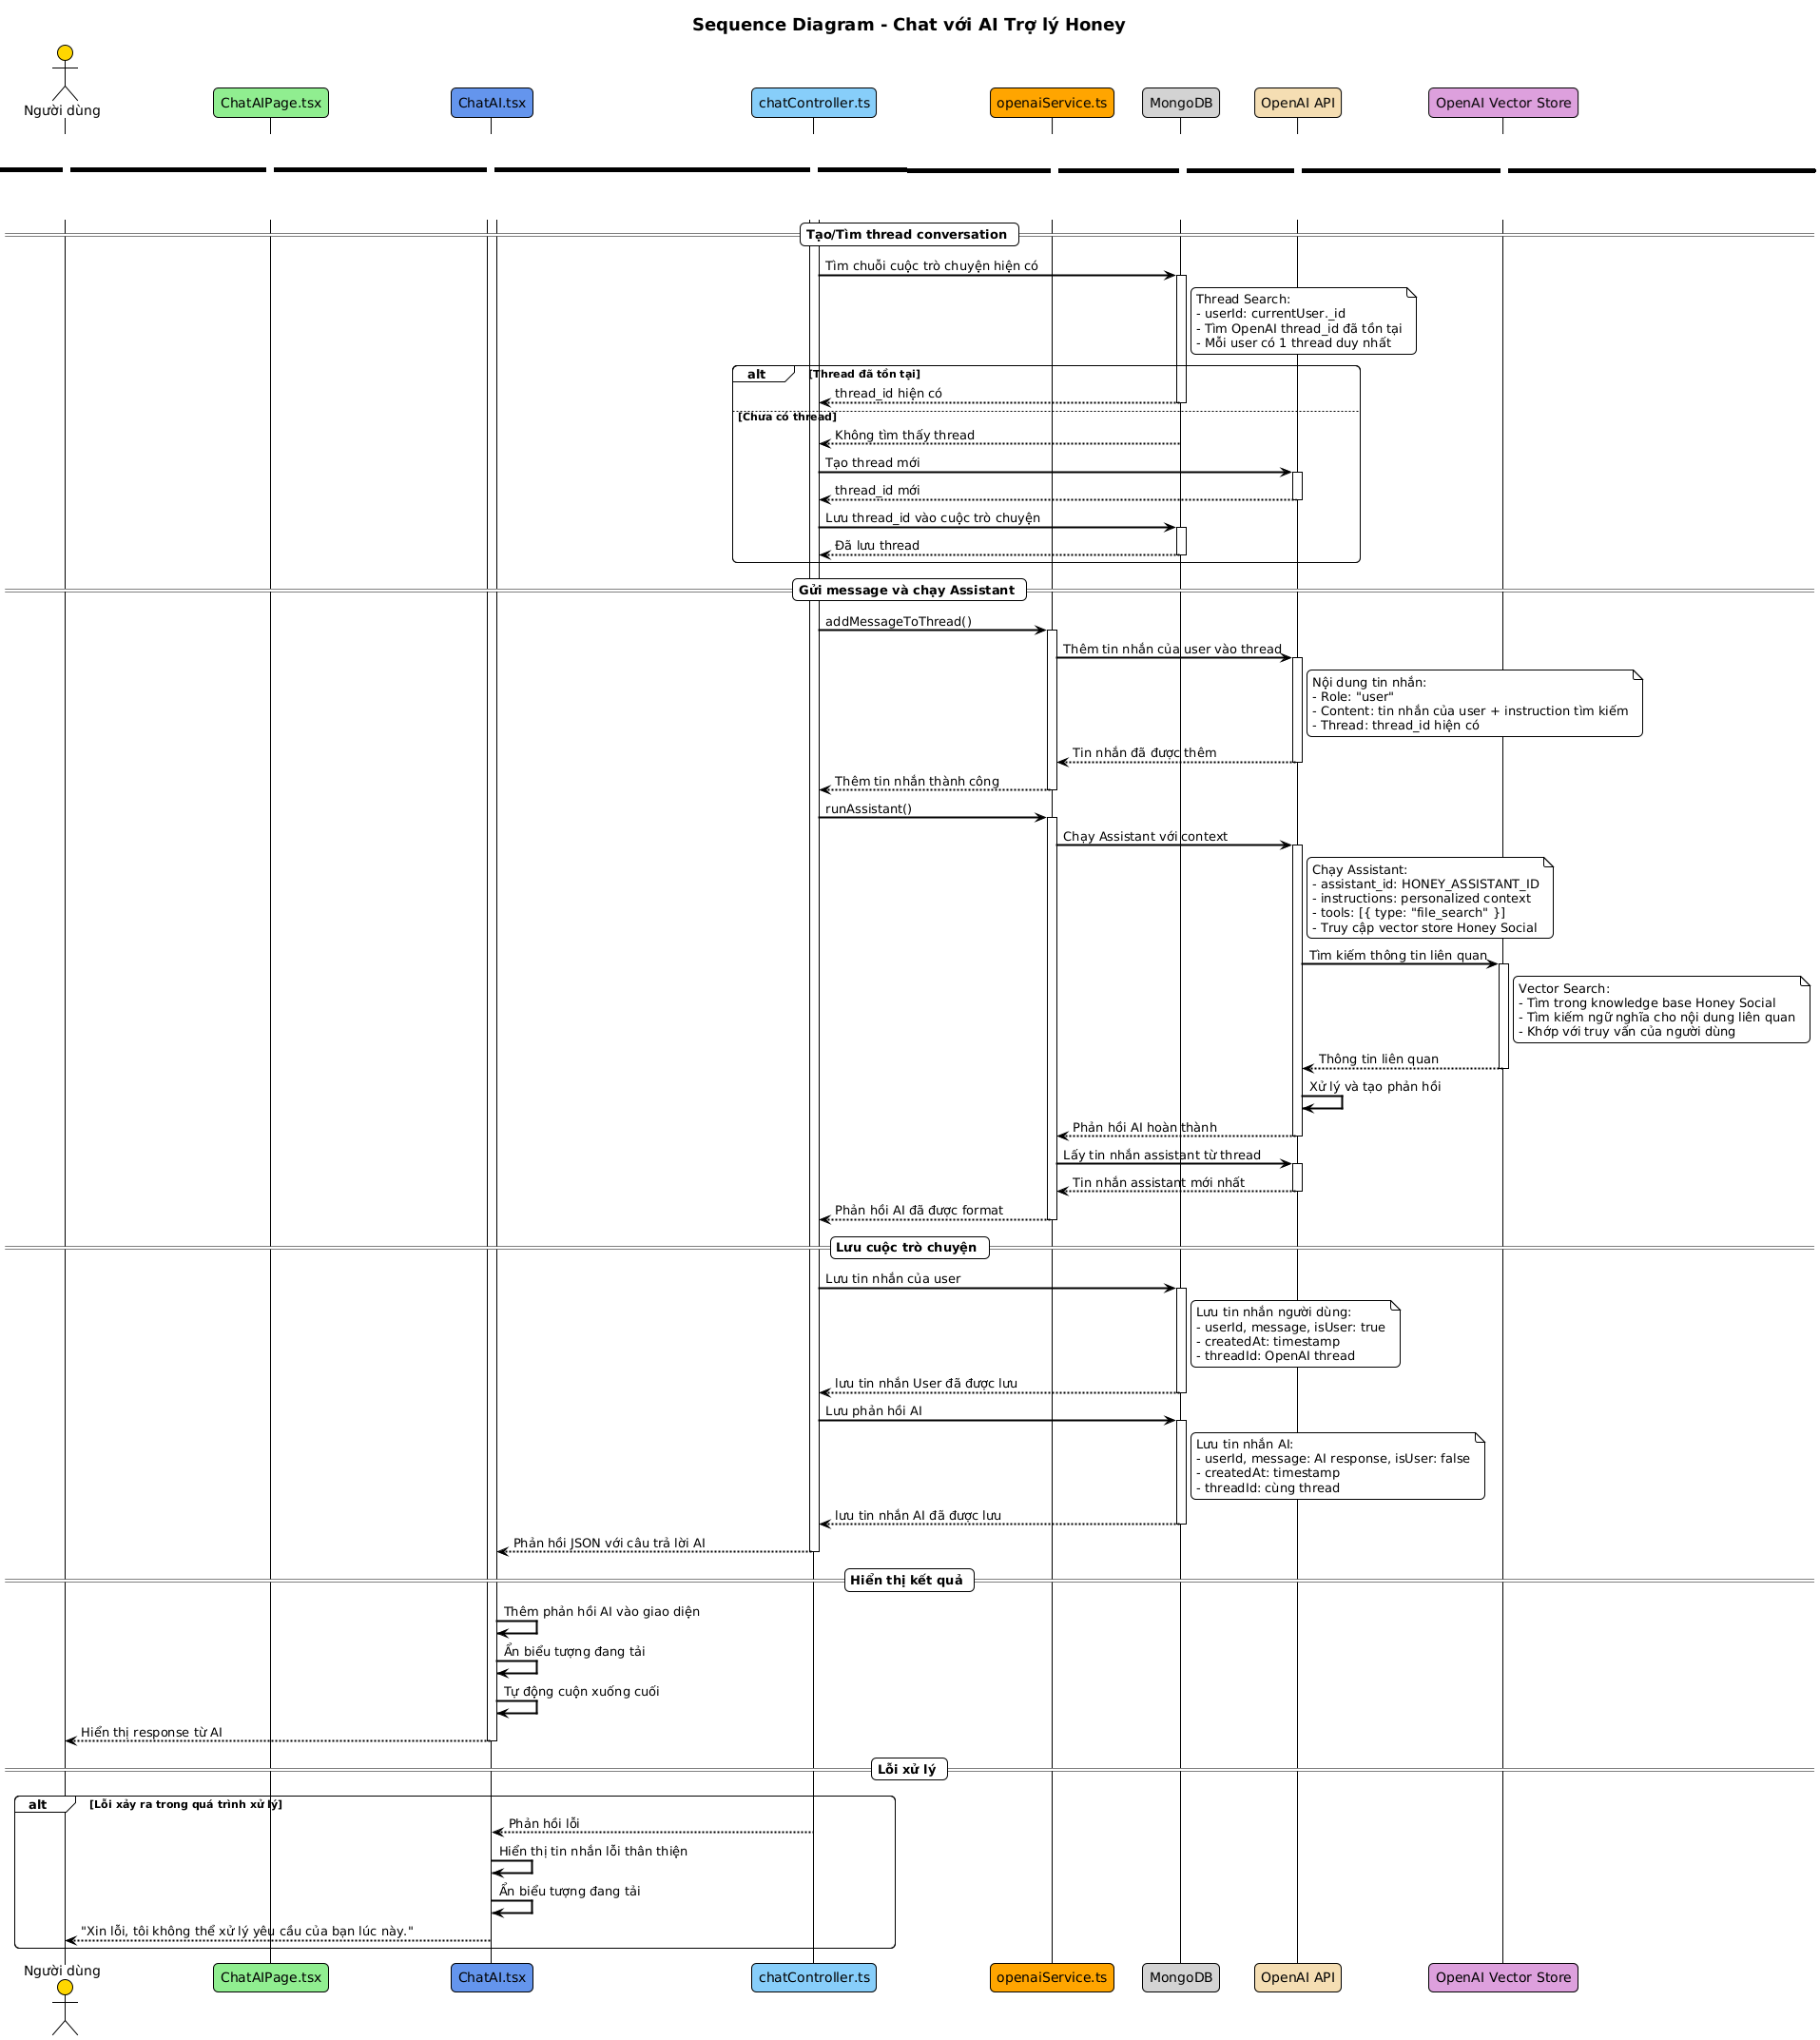
\includegraphics[width=1\textwidth]{image/sequence/chat-ai2.png}
%     \caption{Hình ảnh Chat AI 2}
%     \label{fig:chat_ai2}
% \end{figure}


% \begin{figure}[H]
%     \centering
%     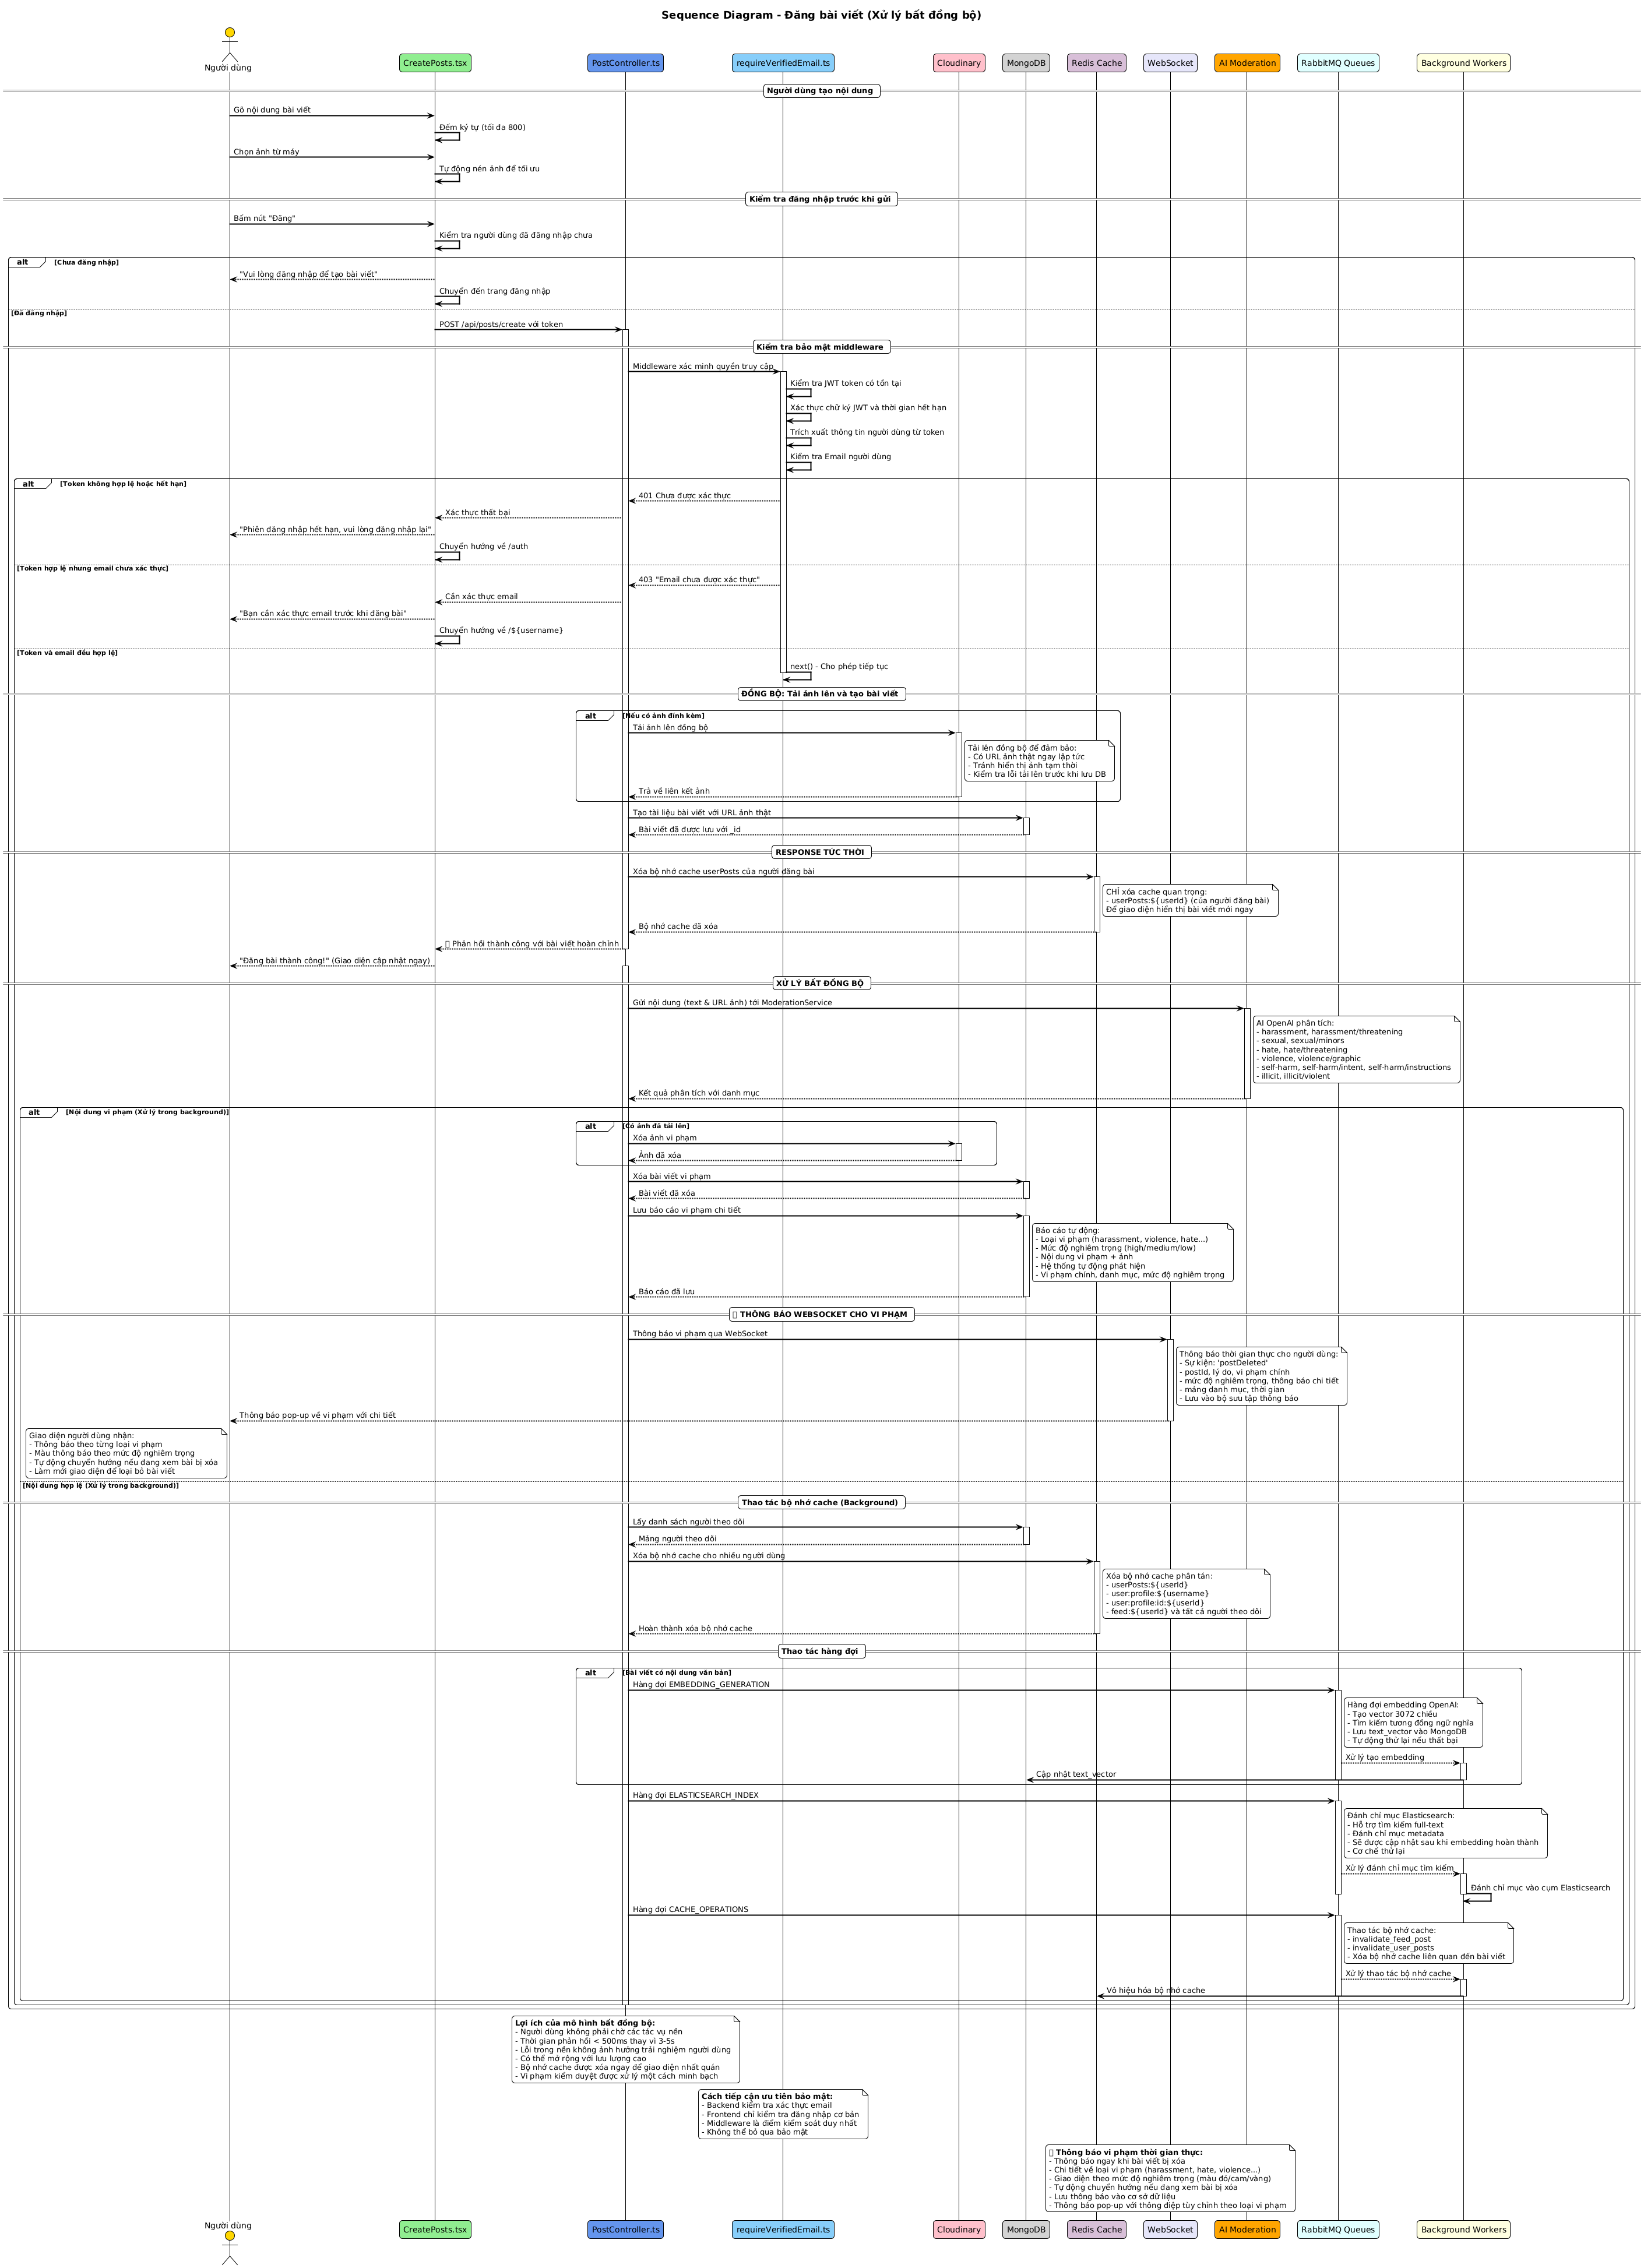
\includegraphics[width=1\textwidth]{image/sequence/dang-bai-viet.png}
%     \caption{Hình ảnh Đăng bài viết}
%     \label{fig:dang_bai_viet}
% \end{figure}

% \begin{figure}[H]
%     \centering
%     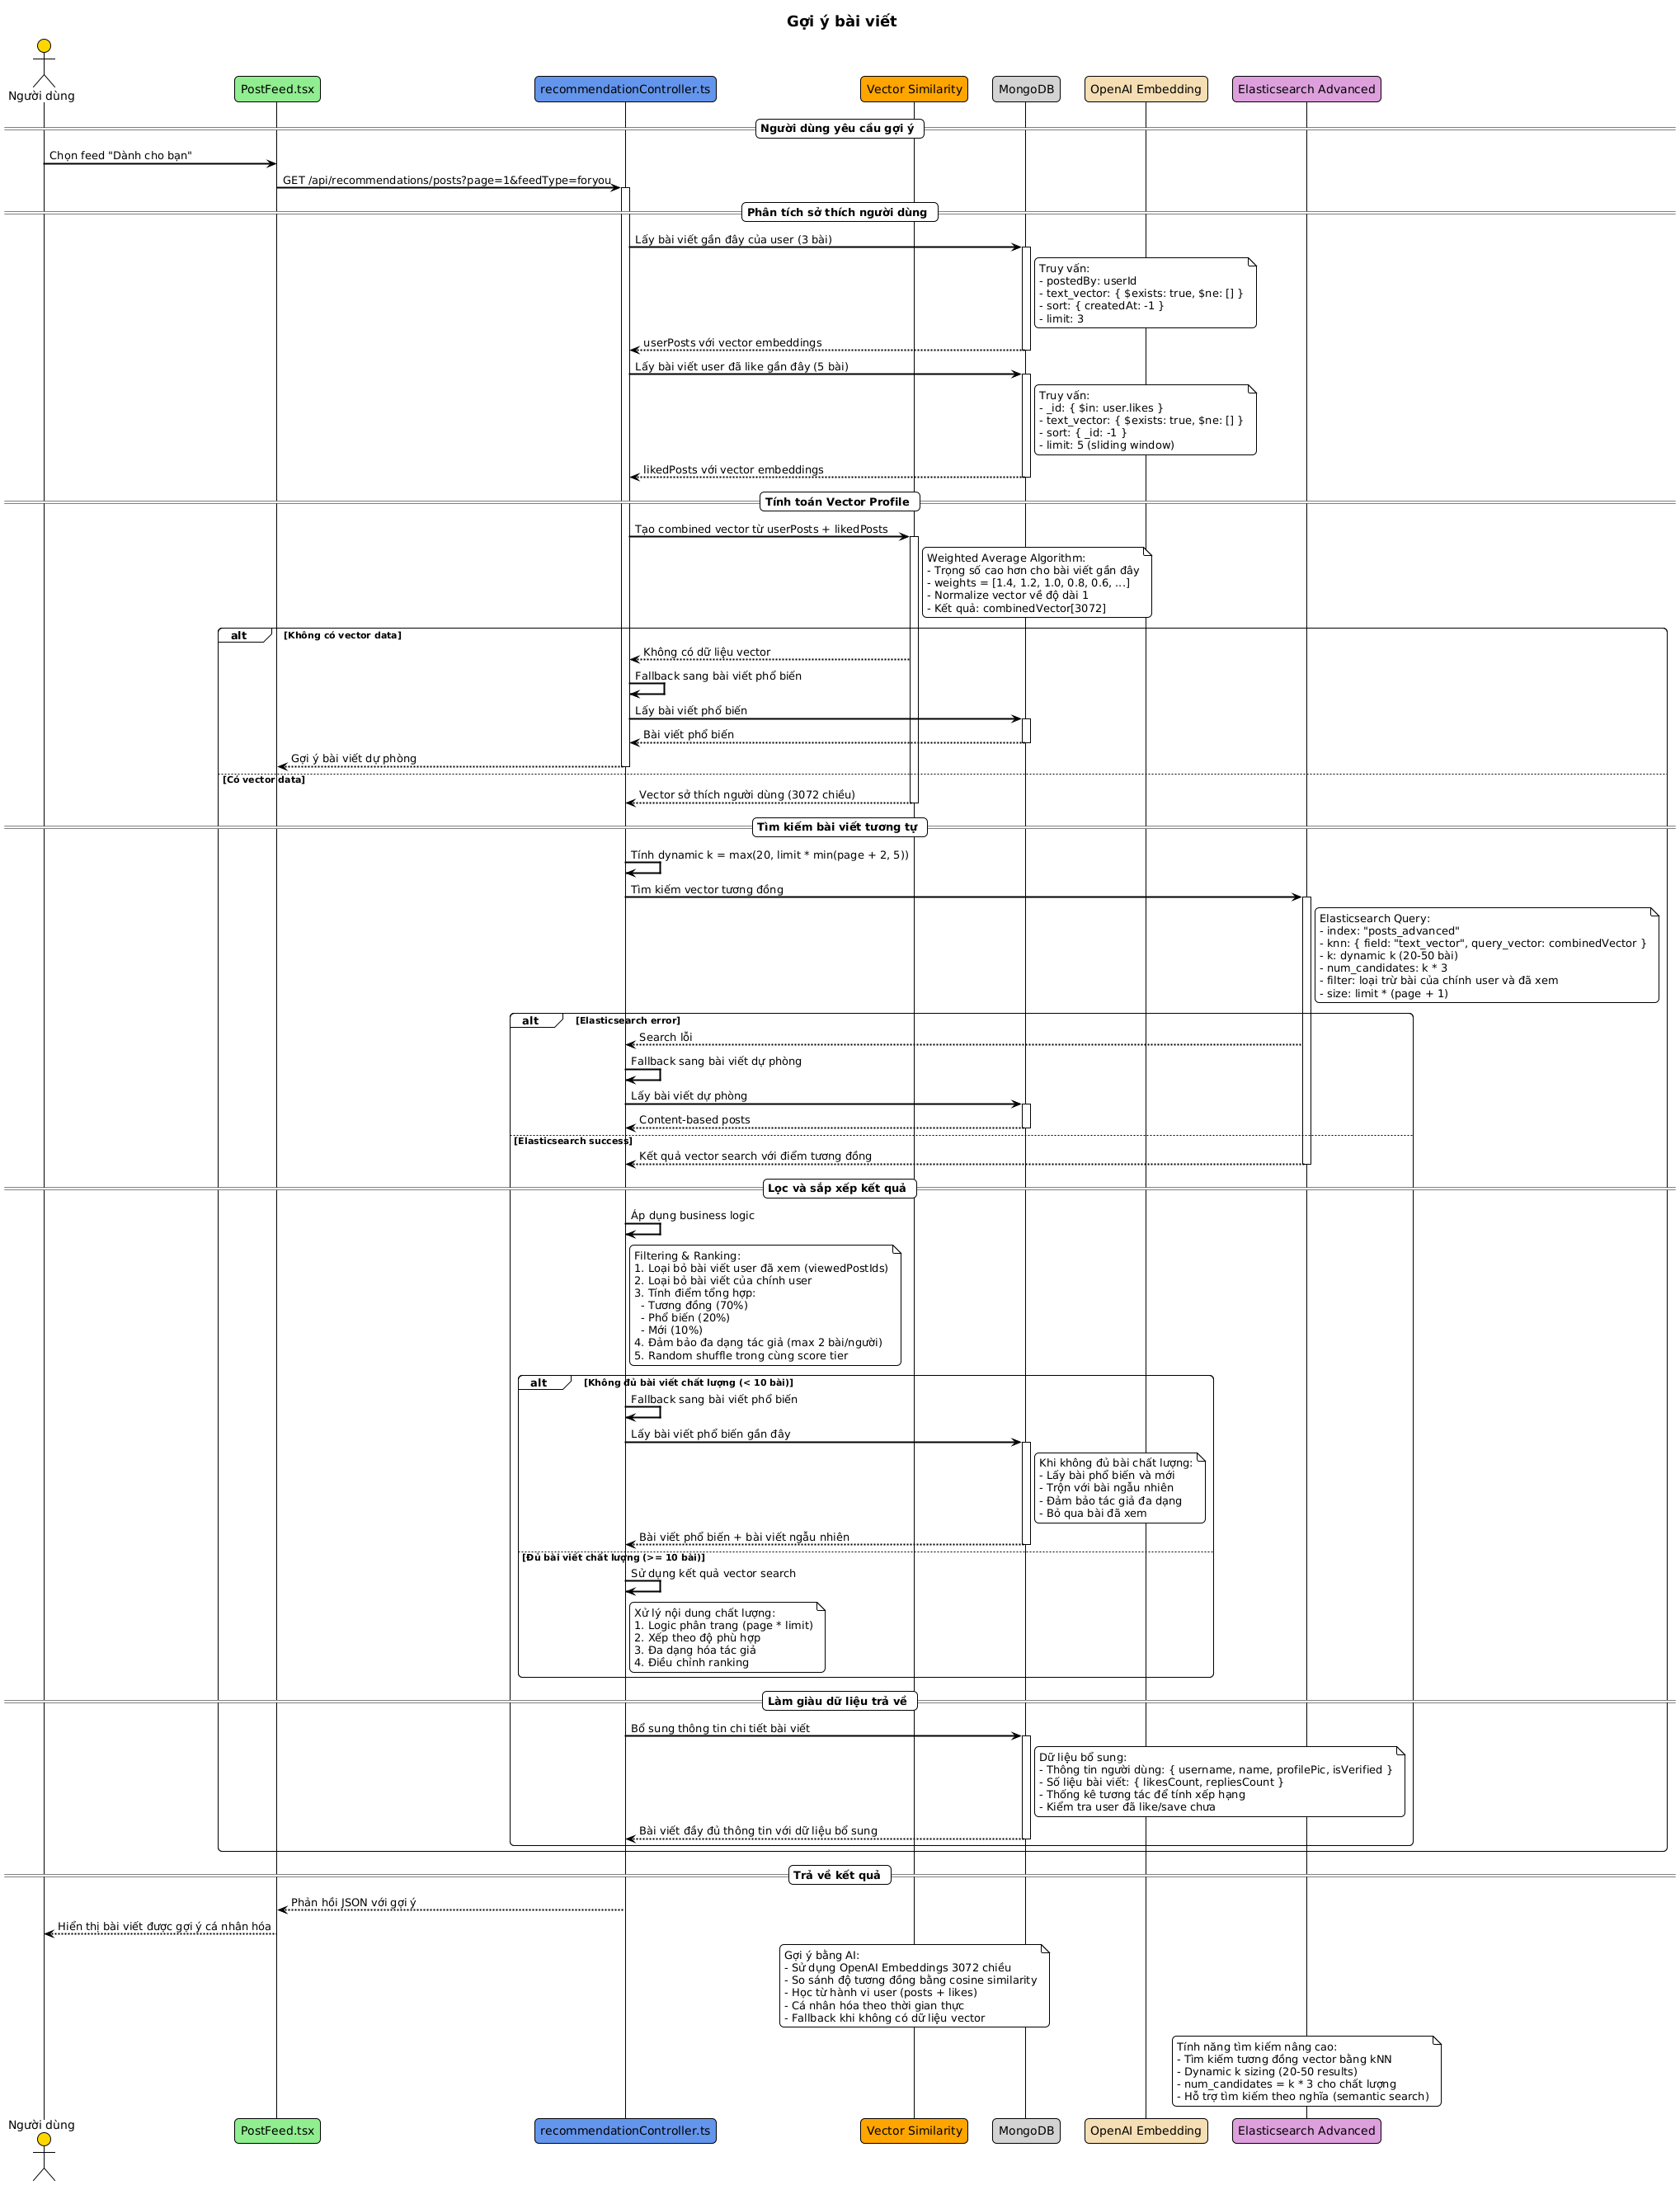
\includegraphics[width=1\textwidth]{image/sequence/goi-y-bai-viet.png}
%     \caption{Hình ảnh Gợi ý bài viết}
%     \label{fig:goi_y_bai_viet}
% \end{figure}

% \begin{figure}[H]
%     \centering
%     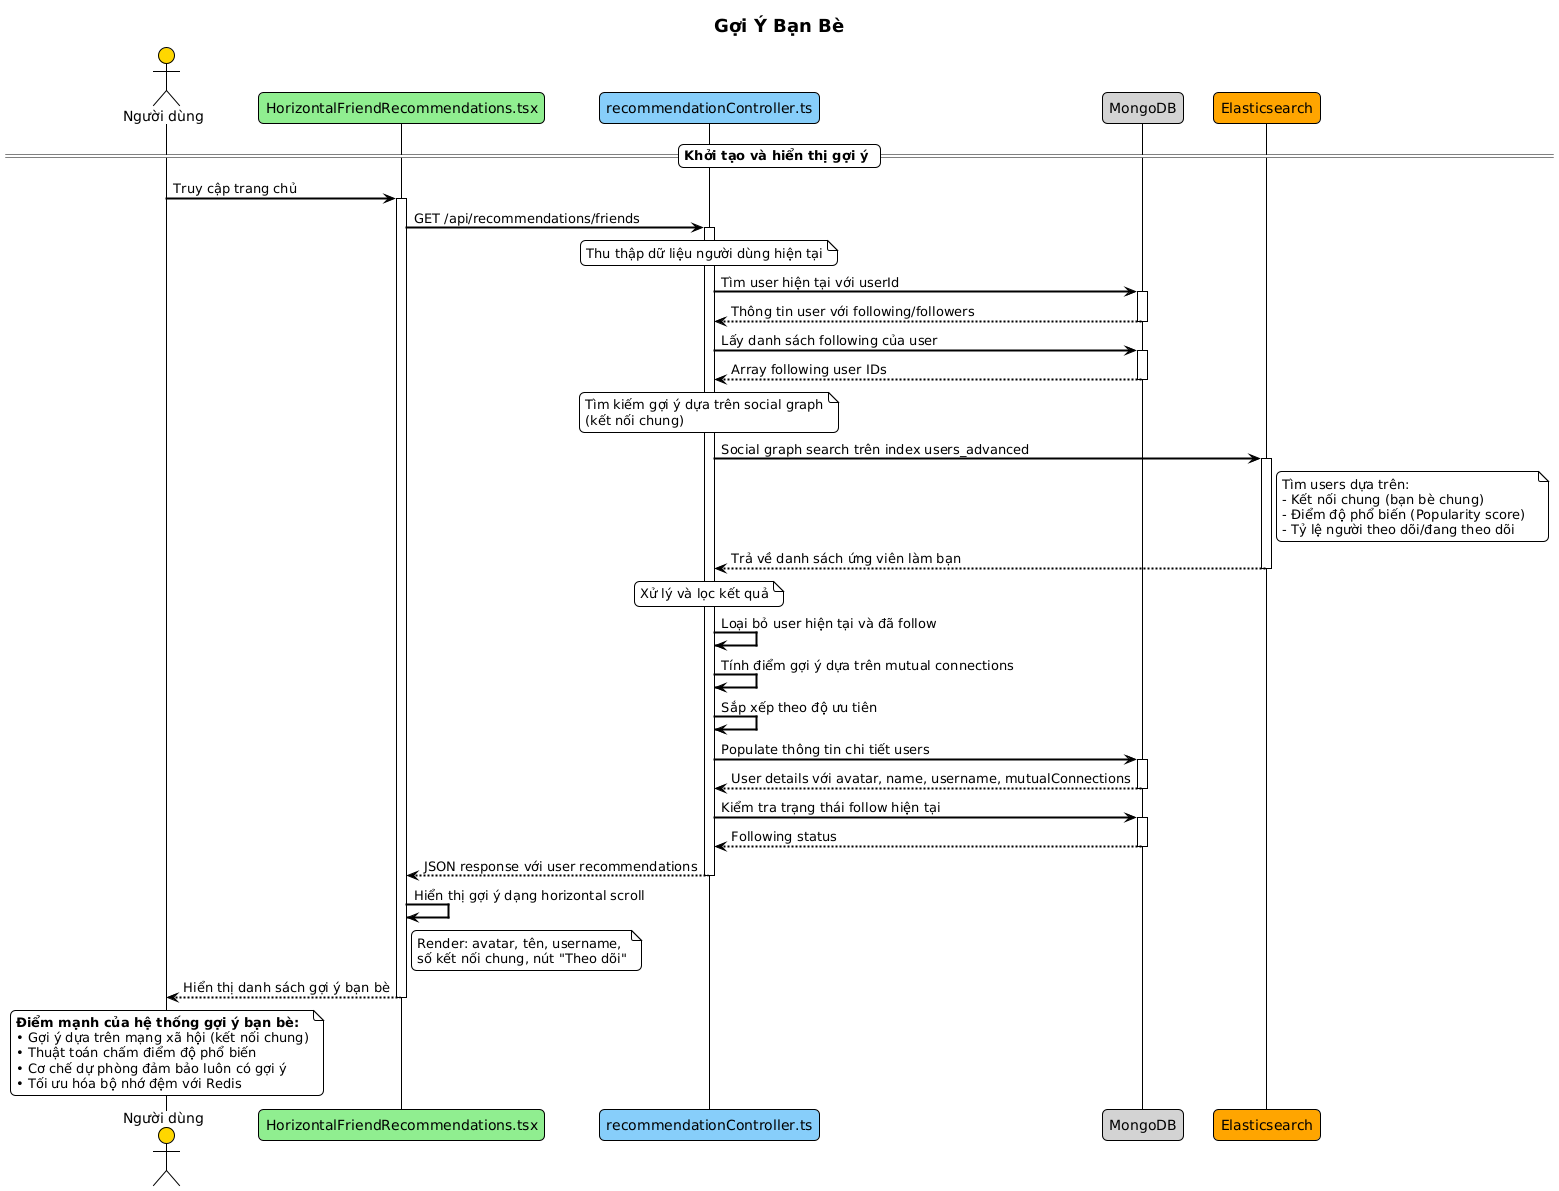
\includegraphics[width=1\textwidth]{image/sequence/goi-y-ban-be.png}
%     \caption{Hình ảnh Gợi ý bạn bè}
%     \label{fig:goi_y_ban_be}
% \end{figure}


% \begin{figure}[H]
%     \centering
%     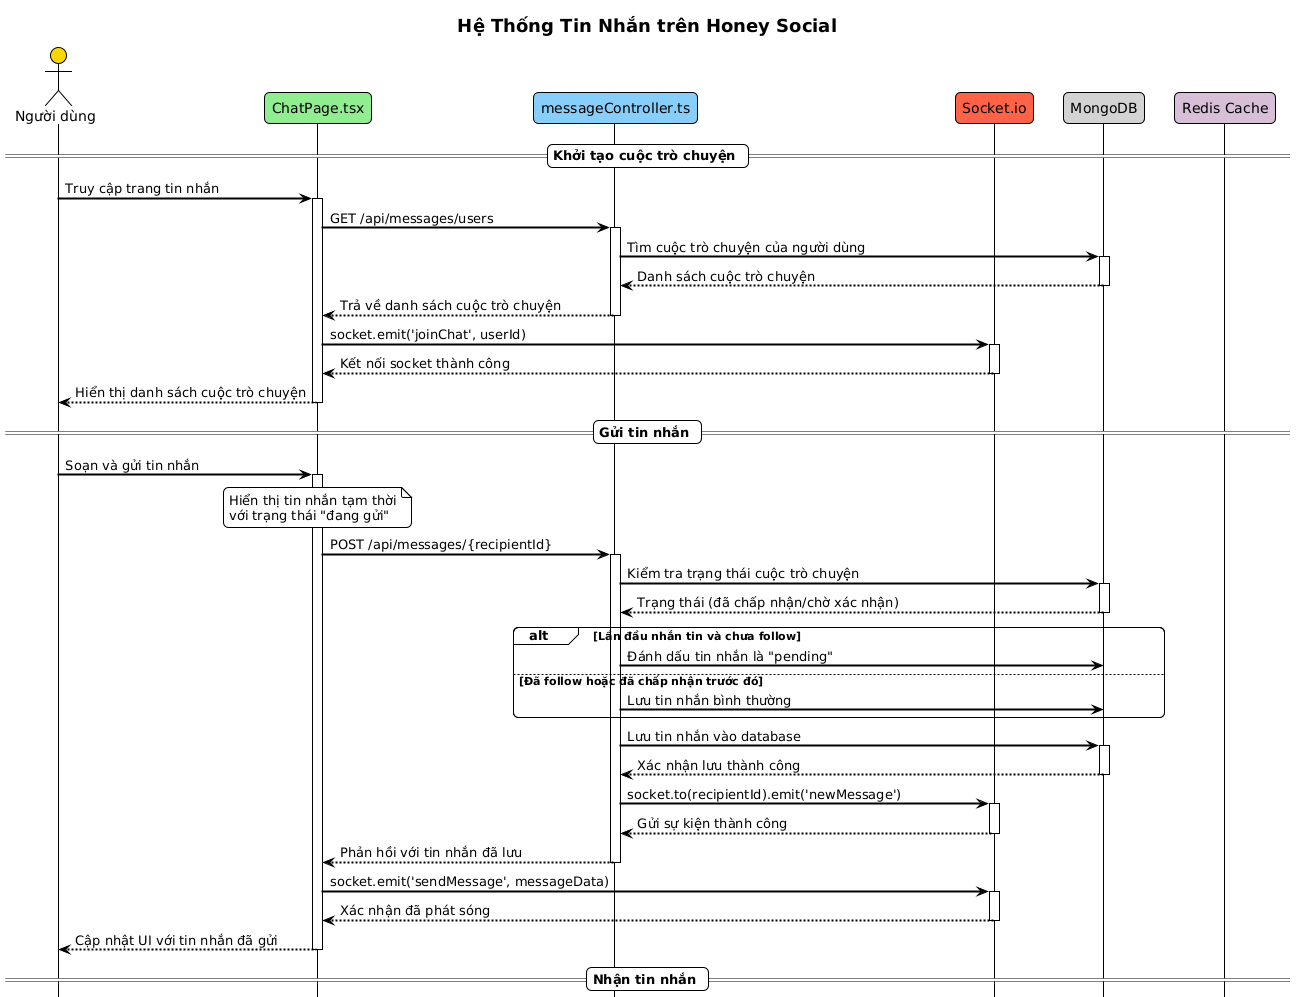
\includegraphics[width=1\textwidth]{image/sequence/message1.png}
%     \caption{Hình ảnh Hệ thống tin nhắn trên Honey Social}
%     \label{fig:message}
% \end{figure}


% \begin{figure}[H]
%     \centering
%     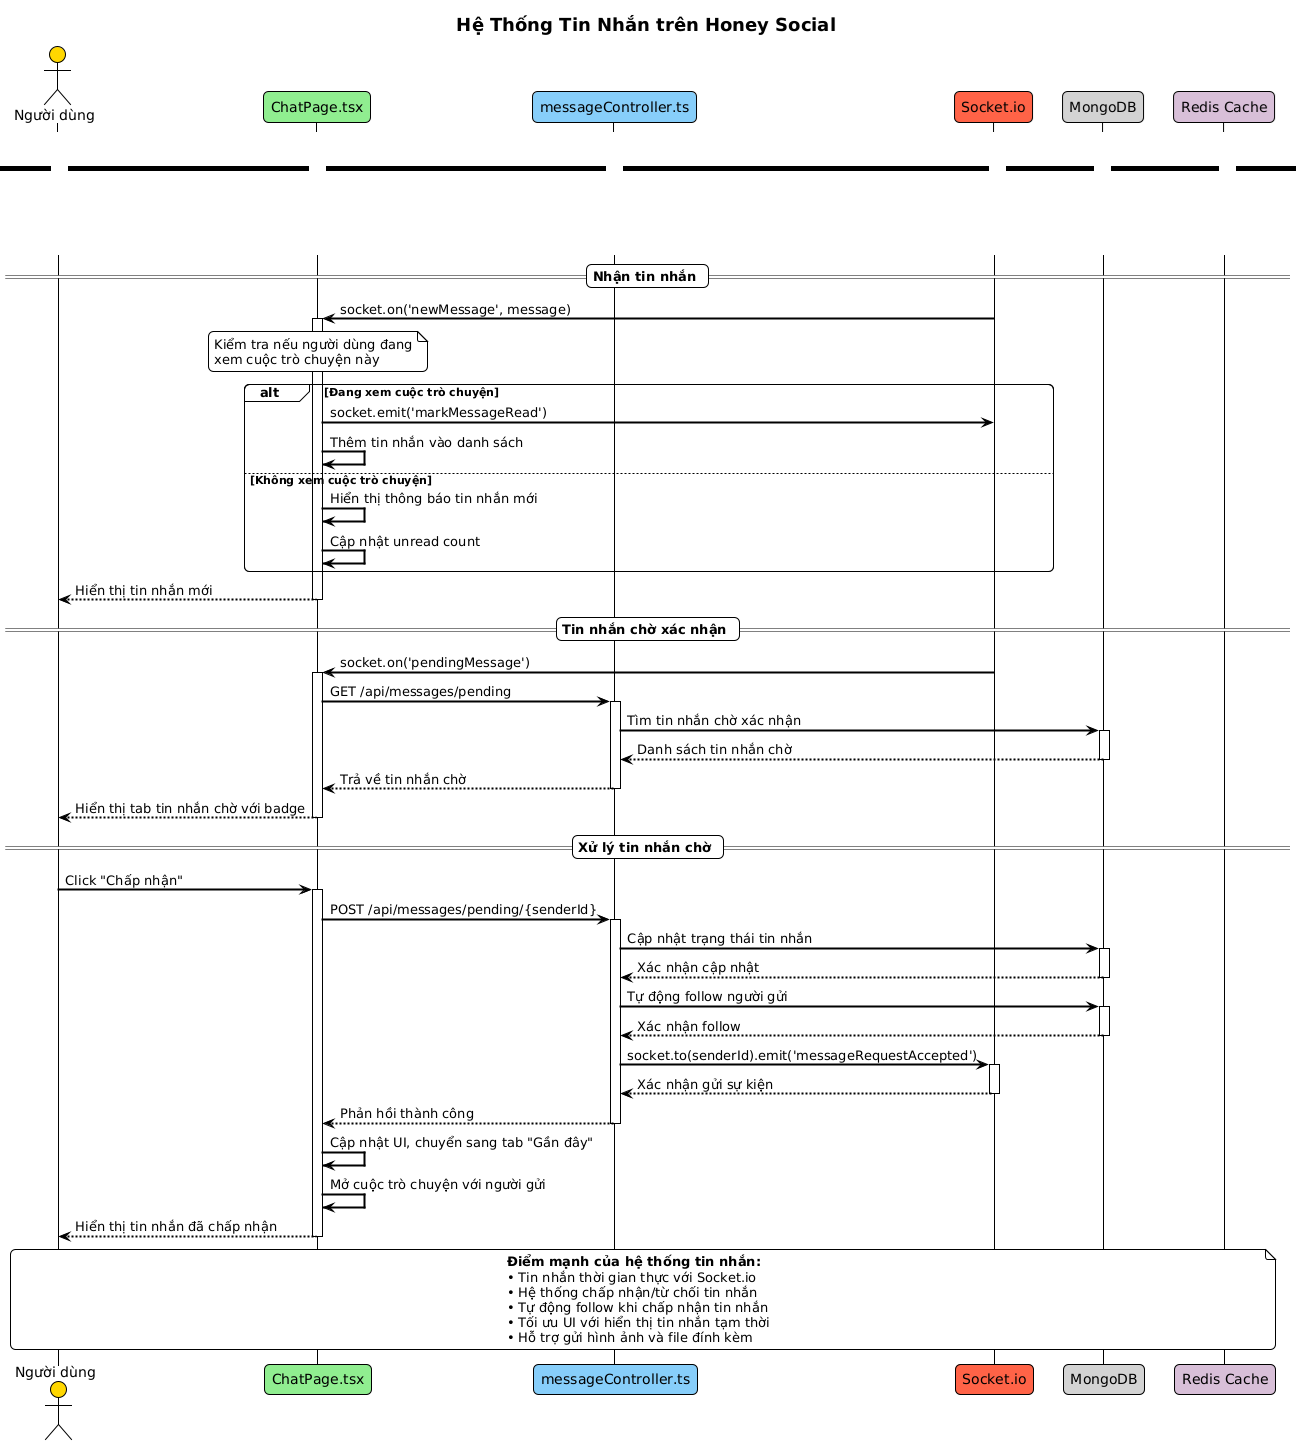
\includegraphics[width=1\textwidth]{image/sequence/message2.png}
%     \caption{Hình ảnh Hệ thống tin nhắn trên Honey Social 2}
%     \label{fig:message}
% \end{figure}




% \begin{figure}[H]
%     \centering
%     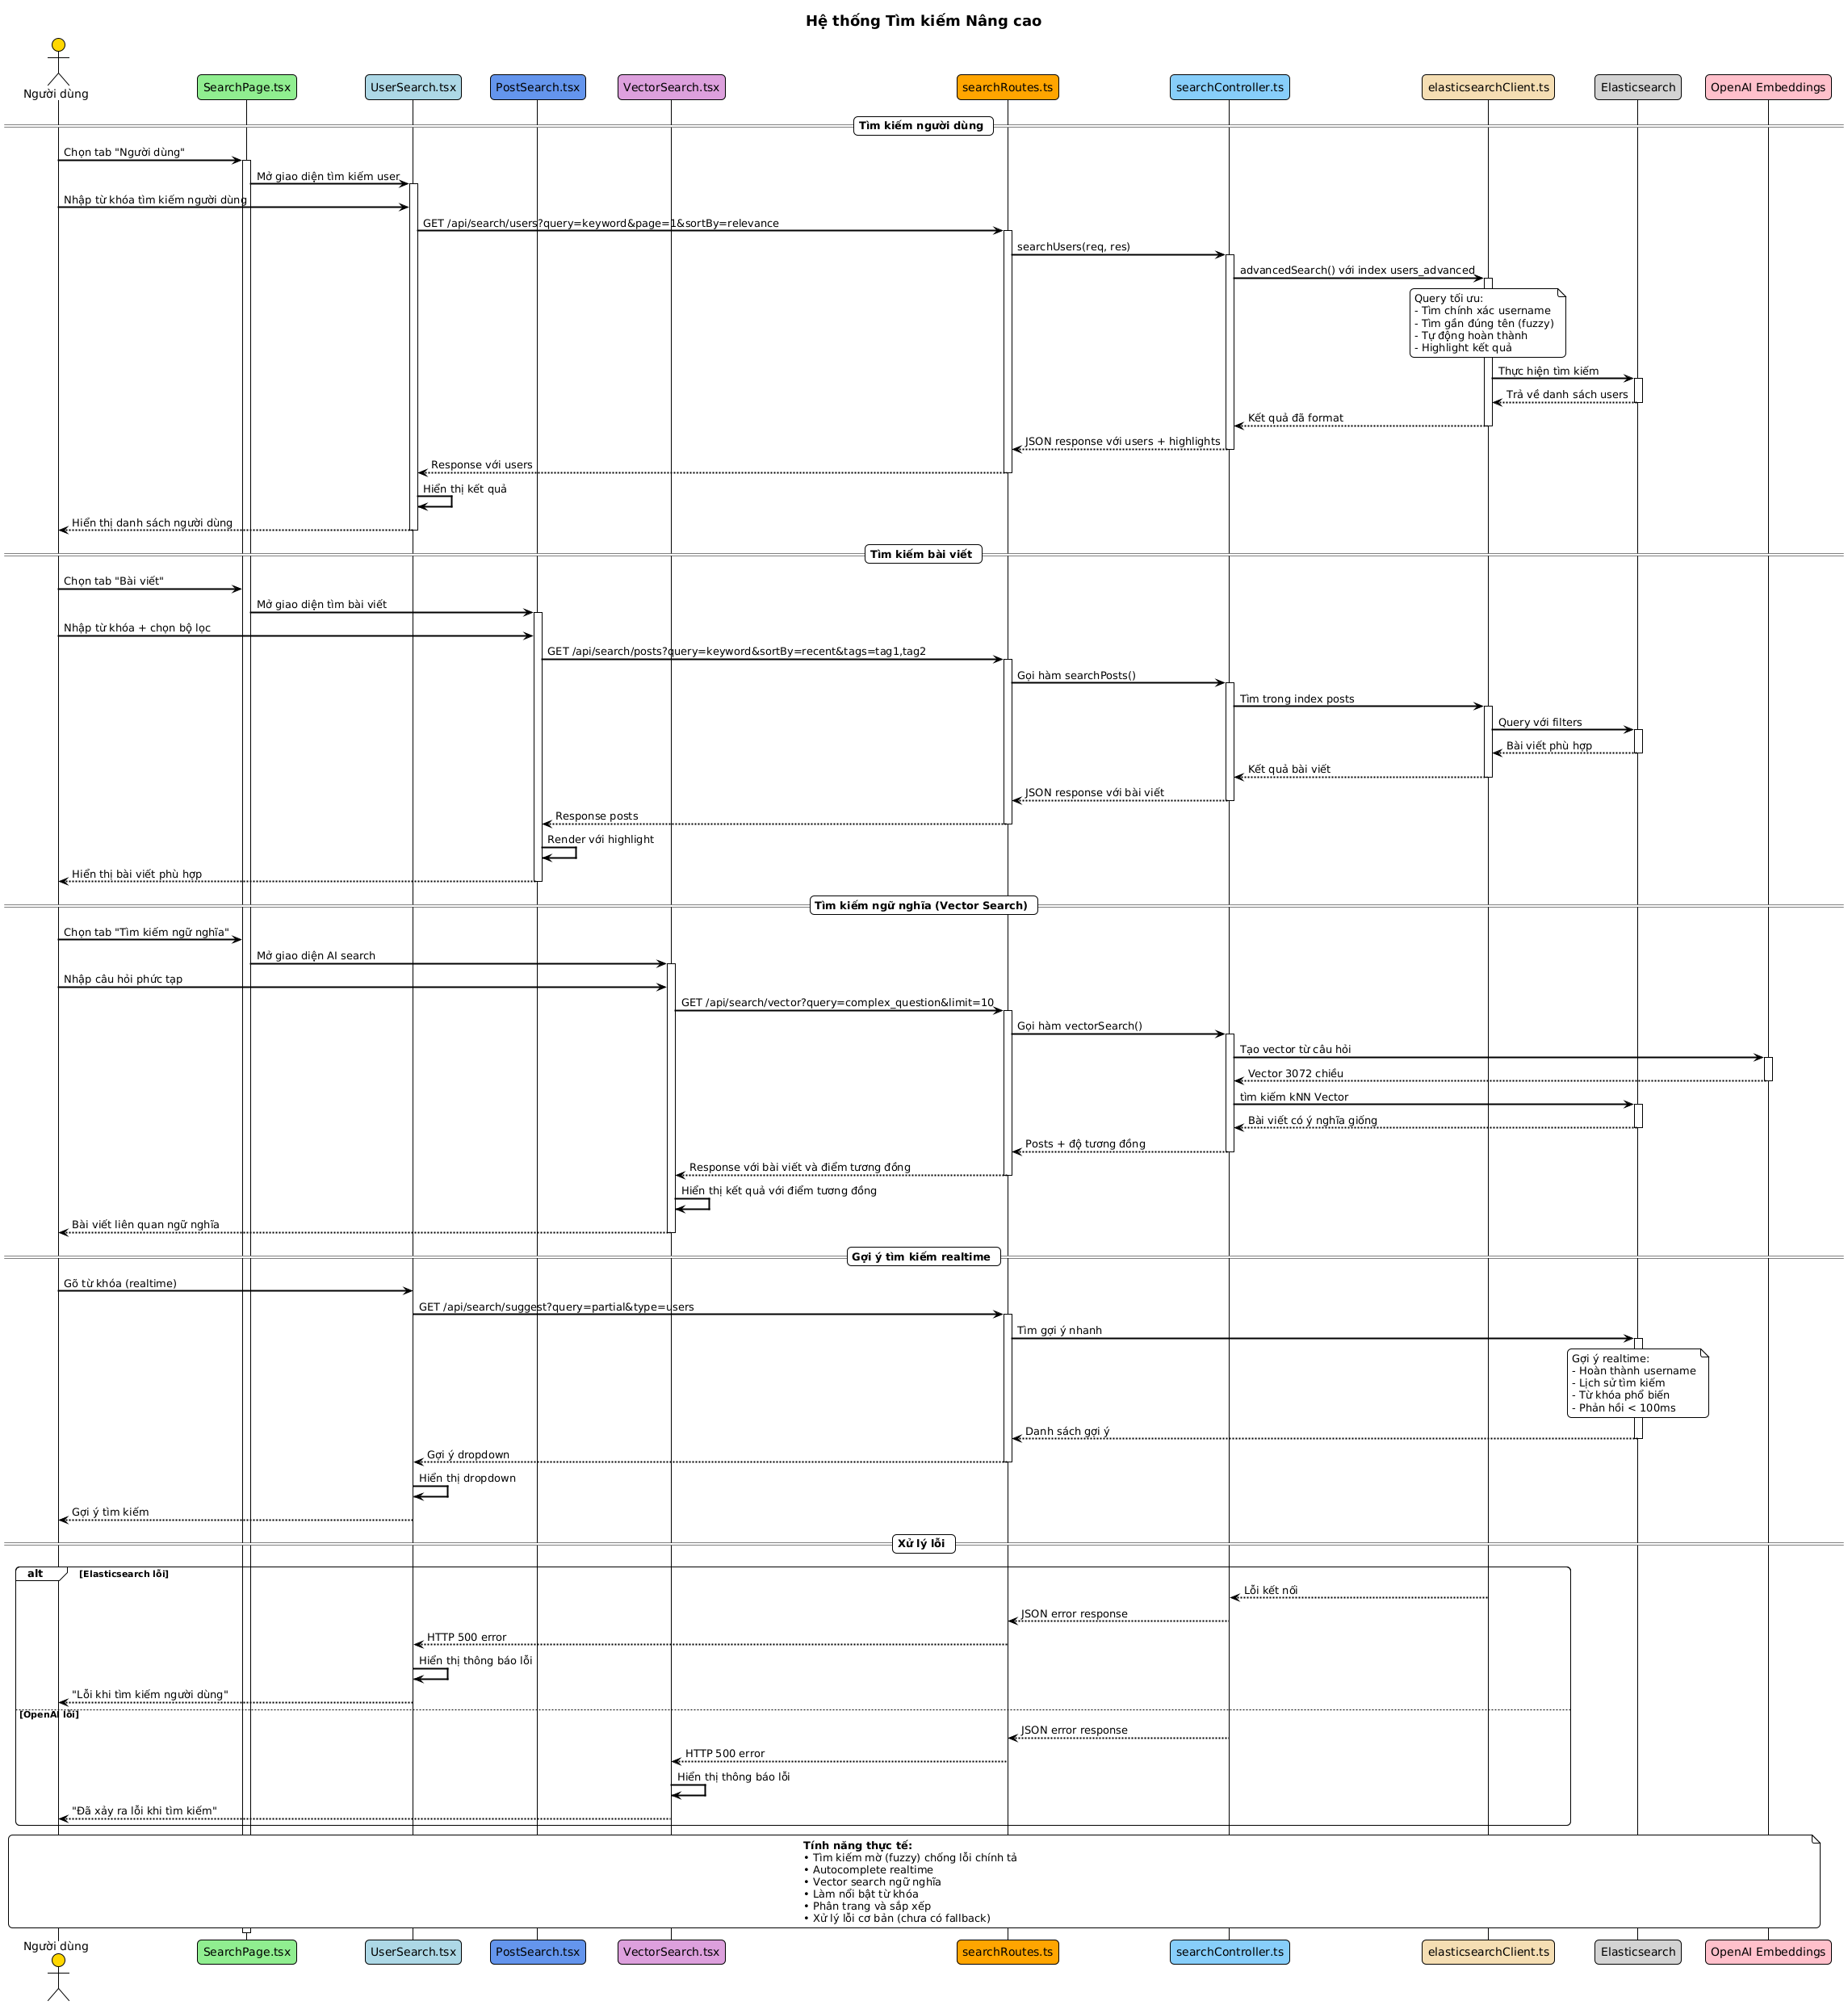
\includegraphics[width=1\textwidth]{image/sequence/tim-kiem-nang-cao.png}
%     \caption{Hình ảnh Tìm kiếm nâng cao}
%     \label{fig:tim_kiem_nang_cao}
% \end{figure}

% \newpage
% \section{\textbf{ CHƯƠNG 4: THIẾT KẾ CƠ SỞ DỮ LIỆU}}

% \textbf{1. posts}

% \begin{table}[H]
% \centering
% \renewcommand{\arraystretch}{1.3}
% \begin{tabular}{|p{4cm}|p{4cm}|p{2cm}|p{2cm}|p{2cm}|}
% \hline
% \textbf{Name} & \textbf{Data Type} & \textbf{Array} & \textbf{Key} & \textbf{Required} \\
% \hline
% \_id         & objectId &  & Yes & Yes \\
% postedBy     & objectId &  &     & Yes \\
% text         & string   &  &     & Yes \\
% text\_vector & double   & Yes &     & Yes \\
% img          & string   &  &     & Yes \\
% likes        & objectId & Yes &     & Yes \\
% likesCount   & double   &  &     & Yes \\
% replies      & string   & Yes &     & Yes \\
% createdAt    & date     &  &     & Yes \\
% updatedAt    & date     &  &     & Yes \\
% \hline
% \end{tabular}
% \caption{Cấu trúc của bảng \texttt{posts}}
% \end{table}


% \textbf{2. chatmessages}

% \begin{table}[H]
% \centering
% \renewcommand{\arraystretch}{1.3}
% \begin{tabular}{|p{4cm}|p{4cm}|p{2cm}|p{2cm}|p{2cm}|}
% \hline
% \textbf{Name} & \textbf{Data Type} & \textbf{Array} & \textbf{Key} & \textbf{Required} \\
% \hline
% \_id         & objectId &  & Yes & Yes \\
% userId       & objectId &  &     & Yes \\
% isUser       & bool     &  &     & Yes \\
% message      & string   &  &     & Yes \\
% createdAt    & date     &  &     & Yes \\
% updatedAt    & date     &  &     & Yes \\
% \hline
% \end{tabular}
% \caption{Cấu trúc của bảng \texttt{chatmessages}}
% \end{table}

% \newpage
% \textbf{3. threads}


% \begin{table}[H]
% \centering
% \renewcommand{\arraystretch}{1.3}
% \begin{tabular}{|p{4cm}|p{4cm}|p{2cm}|p{2cm}|p{2cm}|}
% \hline
% \textbf{Name} & \textbf{Data Type} & \textbf{Array} & \textbf{Key} & \textbf{Required} \\
% \hline
% \_id         & objectId &  & Yes & Yes \\
% userId       & objectId &  &     & Yes \\
% createdAt    & date     &  &     & Yes \\
% lastUsed     & date     &  &     & Yes \\
% threadId     & string   &  &     & Yes \\
% \hline
% \end{tabular}
% \caption{Cấu trúc của bảng \texttt{threads}}
% \end{table}

% \newpage
% \textbf{4. reports}

% \begin{table}[H]
% \centering
% \renewcommand{\arraystretch}{1.3}
% \begin{tabular}{|p{4cm}|p{4cm}|p{2cm}|p{2cm}|p{2cm}|}
% \hline
% \textbf{Name} & \textbf{Data Type} & \textbf{Array} & \textbf{Key} & \textbf{Required} \\
% \hline
% \_id               & objectId &  & Yes & Yes \\
% reportedBy         & any      &  &     & Yes \\
% reportedContent    & objectId &  &     & Yes \\
% contentType        & string   &  &     & Yes \\
% reason             & string   &  &     & Yes \\
% details            & string   &  &     & Yes \\
% status             & string   &  &     & Yes \\
% createdAt          & date     &  &     & Yes \\
% updatedAt          & date     &  &     & Yes \\
% resolvedBy         & objectId &  &     & Yes \\
% postId             & objectId &  &     & Yes \\
% postContent        & string   &  &     & Yes \\
% moderationResult   & string   &  &     & Yes \\
% resolution         & string   &  &     & Yes \\
% severity           & string   &  &     & Yes \\
% reportedByUsername & string   &  &     & Yes \\
% postImage          & any      &  &     & Yes \\
% \hline
% \end{tabular}
% \caption{Cấu trúc của bảng \texttt{reports}}
% \end{table}


% \newpage
% \textbf{5. verifications}

% \begin{table}[H]
% \centering
% \renewcommand{\arraystretch}{1.3}
% \begin{tabular}{|p{4cm}|p{4cm}|p{2cm}|p{2cm}|p{2cm}|}
% \hline
% \textbf{Name} & \textbf{Data Type} & \textbf{Array} & \textbf{Key} & \textbf{Required} \\
% \hline
% \_id         & objectId &  & Yes & Yes \\
% userId       & objectId &  &     & Yes \\
% email        & string   &  &     & Yes \\
% code         & string   &  &     & Yes \\
% createdAt    & date     &  &     & Yes \\
% \hline
% \end{tabular}
% \caption{Cấu trúc của bảng \texttt{verifications}}
% \end{table}

% \newpage
% \textbf{6. messages}

% \begin{table}[H]
% \centering
% \renewcommand{\arraystretch}{1.3}
% \begin{tabular}{|p{4cm}|p{4cm}|p{2cm}|p{2cm}|p{2cm}|}
% \hline
% \textbf{Name} & \textbf{Data Type} & \textbf{Array} & \textbf{Key} & \textbf{Required} \\
% \hline
% \_id          & objectId &  & Yes & Yes \\
% sender        & objectId &  &     & Yes \\
% recipient     & objectId &  &     & Yes \\
% messageType   & string   &  &     & Yes \\
% text          & string   &  &     & Yes \\
% media         & null     &  &     &     \\
% file          & string   &  &     &     \\
% fileName      & null     &  &     &     \\
% fileSize      & null     &  &     &     \\
% fileType      & null     &  &     &     \\
% thumbnailUrl  & null     &  &     &     \\
% duration      & null     &  &     &     \\
% read          & bool     &  &     & Yes \\
% createdAt     & date     &  &     & Yes \\
% updatedAt     & date     &  &     & Yes \\
% cloudinary    & string   &  &     & Yes \\
% fileInfo      & string   &  &     & Yes \\
% mediaDetails  & string   &  &     & Yes \\
% status        & string   &  &     & Yes \\
% img           & string   &  &     & Yes \\
% pending       & bool     &  &     & Yes \\
% \hline
% \end{tabular}
% \caption{Cấu trúc của bảng \texttt{messages}}
% \end{table}
% \newpage
% \textbf{7. users}

% \begin{table}[H]
% \centering
% \renewcommand{\arraystretch}{1.3}
% \begin{tabular}{|p{4cm}|p{4cm}|p{2cm}|p{2cm}|p{2cm}|}
% \hline
% \textbf{Name} & \textbf{Data Type} & \textbf{Array} & \textbf{Key} & \textbf{Required} \\
% \hline
% \_id             & objectId &     & Yes & Yes \\
% name            & string   &     &     & Yes \\
% username        & string   &     &     & Yes \\
% email           & string   &     &     & Yes \\
% password        & string   &     &     & Yes \\
% profilePic      & string   &     &     & Yes \\
% followers       & string   & Yes &     & Yes \\
% following       & string   & Yes &     & Yes \\
% bio             & string   &     &     & Yes \\
% isFrozen        & bool     &     &     & Yes \\
% createdAt       & date     &     &     & Yes \\
% updatedAt       & date     &     &     & Yes \\
% isEmailVerified & any      &     &     & Yes \\
% viewedPosts     & objectId & Yes &     & Yes \\
% lastActive      & date     &     &     & Yes \\
% totalSessionTime & double   &     &     & Yes \\
% likes           & objectId & Yes &     & Yes \\
% isAdmin         & bool     &     &     & Yes \\
% \hline
% \end{tabular}
% \caption{Cấu trúc của bảng \texttt{users}}
% \end{table}
% \newpage
% \textbf{8. notifications}

% \begin{table}[H]
% \centering
% \renewcommand{\arraystretch}{1.3}
% \begin{tabular}{|p{4cm}|p{4cm}|p{2cm}|p{2cm}|p{2cm}|}
% \hline
% \textbf{Name} & \textbf{Data Type} & \textbf{Array} & \textbf{Key} & \textbf{Required} \\
% \hline
% \_id         & objectId &  & Yes & Yes \\
% recipient    & objectId &  &     & Yes \\
% sender       & objectId &  &     & Yes \\
% type         & string   &  &     & Yes \\
% post         & objectId &  &     & Yes \\
% read         & bool     &  &     & Yes \\
% createdAt    & date     &  &     & Yes \\
% updatedAt    & date     &  &     & Yes \\
% \hline
% \end{tabular}
% \caption{Cấu trúc của bảng \texttt{notifications}}
% \end{table}

% \textbf{9. Quan hệ giữa các bảng}

% \begin{itemize}
% \item 1 User có thể tạo nhiều Posts (qua trường postedBy)
% \item 1 User có thể thích nhiều Posts (qua mảng likes)
% \item 1 User có thể xem nhiều Posts (qua mảng viewedPosts)
% \item 1 User có thể gửi nhiều Messages (qua trường sender)
% \item 1 User có thể nhận nhiều Messages (qua trường recipient)
% \item 1 User có thể nhận nhiều Notifications (qua trường recipient)
% \item 1 User có thể tạo nhiều Notifications (qua trường sender)
% \item 1 User có thể có nhiều Chatmessages (qua trường userId)
% \item 1 User có thể có nhiều Threads (qua trường userId)
% \item 1 Post có thể tạo nhiều Notifications (qua trường post)
% \item 1 Post có thể có nhiều Reports (qua trường postId)
% \item 1 User có thể tạo nhiều Reports (qua trường reportedBy)
% \item 1 User có thể xử lý nhiều Reports (qua trường resolvedBy)
% \item 1 Post có thể có nhiều Replies (qua mảng replies)
% \item 1 User có thể theo dõi nhiều Users khác (qua mảng following)
% \item 1 User có thể được nhiều Users khác theo dõi (qua mảng followers)
% \item 1 User có thể có nhiều Verifications (qua trường userId)
% \end{itemize}
% Từ đó xây dựng biểu đồ cơ sở dữ liệu như hình vẽ dưới:

% \begin{figure}[H]
%     \centering
%     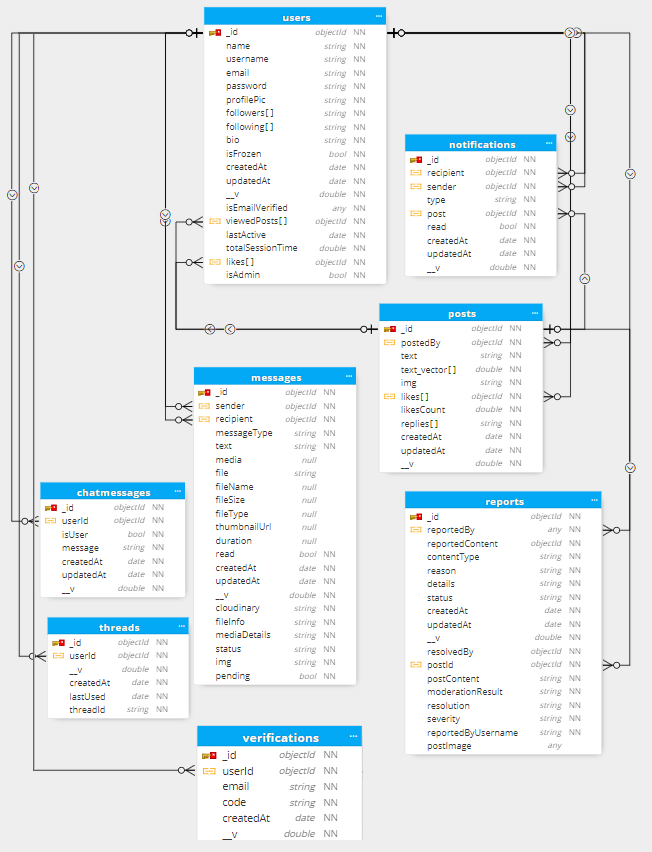
\includegraphics[width=1\textwidth]{image/MoHinh/13.png}
%     \caption{Hình ảnh Quan hệ giữa các bảng}
%     \label{fig:quan_he_giua_cac_banng}
% \end{figure}

\newpage
\section{\textbf{Mô hình,thực nghiệm và đánh giá}}

% \textbf{1. Hệ thống kiểm duyệt nội dung đa phương thức}


% \begin{figure}[H]
%     \centering
%     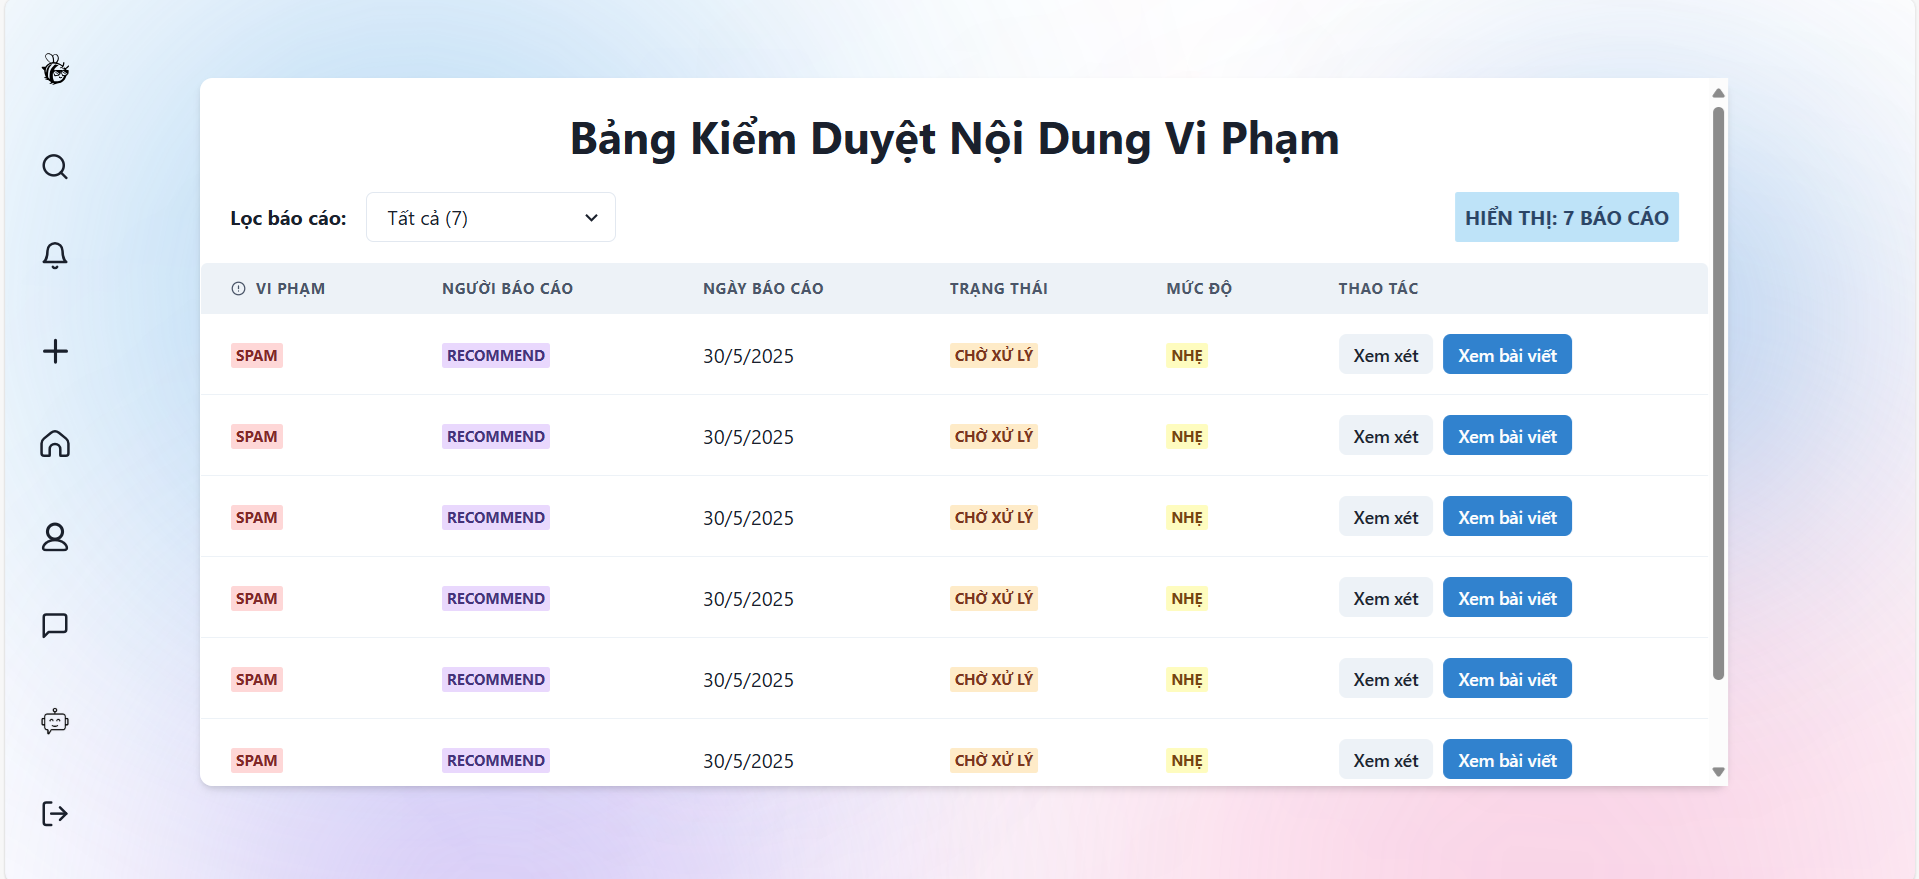
\includegraphics[width=1\textwidth]{image/thucnghiem/report.png}
%     \caption{Hình ảnh Bảng kiểm duyệt nội dung vi phạm}
%     \label{fig:bao_cao}
% \end{figure}



% \textbf{Phân tích thông minh với OpenAI Moderation API}
% \begin{itemize}
%     \item \textbf{Kiểm duyệt đa phương thức}: Phân tích cả văn bản và hình ảnh trong moderationService.ts
%     \item \textbf{Phân loại mức độ nghiêm trọng}: Tự động xác định low, medium, high dựa trên điểm số vi phạm
%     \item \textbf{Xử lý thời gian thực}: Kiểm tra ngay khi đăng bài, tạo báo cáo tự động trong moderationController.ts
% \end{itemize}

% \textbf{Dashboard quản trị viên}
% \begin{itemize}
%     \item Giao diện quản lý báo cáo vi phạm hoàn chỉnh trong AdminPage.tsx
%     \item Workflow phê duyệt/từ chối với lý do chi tiết
%     \item Thống kê vi phạm theo thời gian và mức độ
% \end{itemize}

% \newpage

% \textbf{2. Tìm kiếm ngữ nghĩa vector-based}

% \begin{figure}[H]
%     \centering
%     
\includegraphics[width=1\textwidth]{image/thucnghiem/ngunghia.png}
%     \caption{Hình ảnh Ngữ nghĩa}
%     \label{fig:nghu_nghia}
% \end{figure}

% \begin{itemize}
%     \item \textbf{Vector embeddings}: Sử dụng OpenAI text-embedding-3-large trong embeddingService.ts
%     \item \textbf{Elasticsearch kNN}: Tìm kiếm vector với độ chính xác cao
%     \item \textbf{Tìm kiếm đa trường}: Kết hợp users, posts, comments trong một truy vấn
% \end{itemize}

% \textbf{Indexing thông minh}
% \begin{itemize}
%     \item \textbf{Auto-indexing}: Tự động tạo embeddings khi tạo bài viết mới
%     \item \textbf{Batch processing}: Script đánh index hàng loạt trong indexAdvancedData.ts
% \end{itemize}
% \newpage
% \textbf{3. Hệ thống nhắn tin thời gian thực}
% \begin{figure}[H]
%     \centering
%     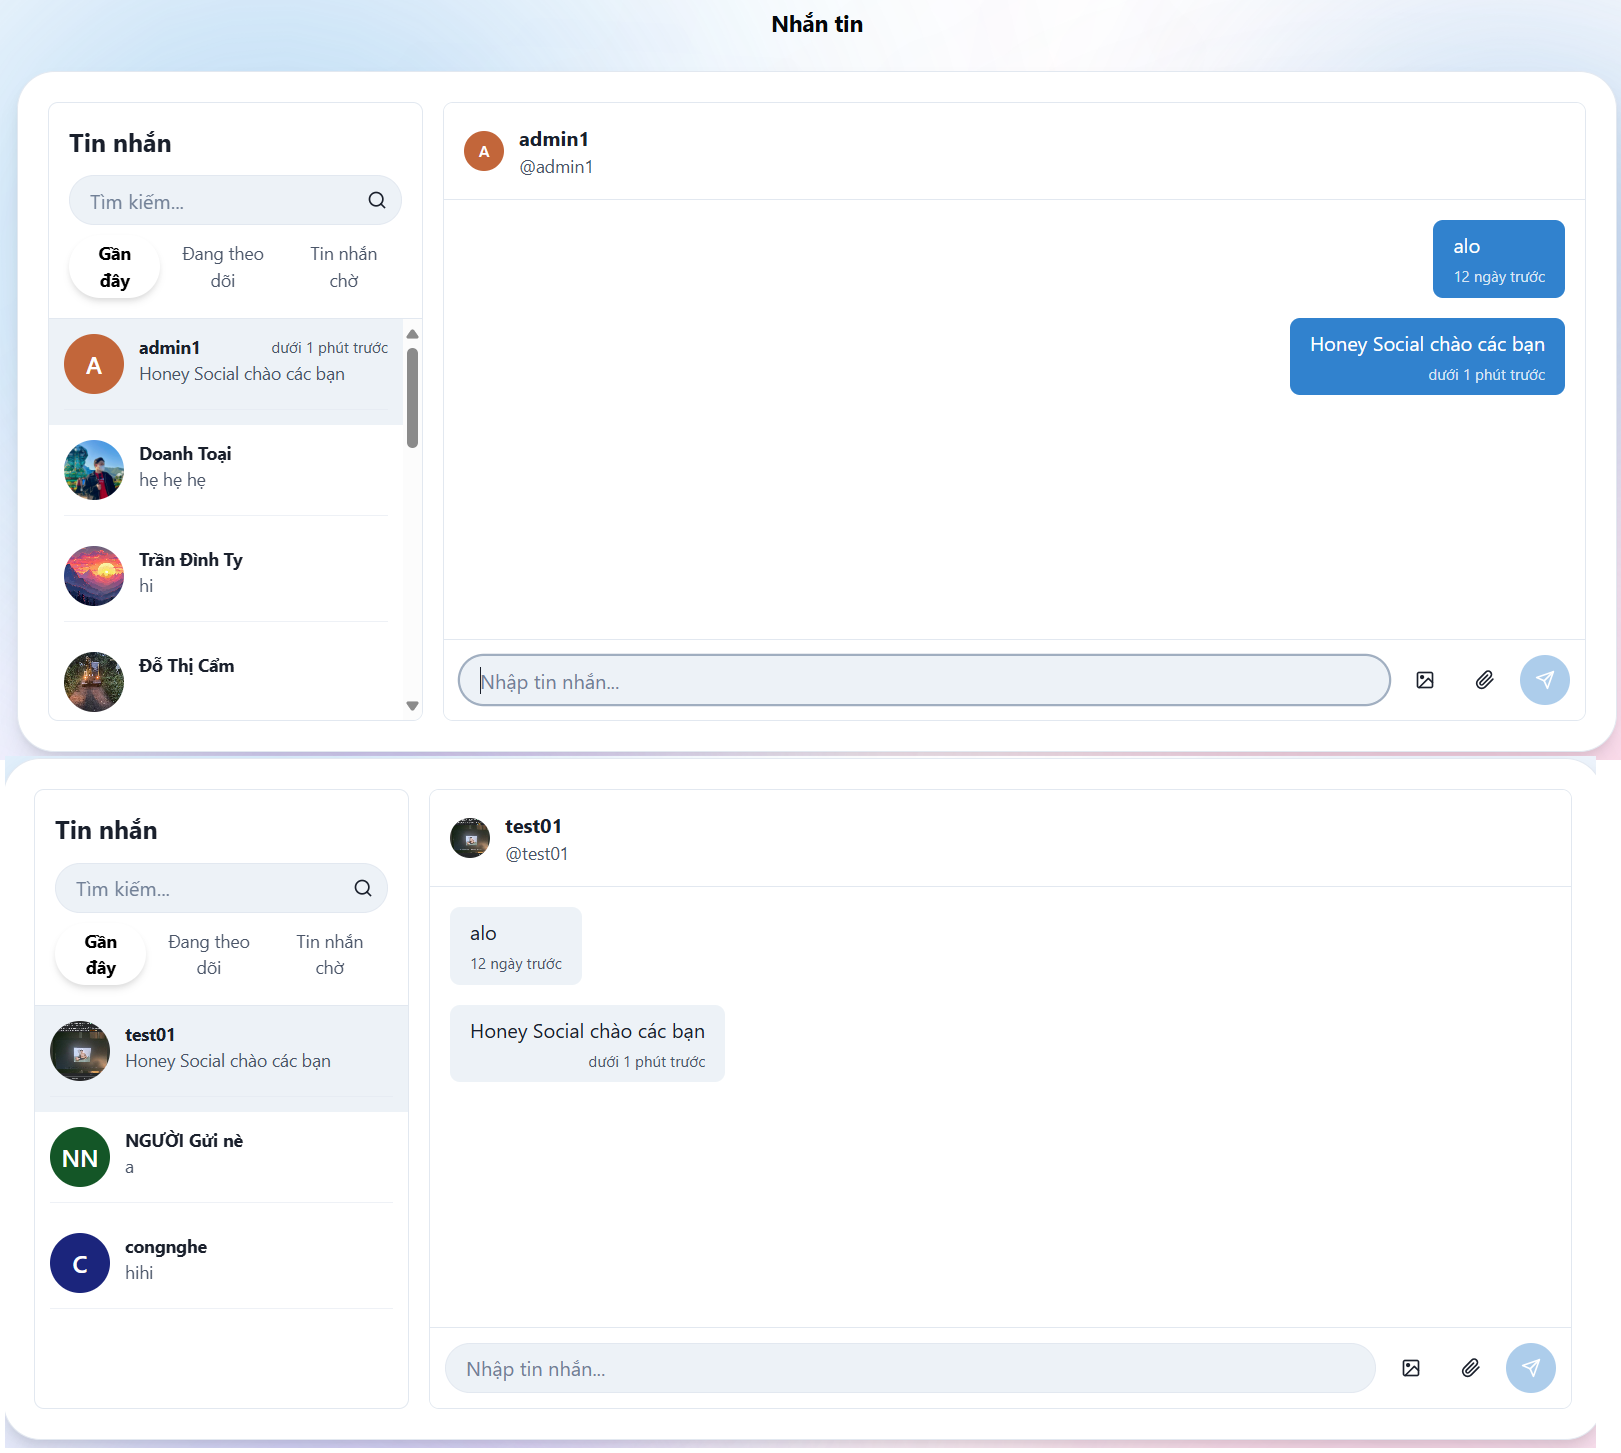
\includegraphics[width=1\textwidth]{image/thucnghiem/hinhve.png}
%     \caption{Hình ảnh Nhắn tin}
%     \label{fig:nhan_tin}
% \end{figure}
% \textbf{Tính năng nâng cao}
% \begin{itemize}
%     \item \textbf{Socket.io real-time}: Tin nhắn tức thời với read receipts trong socket.ts
%     \item \textbf{Message pending system}: Bảo vệ quyền riêng tư với workflow chấp nhận tin nhắn
%     \item \textbf{Media sharing}: Upload ảnh/file với Cloudinary integration
% \end{itemize}

% \textbf{Quản lý cuộc trò chuyện}
% \begin{itemize}
%     \item \textbf{Conversation management}: Giao diện chat với tabs Recent, Following, Pending
%     \item \textbf{Auto-follow on accept}: Tự động follow khi chấp nhận tin nhắn
%     \item \textbf{File upload}: Hỗ trợ nhiều định dạng với preview
% \end{itemize}

% \textbf{4. Hệ thống gợi ý thông minh}
% \begin{figure}[H]
%     \centering
%     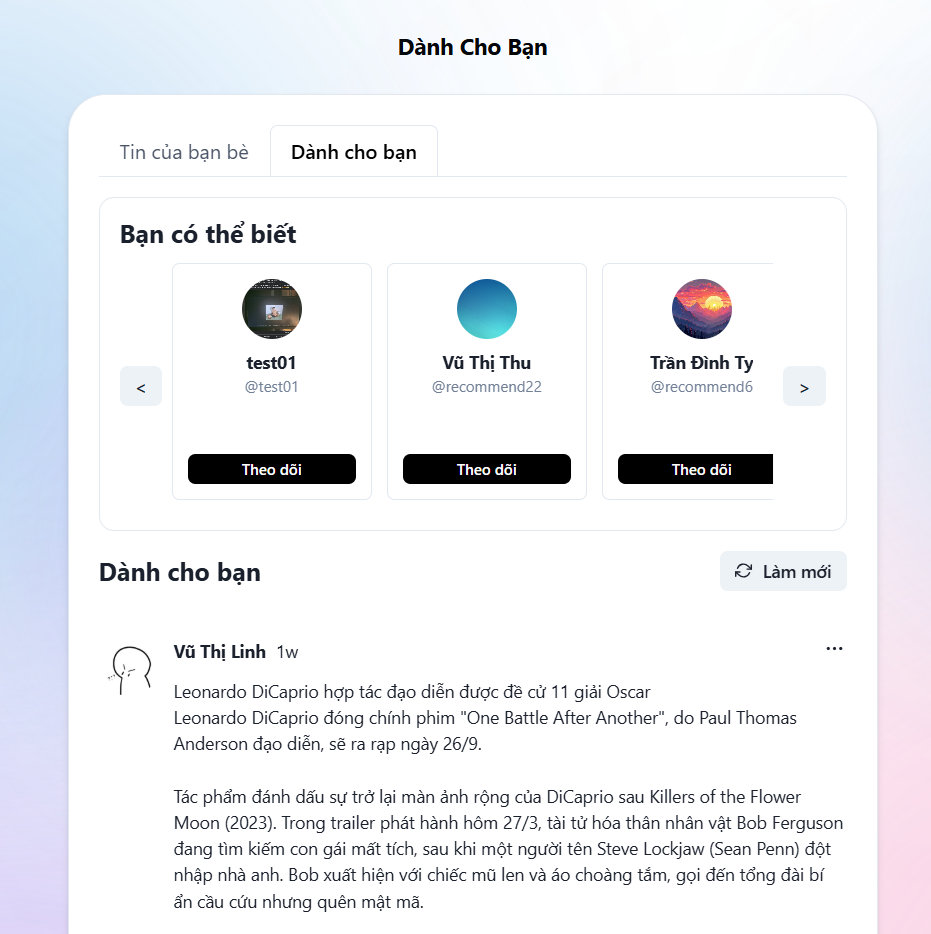
\includegraphics[width=1\textwidth]{image/thucnghiem/recommend.png}
%     \caption{Hình ảnh Gợi ý}
%     \label{fig:goi_y}
% \end{figure}
% \textbf{Gợi ý kết bạn dựa trên social graph}
% \begin{itemize}
%     \item \textbf{Mutual connections}: Phân tích kết nối chung trong recommendationController.ts
%     \item \textbf{Popularity scoring}: Tính điểm uy tín dựa trên followers/following ratio
%     \item \textbf{Elasticsearch aggregation}: Query phức tạp để tìm gợi ý tối ưu
% \end{itemize}

% \textbf{Gợi ý nội dung cá nhân hóa}
% \begin{itemize}
%     \item \textbf{Vector similarity}: So sánh embedding của bài viết đã thích
%     \item \textbf{Weighted combination}: Kết hợp nhiều vector với trọng số
%     \item \textbf{Fallback mechanism}: Đảm bảo luôn có gợi ý dù thiếu dữ liệu
% \end{itemize}

% \textbf{5. Trợ lý AI tích hợp}
% \begin{figure}[H]
%     \centering
%     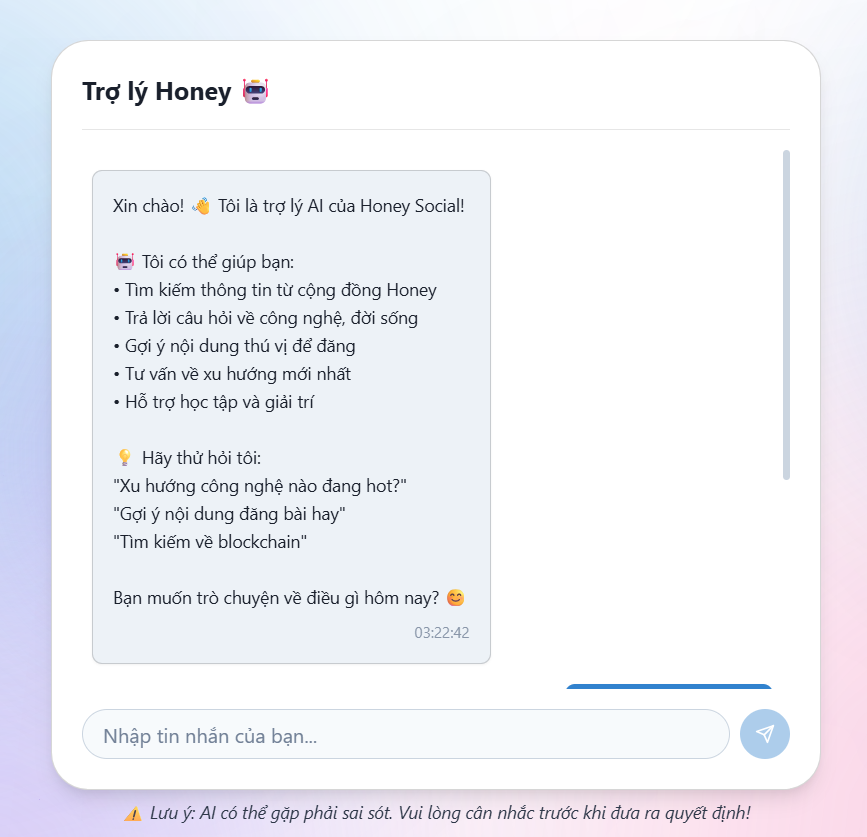
\includegraphics[width=1\textwidth]{image/thucnghiem/ai.png}
%     \caption{Hình ảnh Trí tuệ nhân tạo}
%     \label{fig:tri_tue_nhan_tao}
% \end{figure}
% \textbf{OpenAI Assistant với context}
% \begin{itemize}
%     \item \textbf{Thread-based conversation}: Lưu trữ lịch sử trò chuyện trong openaiService.ts
%     \item \textbf{Context awareness}: AI hiểu thông tin user như bio, posts, likes
%     \item \textbf{File search integration}: Tìm kiếm thông tin từ database
% \end{itemize}

% \textbf{Giao diện chat thông minh}
% \begin{itemize}
%     \item \textbf{Quick suggestions}: Gợi ý câu hỏi nhanh trong ChatAI.tsx
%     \item \textbf{Real-time typing}: Hiệu ứng typing indicator
%     \item \textbf{Message history}: Lưu trữ và khôi phục cuộc trò chuyện
% \end{itemize}

% \textbf{6. Hệ thống xác minh email}
% \begin{figure}[H]
%     \centering
%     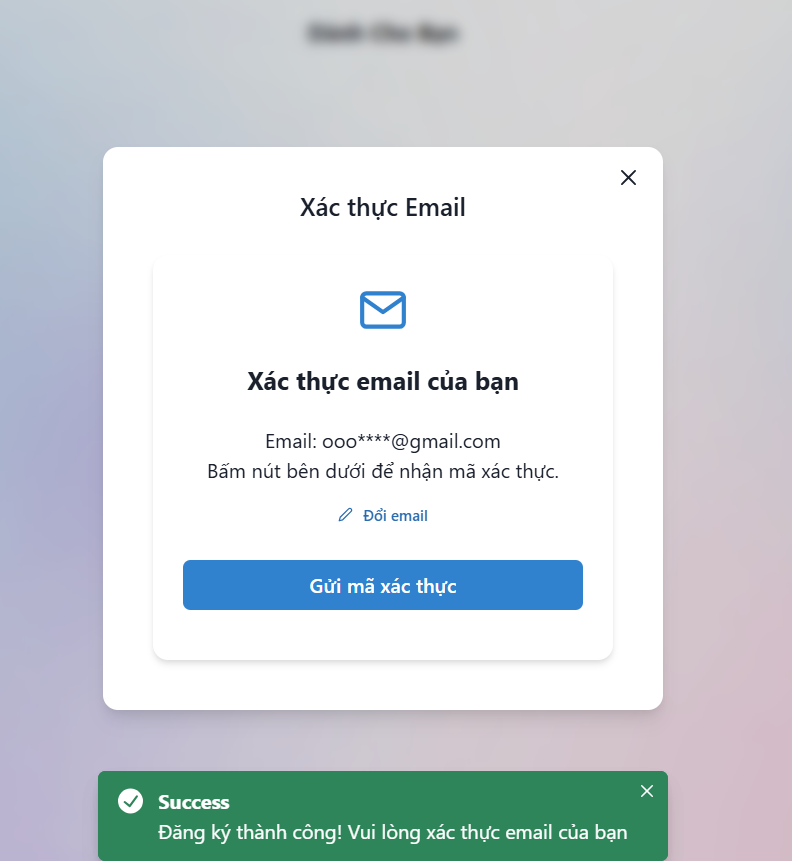
\includegraphics[width=1\textwidth]{image/thucnghiem/mail.png}
%     \caption{Hình ảnh Xác nhận mail}
%     \label{fig:xac_nhan}
% \end{figure}
% \textbf{Security với UX tối ưu}
% \begin{itemize}
%     \item \textbf{Rate limiting}: Chống spam với cooldown 45 giây trong verificationController.ts
%     \item \textbf{Email masking}: Bảo mật thông tin email
%     \item \textbf{Protected routes}: Component bảo vệ yêu cầu xác minh trong EmailProtectedRoute.tsx
% \end{itemize}

% \textbf{Workflow hoàn chỉnh}
% \begin{itemize}
%     \item \textbf{Email change flow}: Quy trình đổi email an toàn
%     \item \textbf{Queue processing}: Xử lý email bất đồng bộ
%     \item \textbf{Modal integration}: Giao diện xác minh liền mạch
% \end{itemize}

% \textbf{Background processing}
% \begin{itemize}
%     \item \textbf{Social actions worker}: Xử lý like/follow bất đồng bộ trong socialActionsWorker.ts
%     \item \textbf{Queue-based architecture}: Tách biệt logic nặng khỏi response time
%     \item \textbf{Error handling}: Retry mechanism và fallback
% \end{itemize}
% \newpage
% \textbf{7. Bảo mật và triển khai}
% \begin{figure}[H]
%     \centering
%     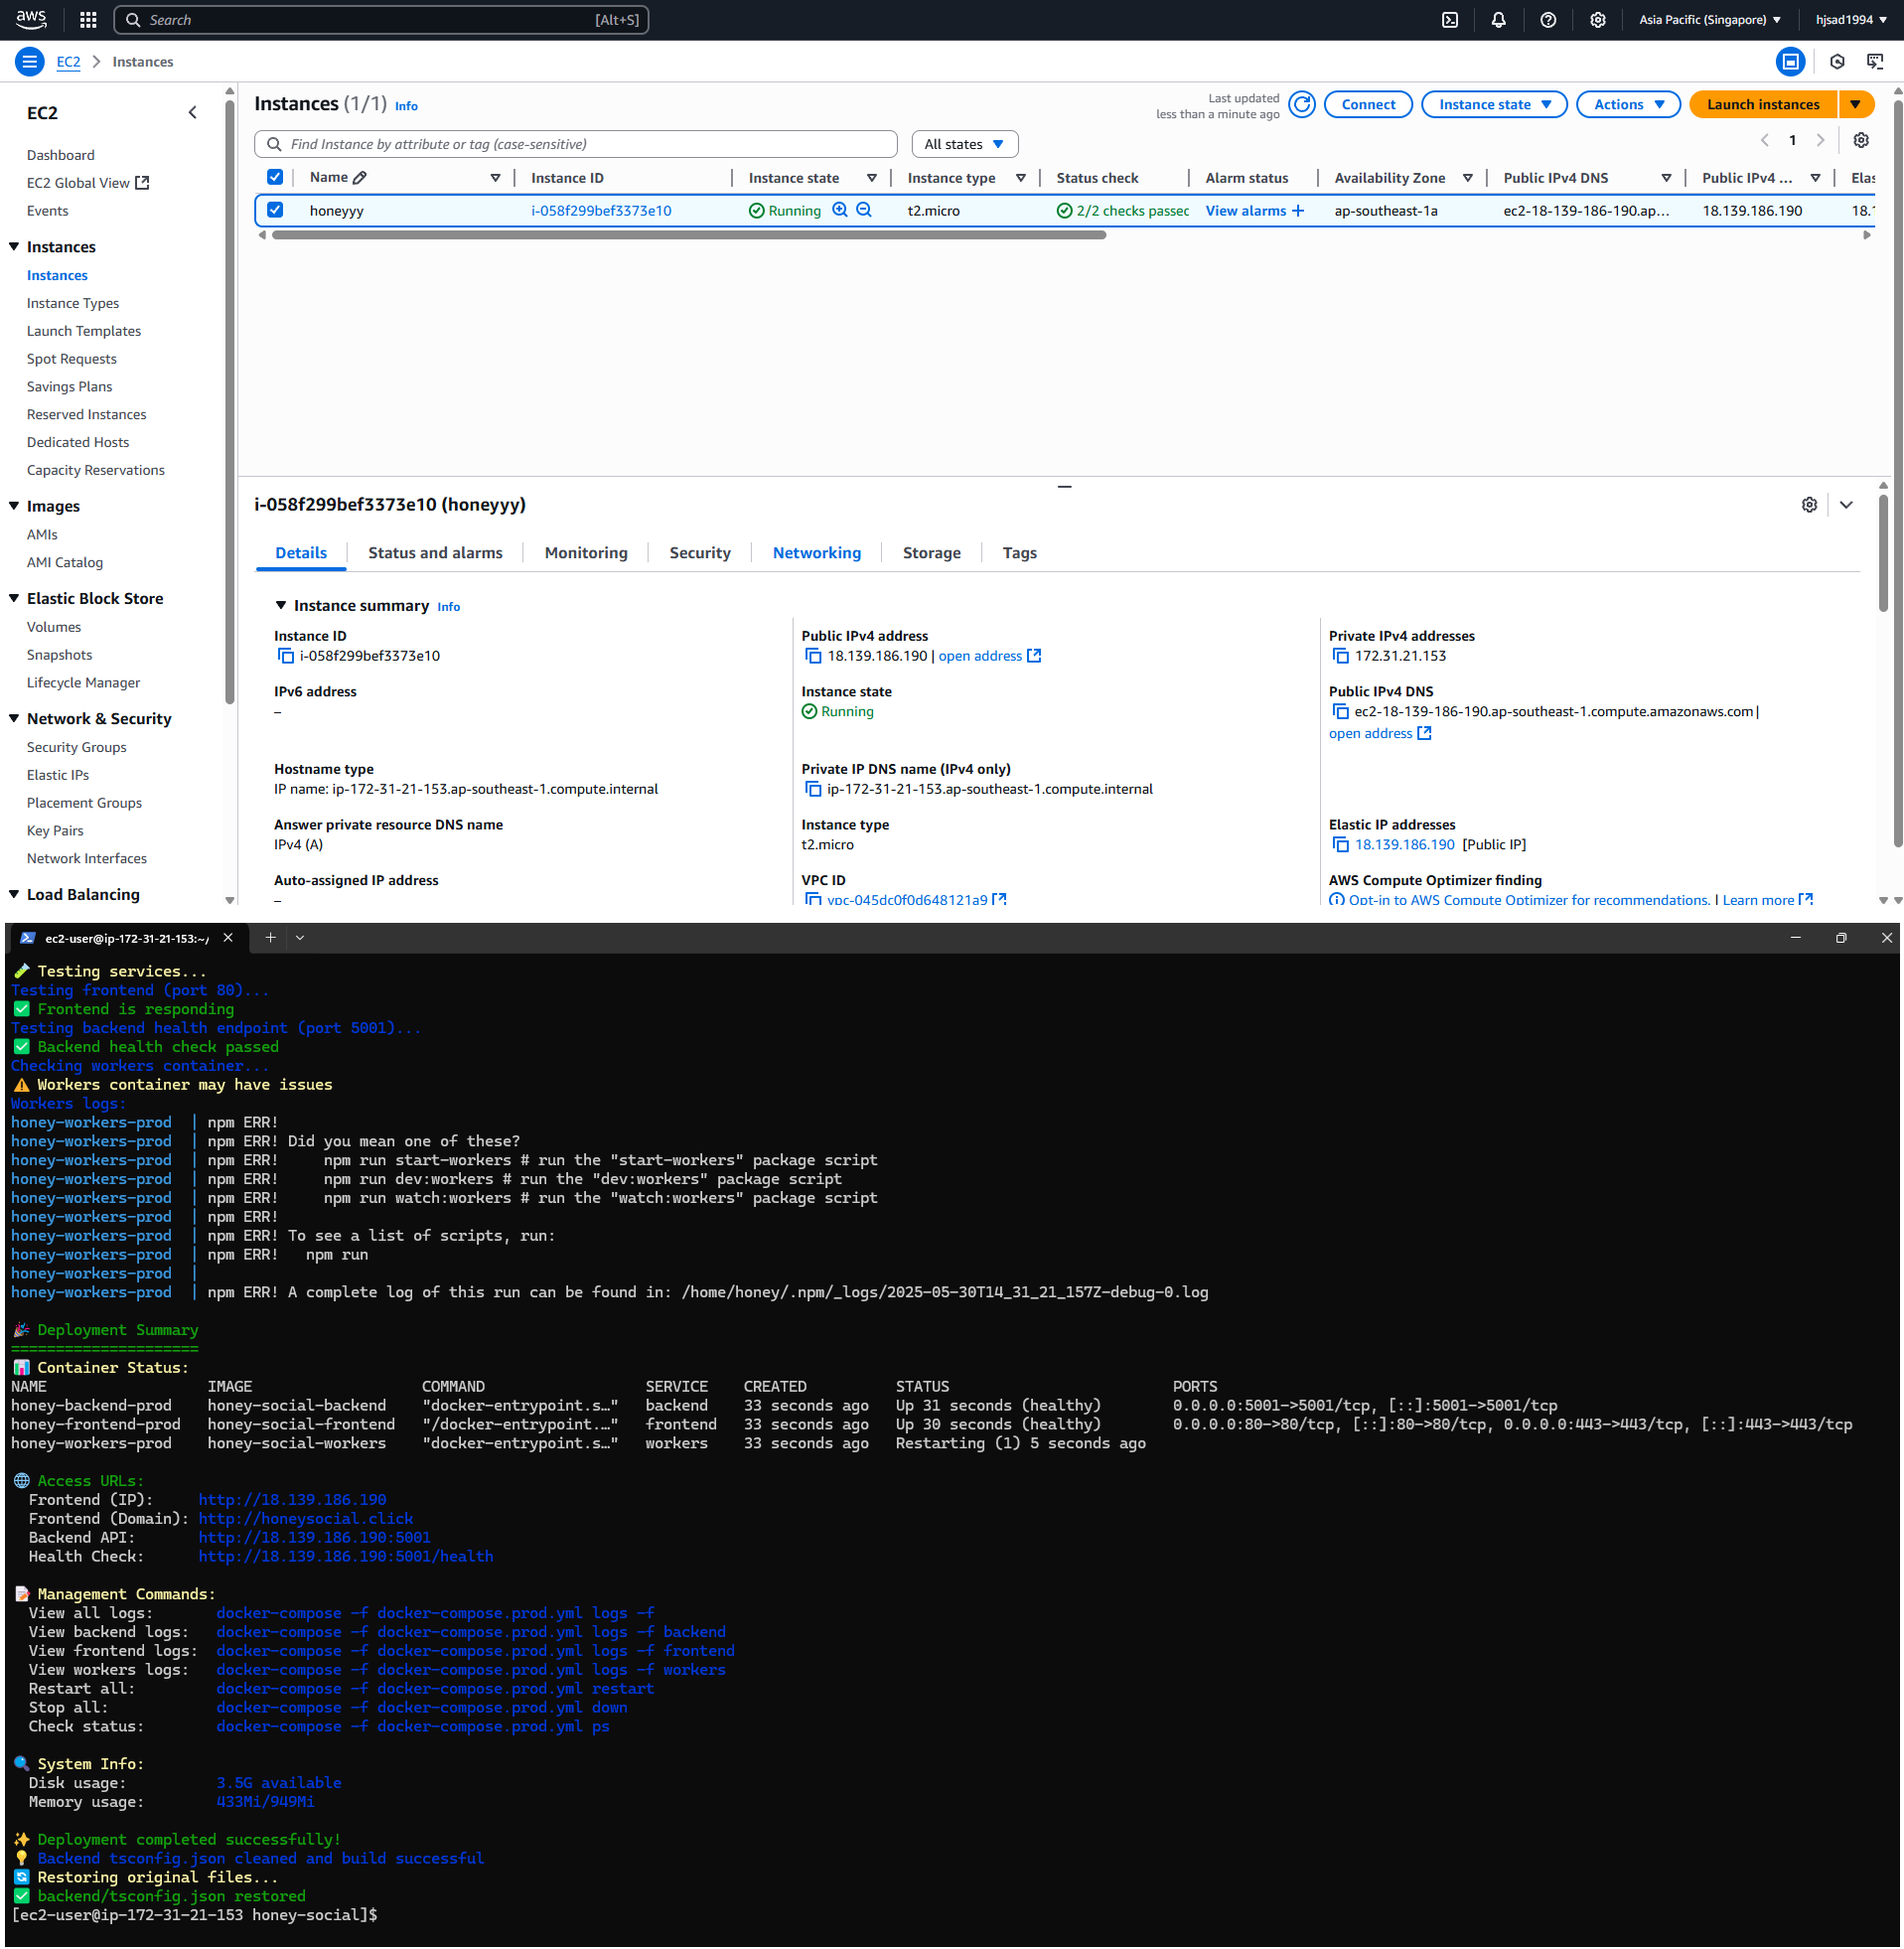
\includegraphics[width=1\textwidth]{image/thucnghiem/Deployment.png}
%     \caption{Hình ảnh Deployment}
%     \label{fig:deployment}
% \end{figure}

% \textbf{SSL Certificate tự động}
% \begin{itemize}
%     \item \textbf{Let's Encrypt SSL}: Certificate miễn phí cho domain honeysocial.click
%     \item \textbf{Auto-renewal}: Script tự động gia hạn certificate
%     \item \textbf{HTTPS redirect}: Tự động chuyển hướng từ HTTP sang HTTPS
% \end{itemize}

% \textbf{Deployment hoàn chỉnh}
% \begin{itemize}
%     \item \textbf{Docker containerization}: Triển khai với docker-compose
%     \item \textbf{Nginx reverse proxy}: Load balancing và SSL termination
%     \item \textbf{Production monitoring}: Health checks và logging
% \end{itemize}


% \newpage
% \section{\textbf{CHƯƠNG 6: KẾT LUẬN VÀ KIẾN NGHỊ}}


% \subsection{Kết Luận}

% \subsubsection{Tổng kết quá trình thực hiện đồ án}
% Đồ án đã thực hiện xây dựng thành công mạng xã hội Honey Social với kiến trúc hiện đại, tách biệt Frontend và Backend rõ ràng. Quá trình phát triển tuân theo phương pháp Agile, cho phép linh hoạt điều chỉnh khi gặp thách thức. Việc áp dụng các mô hình thiết kế như MVC, đã giúp mã nguồn có cấu trúc tốt, dễ bảo trì và mở rộng.

% \subsubsection{Kết quả đạt được}
% \begin{enumerate}
%     \item \textbf{Hệ thống đa chức năng} - Mạng xã hội hoàn chỉnh với các tính năng chính:
%     \begin{itemize}
%         \item Đăng bài viết với hình ảnh và văn bản
%         \item Hệ thống chat realtime giữa người dùng
%         \item Trợ lý AI thông minh tích hợp
%         \item Hệ thống gợi ý nội dung dựa trên vector search
%         \item Hệ thống thông báo realtime
%         \item Tìm kiếm nâng cao với Elasticsearch
%     \end{itemize}
    
%     \item \textbf{Kiến trúc kỹ thuật hiện đại}:
%     \begin{itemize}
%         \item Frontend: React.js với state management thông qua Redux
%         \item Backend: Node.js, Express.js với TypeScript
%         \item Cơ sở dữ liệu: MongoDB kết hợp với Redis cache
%         \item WebSocket cho giao tiếp realtime
%         \item RabbitMQ cho hàng đợi xử lý bất đồng bộ
%         \item Docker cho việc phát triển và triển khai
%     \end{itemize}
    
%     \item \textbf{Hiệu năng cao}:
%     \begin{itemize}
%         \item Hệ thống cache đa tầng giúp giảm tải database
%         \item Xử lý bất đồng bộ các tác vụ nặng như phân tích nội dung, moderation
%         \item Vector search cho khả năng tìm kiếm và gợi ý thông minh
%     \end{itemize}
% \end{enumerate}

% \subsubsection{Hạn chế và thách thức}
% \begin{enumerate}
%     \item \textbf{Độ phức tạp của hệ thống}:
%     \begin{itemize}
%         \item Cache invalidation khó xử lý đúng trong mọi tình huống
%         \item Phân tán microservice làm tăng độ phức tạp vận hành
%     \end{itemize}
    
%     \item \textbf{Hiệu năng của AI}:
%     \begin{itemize}
%         \item Thời gian phản hồi của ChatAI đôi khi còn chậm
%         \item Vector embedding tốn kém tài nguyên khi hệ thống lớn
%     \end{itemize}
    
%     \item \textbf{Giới hạn tích hợp}:
%     \begin{itemize}
%         \item Chưa có ứng dụng di động native
%         \item Hệ thống gợi ý cần thêm dữ liệu để tăng độ chính xác
%     \end{itemize}
% \end{enumerate}

% \subsection{Kiến nghị và hướng phát triển}

% \subsubsection{Phát triển ứng dụng di động}
% Xây dựng ứng dụng di động native cho iOS và Android sử dụng React Native hoặc Flutter để tận dụng codebase hiện có, đồng thời cải thiện trải nghiệm người dùng trên thiết bị di động với các tính năng như thông báo đẩy, camera tích hợp và trải nghiệm offline.

% \subsubsection{Nâng cấp hệ thống gợi ý nội dung}
% Cải tiến hệ thống gợi ý bằng cách kết hợp các yếu tố hành vi người dùng (thời gian xem, tương tác), ngữ cảnh (thời gian, vị trí) và mạng xã hội (kết nối giữa người dùng) để tạo ra gợi ý cá nhân hóa chính xác hơn.

% \subsubsection{Triển khai AI Chatbot học tự động}
% Phát triển khả năng học tự động cho ChatAI để liên tục cải thiện chất lượng phản hồi dựa trên tương tác của người dùng. Triển khai fine-tuning mô hình để chatbot hiểu tốt hơn ngữ cảnh và văn hóa cụ thể của cộng đồng Honey Social.

% \subsubsection{Tối ưu cơ chế làm mới Redis Cache}
% Cải tiến cơ chế cache với chiến lược write-through và read-through thông minh hơn, đồng thời sử dụng Redis Streams để quản lý việc làm mới cache phân tán, giảm thiểu lỗi cache inconsistency trong hệ thống nhiều node.

% \subsubsection{Cải tiến hệ thống Post Recommendation}
% Nâng cấp hệ thống gợi ý bài đăng bằng cách sử dụng kỹ thuật collaborative filtering kết hợp với vector search, đồng thời tối ưu hóa thuật toán lọc bọt (filter bubble) để đảm bảo người dùng tiếp cận được nhiều nội dung đa dạng.

% \subsubsection{Phát triển ChatboxAI nội bộ}
% Xây dựng công cụ chatbot nội bộ được huấn luyện trên dữ liệu hệ thống để hỗ trợ người quản trị trong việc phân tích xu hướng, phát hiện nội dung vi phạm, và tổng hợp báo cáo hoạt động của cộng đồng.
\clearpage
\section{TÀI LIỆU THAM KHẢO}
\begin{thebibliography}{00}

\bibitem{aws-doc}
Amazon Web Services, "Deploy a React-based single-page application to Amazon S3 and CloudFront." [Online].\\
Available: \url{https://short.com.vn/P0gh}

\bibitem{openai-moderation}
OpenAI, "Moderation Guide." [Online].\\
Available: \url{https://platform.openai.com/docs/guides/moderation}

\bibitem{openai-assistants}
OpenAI, "Assistants API Overview." [Online].\\
Available: \url{https://platform.openai.com/docs/assistants/overview}

\bibitem{openai-embeddings}
OpenAI, "Embeddings Guide." [Online].\\
Available: \url{https://platform.openai.com/docs/guides/embeddings}

\bibitem{cache-aside}
GeeksforGeeks, "Cache-Aside Pattern." [Online].\\
Available: \url{https://www.geeksforgeeks.org/cache-aside-pattern/}

\bibitem{elasticsearch-knowi}
Knowi, "What is Elasticsearch?" [Online].\\
Available: \url{https://www.knowi.com/blog/what-is-elastic-search/}

\bibitem{kim-2014-convolutional}
Y. Kim, "Convolutional Neural Networks for Sentence Classification," in \textit{Proceedings of the 2014 Conference on Empirical Methods in Natural Language Processing (EMNLP)}, Doha, Qatar, 2014, pp. 1746--1751.

\bibitem{10.1162/neco.1997.9.8.1735}
S. Hochreiter and J. Schmidhuber, "Long Short-Term Memory," \textit{Neural Computation}, vol. 9, no. 8, pp. 1735--1780, 1997.

\bibitem{vaswani2017attention}
A. Vaswani \textit{et al.}, "Attention Is All You Need," in \textit{Advances in Neural Information Processing Systems}, vol. 30, 2017.

\bibitem{phobert}
D. Q. Nguyen and A. T. Nguyen, "PhoBERT: Pre-trained language models for Vietnamese," in \textit{Proceedings of the 2020 Conference on Empirical Methods in Natural Language Processing: Findings}, Online, 2020, pp. 1037--1042.

\end{thebibliography}

\end{document}